\chapter[ESPACIOS VECTORIALES CON PRODUCTO INTERNO]{ESPACIOS VECTORIALES \\ CON PRODUCTO \\ INTERNO}
%\startcontents
\printchaptertableofcontents

Los espacios vectoriales con producto interno son estructuras matemáticas fundamentales que combinan dos conceptos esenciales: el espacio vectorial y el producto interno. En términos simples, un espacio vectorial con producto interno es un espacio vectorial equipado con una operación adicional llamada producto interno, que asigna a cada par de vectores un escalar en el campo subyacente.

Para comprender mejor estos espacios, es crucial entender cada componente por separado. Primero, un espacio vectorial es un conjunto de elementos, llamados vectores, sobre un campo escalar, generalmente los números reales o complejos. Este conjunto cumple ciertas propiedades, como la cerradura bajo la adición y la multiplicación por escalares, la existencia de un elemento neutro aditivo y la existencia de inversos aditivos para cada elemento (vea el \hyperref[chap:ev]{capítulo 1}).

El producto interno, por otro lado, es una operación que toma dos vectores y produce un escalar. Este producto interno debe cumplir varias propiedades, como la linealidad en su primer argumento, la simetría y la positividad definida. En términos más simples, el producto interno mide la “similitud” entre dos vectores y puede interpretarse geométricamente en espacios euclídeos como el ángulo entre ellos.

Al combinar estos dos conceptos, un espacio vectorial con producto interno es un espacio vectorial equipado con una función que asigna a cada par de vectores un escalar, de manera que esta función satisfaga las propiedades del producto interno.

Algunos ejemplos comunes de espacios vectoriales con producto interno incluyen espacios euclídeos, donde los vectores se representan como $n$-tuplas de números reales y el producto interno se define como el producto punto convencional. También, espacios de funciones, donde los vectores son funciones y el producto interno puede ser definido utilizando la integral de su producto puntual, y espacios de matrices, donde los vectores son matrices y el producto interno puede ser definido de diversas maneras, como el producto de Frobenius.

Los espacios vectoriales con producto interno tienen una amplia variedad de aplicaciones en matemáticas y física, desde el análisis funcional hasta la mecánica cuántica. Proporcionan un marco poderoso para entender la geometría y las propiedades de los vectores en contextos abstractos y concretos. Además, son fundamentales en el estudio de transformaciones lineales y la resolución de sistemas de ecuaciones lineales mediante métodos como la descomposición en valores singulares y la diagonalización de matrices hermíticas.

\section{Producto punto y proyecciones}\label{sec:orto}

En el capítulo \ref{chap:matrices}, se introdujo el concepto de multiplicación de matrices, incluyendo el producto punto (vea la definición \ref{definicion:JUNSJSNSN}) y la norma en $\RR[2]$. En este nuevo capítulo sobre espacios vectoriales con producto interno, se ampliará esta noción al considerar la norma en \( \RR[n] \) y generalizar la definición de la norma en este contexto más amplio. La comprensión previa del producto punto en la página \pageref{definicion:JUNSJSNSN} será esencial para asimilar la definición extendida de la norma en \( \RR[n] \) y explorar las propiedades asociadas en un contexto más generalizado.

\begin{observation}\label{Obs:innerproduct}
    Dados $\mathbb{u}$, $\mathbb{v} \in \RR[n]$. Es relevante destacar que el producto punto entre dos vectores $\mathbb{u}$ y $\mathbb{v}$ puede definirse de manera elegante como el producto de $\mathbb{u}^t$ y $\mathbb{v}$, es decir,
    $$\mathbb{u} \bullet \mathbb{v} = \mathbb{u}^t \mathbb{v}$$
    Pues,
    $$\mathbb{u}^t \mathbb{v} = (u_1, u_2, \dots, u_n) \begin{pmatrix} v_1 \\ v_2 \\ \vdots \\ v_n \end{pmatrix} = \sum_{i=1}^n u_i v_i$$
    Es importante señalar que con esta observación, el producto punto entre los vectores \( \mathbb{u} \) y \( \mathbb{v} \) ya no se denota con el símbolo “$\bullet$”, sino que se representa mediante la yuxtaposición entre \( \mathbb{u}^t \) y \( \mathbb{v} \). Esta observación refleja una diferencia clave en la notación utilizada para describir el producto punto en el contexto de matrices y espacios vectoriales, brindando coherencia y claridad en la exposición de conceptos algebraicos y geométricos.
\end{observation}

\begin{definition}
    Sea $\mathbb{u} \in \RR[n]$ con $\mathbb{u} = \begin{pmatrix} u_1 \\ u_2 \\ \vdots \\ u_n \end{pmatrix}$. Se define la norma del vector $\mathbb{u}$ como
    $$\| \mathbb{u} \| = \sqrt{\mathbb{u} \bullet \mathbb{u}} = \sqrt{u_1^2 + u_2^2 + \cdots + u_n^2}$$
\end{definition}

\newpage

\begin{proposition}\label{prop:norma}
    La norma satisface las siguientes propiedades: Para todo $\mathbb{u} \in \RR[n]$ y $\alpha \in \RR$
    \begin{enumerate}[label=\roman*)]
        \item $\| \mathbb{u} \| \geq 0$.
        \item $\| \mathbb{u} \| = 0$ si y solo si $\mathbb{u} = \mathbb{0}$.
        \item $\| \alpha \mathbb{u} \| = |\alpha| \| \mathbb{u} \|$.
    \end{enumerate}
    \demostracion Dado que las propiedades  (i) y (ii) son demostraciones directas, nos enfocaremos en demostrar la propiedad (iii). Sea $\mathbb{u} \in \RR[n]$ y $\alpha \in \RR$,
    \begin{align*}
        \| \alpha \mathbb{u} \|^2 & = (\alpha \mathbb{u}) \bullet (\alpha \mathbb{u}) \\
        & = \alpha \big( \mathbb{u} \bullet (\alpha \mathbb{u}) \big) \\
        & = \alpha \cdot \alpha (\mathbb{u} \bullet \mathbb{u}) \\
        & = \alpha^2 \| \mathbb{u} \|^2
    \end{align*}
    Así,
    $$\| \alpha \mathbb{u} \|^2 = \alpha^2 \| \mathbb{u} \|^2$$
    Por el curso de Cálculo I, sabemos que $\sqrt{\alpha^2} = |\alpha|$. Así pues, se hereda que
    $$\big| \| \alpha \mathbb{u} \| \big| = |\alpha| \, \big| \| \mathbb{u} \| \big|$$
    Finalmente, de la propiedad (i) de esta proposición se sigue que
    $$\| \alpha \mathbb{u} \| = |\alpha| \| \mathbb{u} \|$$
\end{proposition}

\begin{observation}
    A la norma $\| \quad \|$ definida anteriormente, se le llamará norma euclidiana.
\end{observation}

\begin{definition}
    Al espacio vectorial con la norma $\| \quad \|$, se le llamará espacio euclidiano.
\end{definition}

\begin{definition}\label{def:vectoresortogonales}
    Dados $\mathbb{u}$, $\mathbb{v} \in \RR[n]$. Decimos que $\mathbb{u}$ es ortogonal a $\mathbb{v}$ o que $\mathbb{v}$ es ortogonal a $\mathbb{u}$, si $\mathbb{u} \bullet \mathbb{v} = 0$. En este caso, escribiremos $\mathbb{u} \perp \mathbb{v}$.
\end{definition}

\begin{definition}
    Dado $\mathbb{u} \in \RR[n]$. Se define al vector unitario, denotado por $\hat{\mathbb{u}}$, como
    $$\hat{\mathbb{u}} = \frac{1}{\| \mathbb{u} \|} \mathbb{u}$$
    Este vector tendrá como norma igual a $1$, es decir, $\left\| \hat{\mathbb{u}} \right\| = 1$.
\end{definition}

\begin{definition}\label{def:conjunto_ortonormal}
    Dados $\mathbb{u}_1$, $\mathbb{u}_2$, $\dots$, $\mathbb{u}_k \in \RR[n]$.
    \begin{enumerate}[label=\roman*)]
        \item Se dice que el conjunto $\left\{ \mathbb{u}_1, \mathbb{u}_2, \dots, \mathbb{u}_k \right\}$ es un conjunto ortogonal de vectores si $\mathbb{u}_i \bullet \mathbb{u}_j = 0$, $\forall i \neq j$,
        \item Si además, se cumple que $\| \mathbb{u}_i \| = 1$ para $i = 1$, $2$, $\dots$, $k$, entonces diremos que el conjunto $\left\{ \mathbb{u}_1, \mathbb{u}_2, \dots, \mathbb{u}_k \right\}$ es un conjunto ortonormal de vectores.
    \end{enumerate}
\end{definition}

\begin{example}
    En $\RR[3]$, observemos que el conjunto $\left\{ \begin{pmatrix} 1 \\ 0 \\ 0 \end{pmatrix}, \begin{pmatrix} 0 \\ 1 \\ 0 \end{pmatrix}, \begin{pmatrix} 0 \\ 0 \\ 1 \end{pmatrix} \right\}$ es un conjunto ortonormal. Para probarlo, primero verifiquemos que es un conjunto ortogonal como sigue:
    $$\begin{pmatrix} 1 \\ 0 \\ 0 \end{pmatrix} \bullet \begin{pmatrix} 0 \\ 1 \\ 0 \end{pmatrix} = 0 \qquad \begin{pmatrix} 1 \\ 0 \\ 0 \end{pmatrix} \bullet \begin{pmatrix} 0 \\ 0 \\ 1 \end{pmatrix} = 0 \qquad \begin{pmatrix} 0 \\ 1 \\ 0 \end{pmatrix} \bullet \begin{pmatrix} 0 \\ 0 \\ 1 \end{pmatrix} = 0$$\newpage\noindent
    Por lo tanto, el conjunto es ortogonal. Luego, calculamos las normas:
    $$\left\| \begin{pmatrix} 1 \\ 0 \\ 0 \end{pmatrix} \right\| = 1 \qquad \left\| \begin{pmatrix} 0 \\ 1 \\ 0 \end{pmatrix} \right\| = 1 \qquad \left\| \begin{pmatrix} 0 \\ 0 \\ 1 \end{pmatrix} \right\| = 1$$
    Por tanto, el conjunto $\left\{ \begin{pmatrix} 1 \\ 0 \\ 0 \end{pmatrix}, \begin{pmatrix} 0 \\ 1 \\ 0 \end{pmatrix}, \begin{pmatrix} 0 \\ 0 \\ 1 \end{pmatrix} \right\}$ es un conjunto ortonormal.
\end{example}

\begin{theorem}\label{ortoindependiente}
    Sean $\mathbb{u}_1$, $\mathbb{u}_2$, $\dots$, $\mathbb{u}_k \in \RR[n]$. Si $\left\{ \mathbb{u}_1, \mathbb{u}_2, \dots, \mathbb{u}_k \right\}$ es un conjunto ortogonal de vectores diferentes del vector cero, entonces dicho conjunto es linealmente independiente. \\
    \demostracion Ya que $\left\{ \mathbb{u}_1, \mathbb{u}_2, \dots, \mathbb{u}_k \right\}$ es un conjunto ortogonal, entonces $\mathbb{u}_i \bullet \mathbb{u}_j = 0$, $\forall i \neq j$ con $i, j = 1, 2, \dots, k$. Sea
    $$\mathbb{0} = \alpha_1\mathbb{u}_1 + \alpha_2\mathbb{u}_2 + \cdots + \alpha_k\mathbb{u}_k$$
    con $\alpha_i \in \RR$, debemos probar que $\alpha_i = 0$ para $i = 1, 2, \dots, k$. Así,
    \begin{align*}
        0 = \mathbb{u}_i \bullet \mathbb{0} & = \mathbb{u}_i \bullet \left( \alpha_1\mathbb{u}_1 + \alpha_2\mathbb{u}_2 + \cdots + \alpha_k\mathbb{u}_k \right) \\
        & = \mathbb{u}_i \bullet ( \alpha_1\mathbb{u}_1) + \mathbb{u}_i \bullet (\alpha_2\mathbb{u}_2) + \cdots + \mathbb{u}_i \bullet (\alpha_i\mathbb{u}_i) + \cdots + \mathbb{u}_i \bullet (\alpha_k\mathbb{u}_k) \\
        & = \alpha_1 ( \mathbb{u}_i \bullet \mathbb{u}_1) + \alpha_2 (\mathbb{u}_i \bullet \mathbb{u}_2) + \cdots + \alpha_i (\mathbb{u}_i \bullet \mathbb{u}_i) + \cdots + \alpha_k (\mathbb{u}_i \bullet \mathbb{u}_k) \\
        & = \alpha_1 \cdot 0 + \alpha_2 \cdot 0 + \cdots + \alpha_i \| \mathbb{u}_i \|^2 + \cdots + \alpha_k \cdot 0
    \end{align*}
    Como $\mathbb{u}_i \neq \mathbb{0}$ por hipótesis, $\| \mathbb{u}_i \|^2 > 0$ y se tiene $\alpha_i = 0$ para $i = 1, 2, \dots, k$. Por tanto, $\mathbb{u}_1$, $\mathbb{u}_2$, $\dots$, $\mathbb{u}_k$ son linealmente independientes.
\end{theorem}

Consideremos $\mathbb{u}$ y $\mathbb{v}$ dos vectores arbitrarios pero fijos. Por el curso de Geometría Analítica, podemos graficarlos como sigue:
\begin{figure}[h!]
    \centering
    \begin{tikzpicture}[scale=1.3]
        \coordinate (O) at (0,0);
        \coordinate (X) at (-2,2);
        \coordinate (Y) at (3,2);
        \draw[-latex] (O) -- (Y) node[right] {$\mathbb{u}$};
        \draw[-latex] (O) -- (X) node[left] {$\mathbb{v}$};
        \draw (X) -- (Y);
        \pic[draw, -, "$\theta$", angle eccentricity=1.7,angle radius=0.4cm] {angle = Y--O--X};
        \node at (0.5,2) [above] {$\mathbb{v} - \mathbb{u}$};
    \end{tikzpicture}
    \caption{Gráfica de los vectores $\mathbb{u}$ y $\mathbb{v}$}
\end{figure}

De acuerdo con la ley de cosenos tenemos que
\begin{equation}
    \| \mathbb{v} - \mathbb{u} \|^2 = \| \mathbb{v} \|^2 + \| \mathbb{u} \|^2 - 2 \| \mathbb{v} \| \| \mathbb{u} \| \cos \theta \label{primeroya}
\end{equation}
Ahora
\begin{align*}
    \| \mathbb{v} - \mathbb{u} \|^2 & = (\mathbb{v} - \mathbb{u}) \bullet (\mathbb{v} - \mathbb{u}) \\
    & = (\mathbb{v} - \mathbb{u}) \bullet \mathbb{v} + (\mathbb{v} - \mathbb{u}) \bullet (-\mathbb{u}) \\
    & = \mathbb{v} \bullet (\mathbb{v} - \mathbb{u}) + (-\mathbb{u}) \bullet (\mathbb{v} - \mathbb{u}) \\
    & = \mathbb{v} \bullet \mathbb{v} + \mathbb{v} \bullet (-\mathbb{u}) + (-\mathbb{u}) \bullet \mathbb{v} + (-\mathbb{u}) \bullet (-\mathbb{u}) \\
    & = \| \mathbb{v} \|^2 + \mathbb{v} \bullet (-1 \cdot \mathbb{u}) + (-1 \cdot \mathbb{u}) \bullet \mathbb{v} + \| - \mathbb{u} \|^2 \\
    & = \| \mathbb{v} \|^2 + (-1) (\mathbb{v} \bullet \mathbb{u}) + (-1)(\mathbb{u} \bullet \mathbb{v}) + (-1)^2 \| \mathbb{u} \|^2 \\
    & = \| \mathbb{v} \|^2 - 2(\mathbb{u} \bullet \mathbb{v}) + \| \mathbb{u} \|^2
\end{align*}
Por tanto
\begin{equation}
    \| \mathbb{v} - \mathbb{u} \|^2 = \| \mathbb{v} \|^2 - 2(\mathbb{u} \bullet \mathbb{v}) + \| \mathbb{u} \|^2 \label{segundoya}
\end{equation}
De \eqref{primeroya} y \eqref{segundoya},
$$\| \mathbb{v} \|^2 + \| \mathbb{u} \|^2 - 2 \| \mathbb{v} \| \| \mathbb{u} \| \cos \theta = \| \mathbb{v} \|^2 - 2(\mathbb{u} \bullet \mathbb{v}) + \| \mathbb{u} \|^2$$\newpage\noindent
entonces
$$\| \mathbb{v} \| \| \mathbb{u} \| \cos \theta = \mathbb{v} \bullet \mathbb{u}$$
Por tanto,
\begin{equation}
    \cos \theta = \frac{\mathbb{v} \bullet \mathbb{u}}{\| \mathbb{v} \| \| \mathbb{u} \|}
\end{equation}

\begin{theorem}[Desigualdad de Cauchy-Schwarz]\label{theo:Cauchy-Schwarz}
    Dados dos vectores $\mathbb{u}$ y $\mathbb{v}$. Se cumple la desigualdad\infoBulle{
    La condición
    $$|\mathbb{u} \bullet \mathbb{v}| \leq \| \mathbb{u} \| \| \mathbb{v} \|$$
    es equivalente a
    $$(\mathbb{u} \bullet \mathbb{v})^2 \leq \| \mathbb{u} \|^2 \| \mathbb{v} \|^2$$
    }
    $$|\mathbb{u} \bullet \mathbb{v}| \leq \| \mathbb{u} \| \| \mathbb{v} \|$$
    \demostracion Del resultado anterior, tenemos que
    $$\mathbb{u} \bullet \mathbb{v} = \| \mathbb{u} \| \| \mathbb{v} \| \cos \theta$$
    entonces
    \begin{align*}
        |\mathbb{u} \bullet \mathbb{v}| & = \| \mathbb{u} \| \| \mathbb{v} \| \, |\cos \theta| \\
        & \leq \| \mathbb{u} \| \| \mathbb{v} \| \cdot 1
    \end{align*}
    Por lo tanto, $|\mathbb{u} \bullet \mathbb{v}| \leq \| \mathbb{u} \| \| \mathbb{v} \|$.
\end{theorem}

\begin{observation}
    Se cumple la igualdad
    $$|\mathbb{u} \bullet \mathbb{v}| = \| \mathbb{u} \| \| \mathbb{v} \|$$
    si $\mathbb{u} \bullet \mathbb{v} = 0$ y si $\mathbb{u}$ y $\mathbb{v}$ son linealmente dependientes. \\
    \demostracion Sean $\mathbb{u}$ y $\mathbb{v}$ linealmente dependientes, entonces
    $$\mathbb{v} = c \mathbb{u}, \text{ con } c \in \RR$$
    Así,
    \begin{align*}
        |\mathbb{u} \bullet \mathbb{v}| & = |\mathbb{u} \bullet (c \mathbb{u})| \\
        & = |c| |\mathbb{u} \bullet \mathbb{u}| \\
        & = |c| \| \mathbb{u} \| \| \mathbb{u} \|
    \end{align*}
    Además,
    \begin{align*}
        \| \mathbb{u} \| \| \mathbb{v} \| & = \| \mathbb{u} \| \| c \mathbb{u} \| \\
        & = \| \mathbb{u} \| \, |c| \, \| \mathbb{u} \| \\
        & = |c| \| \mathbb{u} \| \| \mathbb{u} \|
    \end{align*}
    De lo anterior, se sigue que
    $$|\mathbb{u} \bullet \mathbb{v}| = \| \mathbb{u} \| \| \mathbb{v} \|$$
\end{observation}

\begin{definition}
    Sea $\mathbb{u}$, $\mathbb{v} \in \RR[n]$, entonces al vector $\mathbb{w}$, como se muestra en la figura \ref{proyeccion}, se le llama proyección ortogonal del vector $\mathbb{v}$ sobre el vector $\mathbb{u}$ y se denotará por $\mathbb{w} = \proy_{\mathbb{u}} \mathbb{v}$.\sideFigure[\label{proyeccion}]{
    \begin{tikzpicture}
        \coordinate (O) at (0,0);
        \coordinate (V) at (2.5,2.5);
        \coordinate (U) at (5,0);
        \draw[latex-latex] (V) node[above] {$\mathbb{v}$} -- (O) -- (U) node[below] {$\mathbb{u}$};
        \draw[-latex] (1,0) -- (2.5,0) node[below] {$\mathbb{w}$};
        \draw[dash pattern=on 3pt off 3pt] (2.5,2.5) -- (2.5,0);
        \pic[draw, -, "$\theta$", angle eccentricity=1.7,angle radius=0.4cm] {angle = U--O--V};
    \end{tikzpicture}
    }
\end{definition}

Ahora, de la figura \ref{proyeccion}, observemos que
\begin{equation}
    \mathbb{w} = \alpha \mathbb{u}, \text{ para } \alpha \in \RR \text{ con } \alpha > 0 \label{ORTO1}
\end{equation}
Además,
\begin{equation}
    \| \mathbb{v} \| \cos \theta = \| \mathbb{w} \| \label{ORTO2}
\end{equation}
y
\begin{equation}
    \cos \theta = \frac{\mathbb{v} \bullet \mathbb{u}}{\| \mathbb{v} \| \| \mathbb{u} \|} \label{ORTO3}
\end{equation}
De \eqref{ORTO1}, se sigue que
\begin{align}
    \| \mathbb{w} \| & = \| \alpha \mathbb{u} \| \nonumber \\
    & = |\alpha| \| \mathbb{u} \| \nonumber \\
    & = \alpha \| \mathbb{u} \| \label{ORTO4}
\end{align}\newpage\noindent
Sustituyendo \eqref{ORTO4} en \eqref{ORTO2},
\begin{align*}
    \| \mathbb{v} \| \cos \theta & = \| \mathbb{w} \| \\
    & = \alpha \| \mathbb{u} \|
\end{align*}
Así que $\displaystyle \alpha = \frac{\| \mathbb{v} \|}{\| \mathbb{u} \|} \cos \theta$; pero sustituyendo la expresión \eqref{ORTO3} en $\alpha$, se sigue que
\begin{align*}
    \alpha & = \frac{\| \mathbb{v} \|}{\| \mathbb{u} \|} \cdot \frac{\mathbb{v} \bullet \mathbb{u}}{\| \mathbb{v} \| \| \mathbb{u} \|} \\
    & = \frac{\mathbb{v} \bullet \mathbb{u}}{\| \mathbb{u} \| \| \mathbb{u} \|}
\end{align*}
Luego, sustituyendo $\alpha$ en \eqref{ORTO1},
\begin{align*}
    \mathbb{w} & = \frac{\mathbb{v} \bullet \mathbb{u}}{\| \mathbb{u} \| \| \mathbb{u} \|} \mathbb{u} \\
    & = \frac{1}{\| \mathbb{u} \|} (\mathbb{v} \bullet \mathbb{u}) \cdot \frac{1}{\| \mathbb{u} \|} \mathbb{u} \\
    & = \left( \mathbb{v} \bullet \frac{1}{\| \mathbb{u} \|} \mathbb{u} \right) \left( \frac{1}{\| \mathbb{u} \|} \mathbb{u} \right)
\end{align*}
Por tanto, la proyección ortogonal de un vector \(\mathbb{v}\) sobre otro \(\mathbb{u}\) también puede ser definida como
\begin{equation}
    \proy_{\mathbb{u}} \mathbb{v} = (\mathbb{v} \bullet \hat{\mathbb{u}}) \hat{\mathbb{u}} \label{PROYECCION}
\end{equation}

\begin{example}
    En $\RR[2]$, sean $\mathbb{v} = \begin{pmatrix} 2 \\ 3 \end{pmatrix}$ y $\mathbb{u} = \begin{pmatrix} 1 \\ 1 \end{pmatrix}$. Determine $\proy_{\mathbb{u}} \mathbb{v}$. \\
    \solucion Es claro que:\sideFigure[]{
    \begin{tikzpicture}
        \coordinate (O) at (5/2,5/2);
        \coordinate (V) at (2,3);
        \coordinate (U) at (1,1);
        \draw[-stealth] (-1,0) -- (4,0);
        \draw[-stealth] (0,-1) -- (0,4);
        \draw[-latex] (0,0) -- (2,3) node [above] {$\mathbb{v}$};
        \draw[-latex] (0,0) -- (1,1) node [below right] {$\mathbb{u}$};
        \draw[-latex,dash pattern=on 3pt off 3pt] (0,0) -- (5/2,5/2) node [below right] {$\proy_{\mathbb{u}} \mathbb{v}$};
        \draw[dash pattern=on 3pt off 3pt] (2,3) -- (5/2,5/2);
        \pic[draw, -, "~", angle eccentricity=1.7,angle radius=0.2cm] {right angle = V--O--U};
    \end{tikzpicture}
    }
    $$\hat{\mathbb{u}} = \frac{1}{\sqrt{2}} \begin{pmatrix} 1 \\ 1 \end{pmatrix}$$
    Así, sustituyendo en \eqref{PROYECCION},
    \begin{align*}
        \proy_{\mathbb{u}} \mathbb{v} & = \left[ \begin{pmatrix} 2 \\ 3 \end{pmatrix} \bullet \frac{1}{\sqrt{2}} \begin{pmatrix} 1 \\ 1 \end{pmatrix} \right] \cdot \frac{1}{\sqrt{2}} \begin{pmatrix} 1 \\ 1 \end{pmatrix} \\
        & = \frac{1}{2} \left[ \begin{pmatrix} 2 \\ 3 \end{pmatrix} \bullet \begin{pmatrix} 1 \\ 1 \end{pmatrix} \right] \begin{pmatrix} 1 \\ 1 \end{pmatrix} \\
        & = \begin{pmatrix} 5/2 \\ 5/2 \end{pmatrix}
    \end{align*}
\end{example}

\section{Proceso de ortonormalización de Gram-Schmidt}

Consideremos los vectores $\mathbb{u}_1$, $\mathbb{v}_1$ y $\mathbb{w}$, como sigue:
\begin{figure}[h!]
    \centering
    \begin{tikzpicture}
        \coordinate (O) at (0,0);
        \coordinate (V) at (2.5,2.5);
        \coordinate (U) at (5,0);
        \draw[latex-latex] (V) node[above] {$\mathbb{v}_1$} -- (O) -- (U) node[below] {$\mathbb{u}_1$};
        \draw[-latex] (1,0) -- (2.5,0) node[below left] {$\mathbb{w} = \proy_{\mathbb{u}_1} \mathbb{v}_1$};
        \draw[dash pattern=on 3pt off 3pt] (2.5,2.5) -- (2.5,0);
        \pic[draw, -, "$\theta$", angle eccentricity=1.7,angle radius=0.4cm] {angle = U--O--V};
    \end{tikzpicture}
    \caption{~}
\end{figure}

De la expresión \eqref{PROYECCION}, tenemos que
\begin{equation}
    \mathbb{w} = \proy_{\mathbb{u}_1} \mathbb{v}_1 = (\mathbb{v}_1 \bullet \hat{\mathbb{u}}_1) \hat{\mathbb{u}}_1 \label{NORMAL1}
\end{equation}\newpage\noindent
Sea $\mathbb{u}_2 = \mathbb{u}_1 - \mathbb{w}$. Sustituyendo la expresión \eqref{NORMAL1},
\begin{equation}
    \mathbb{u}_2 = \mathbb{u}_1 - (\mathbb{v}_1 \bullet \hat{\mathbb{u}}_1) \hat{\mathbb{u}}_1 \label{NORMAL2}
\end{equation}
Observemos que $\mathbb{u}_1$ y $\mathbb{u}_2$ son ortogonales. En efecto: De la ecuación \eqref{NORMAL2},
\begin{align*}
    \mathbb{u}_1 \bullet \mathbb{u}_2 & = \mathbb{u}_1 \bullet \big( \mathbb{u}_1 - (\mathbb{v}_1 \bullet \hat{\mathbb{u}}_1) \hat{\mathbb{u}}_1 \big) \\
    & = \mathbb{u}_1 \bullet \mathbb{v}_1 - (\mathbb{v}_1 \bullet \hat{\mathbb{u}}_1)(\mathbb{u}_1 \bullet \hat{\mathbb{u}}_1) \\
    & = \mathbb{u}_1 \bullet \mathbb{v}_1 - \left( \mathbb{v}_1 \bullet \left( \frac{1}{\| \mathbb{u}_1 \|} \mathbb{u}_1 \right) \right)\left( \mathbb{u}_1 \bullet \left( \frac{1}{\| \mathbb{u}_1 \|} \mathbb{u}_1 \right) \right) \\
    & = \mathbb{u}_1 \bullet \mathbb{v}_1 - \frac{1}{\| \mathbb{u}_1 \|^2} (\mathbb{v}_1 \bullet \mathbb{u}_1)(\mathbb{u}_1 \bullet \mathbb{u}_1) \\
    & = \mathbb{u}_1 \bullet \mathbb{v}_1 - \mathbb{u}_1 \bullet \mathbb{v}_1 \\
    & = 0
\end{align*}
Por lo tanto, los vectores \( \mathbb{u}_1 \) y \( \mathbb{u}_2 \) son ortogonales. Por consiguiente, el conjunto \( \left\{ \mathbb{u}_1, \mathbb{u}_2 \right\} \) constituye un conjunto ortogonal en \( \RR[n] \). Además, según el teorema \ref{ortoindependiente}, este conjunto también es linealmente independiente. De lo dicho anteriormente, $\left\{ \hat{\mathbb{u}}_1, \hat{\mathbb{u}}_2 \right\}$ conforma un conjunto ortonormal de vectores en $\RR[n]$.

Ahora, dado $\mathbb{u}_2$, construyamos a $\mathbb{u}_3$ como:
$$\mathbb{u}_3 = \mathbb{v}_2 - (\mathbb{v}_2 \bullet \hat{\mathbb{u}}_1) \hat{\mathbb{u}}_1 - (\mathbb{v}_2 \bullet \hat{\mathbb{u}}_2)\hat{\mathbb{u}}_2$$
siendo $\mathbb{u}_1 \perp \mathbb{u}_2$. Notemos que lo dicho anteriormente admite una interpretación geométrica como sigue:\vspace{-\twoparskip}
\begin{figure}[h!]
    \centering
    \begin{tikzpicture}
        \begin{axis}[view={35}{15},
            width=10cm,height=10cm,
            xtick=\empty,
            ytick=\empty,
            ztick=\empty,
            xmin=-5, xmax=16,
            ymin=-5, ymax=15,
            zmin=-6, zmax=10,
            axis lines=center,
            %xticklabel=\empty,
            %yticklabel=\empty,
            %zticklabel=\empty,
            axis line style={draw=none},
            ticks=none,
            ]
            \draw[-latex] (0,0,0) -- (16,0,0) node[below]{$\mathbb{u}_1$};
            \draw[-latex] (0,0,0) -- (8,0,0) node[below]{$\mathbb{x}_1$};
            \draw[-latex] (0,0,0) -- (0,16,0) node[above]{$\mathbb{u}_2$};
            \draw[-latex] (0,0,0) -- (0,8,0) node[above]{$\mathbb{x}_2$};
            \draw[dash pattern=on 3pt off 3pt] (8,0,0) -- (8,8,0) -- (0,8,0);
            \draw[dash pattern=on 3pt off 3pt] (0,0,0) -- (8,8,0);
            \draw[-latex] (0,0,0) -- (8,8,8) node[above]{$\mathbb{v}_2$};
            \draw[-latex] (8,8,0) -- (8,8,8);
            \node[right] at (8,8,4) {$\mathbb{u}_3 = \mathbb{v}_2 - (\mathbb{x}_1 + \mathbb{x}_2)$};
        \end{axis}
    \end{tikzpicture}
    \caption{~}
\end{figure}\vspace{-2\twoparskip}

\noindent siendo $\mathbb{x}_1 = (\mathbb{v}_2 \bullet \hat{\mathbb{u}}_1) \hat{\mathbb{u}}_1$ y $\mathbb{x}_2 =(\mathbb{v}_2 \bullet \hat{\mathbb{u}}_2)\hat{\mathbb{u}}_2$. Ahora
\begin{align*}
    \mathbb{u}_1 \bullet \mathbb{u}_3 & = \mathbb{u}_1 \bullet \big( \mathbb{v}_2 - (\mathbb{v}_2 \bullet \hat{\mathbb{u}}_1) \hat{\mathbb{u}}_1 - (\mathbb{v}_2 \bullet \hat{\mathbb{u}}_2)\hat{\mathbb{u}}_2 \big) \\
    & = \mathbb{u}_1 \bullet \mathbb{v}_2 - (\mathbb{v}_2 \bullet \hat{\mathbb{u}}_1)(\mathbb{u}_1 \bullet \hat{\mathbb{u}}_1) - (\mathbb{v}_2 \bullet \hat{\mathbb{u}}_2)(\mathbb{u}_1 \bullet \hat{\mathbb{u}}_2) \\
    & = \mathbb{u}_1 \bullet \mathbb{v}_2 - (\mathbb{v}_2 \bullet \mathbb{u}_1)(\mathbb{u}_1 \bullet \mathbb{u}_1) \cdot \frac{1}{\| \mathbb{u}_1 \|} - \frac{1}{\| \mathbb{u}_2 \|} (\mathbb{v}_2 \bullet \mathbb{u}_2)(\mathbb{u}_1 \bullet \mathbb{u}_2) \\
    & = 0
\end{align*}
Entonces $\mathbb{u}_3 \perp \mathbb{u}_1$. De manera análoga, $\mathbb{u}_3 \perp \mathbb{u}_2$. Por lo tanto, los vectores \( \mathbb{u}_1 \), \( \mathbb{u}_2 \) y $\mathbb{u}_3$ son ortogonales. Por consiguiente, el conjunto \( \left\{ \mathbb{u}_1, \mathbb{u}_2, \mathbb{u}_3 \right\} \) constituye un conjunto ortogonal en \( \RR[n] \). Además, según el teorema \ref{ortoindependiente}, este conjunto también es linealmente independiente. De lo dicho anteriormente, $\left\{ \hat{\mathbb{u}}_1, \hat{\mathbb{u}}_2, \hat{\mathbb{u}}_3 \right\}$ conforma un conjunto ortonormal de vectores en $\RR[n]$.

En general, para $\mathbb{v}_k \in \RR[n]$
$$\mathbb{u}_{k+1} = \mathbb{v}_k - (\mathbb{v}_k \bullet \hat{\mathbb{u}}_1)\hat{\mathbb{u}}_1 - (\mathbb{v}_k \bullet \hat{\mathbb{u}}_2)\hat{\mathbb{u}}_2 - \cdots - (\mathbb{v}_k \bullet \hat{\mathbb{u}}_k)\hat{\mathbb{u}}_k$$\newpage\noindent
con $k \geq 1$, siendo $\left\{ \mathbb{u}_1, \mathbb{u}_2, \dots, \mathbb{u}_{k+1} \right\}$ un conjunto ortogonal en $\RR[n]$.

\begin{theorem}[Proceso de ortonormalización de Gram-Schmidt]
    Sea $H$ un subespacio de $\RR[n]$ de dimensión menor o igual a $n$. Entonces $H$ tiene una base ortonormal de vectores. \\
    \demostracion Empleando el procedimiento anterior con $\left\{ \mathbb{v}_1, \mathbb{v}_2, \dots, \mathbb{v}_k \right\}$ como base de $H$, se demuestra el teorema.
\end{theorem}

\begin{observation}
    Sea $\left\{ \mathbb{v}_1, \mathbb{v}_2, \dots, \mathbb{v}_k \right\}$ una base de $H$ con $k \leq n$.
    \begin{figure}[h!]
        \centering
        \begin{tikzpicture}
            \coordinate (O) at (0,0);
            \coordinate (V) at (2.5,2.5);
            \coordinate (U) at (5,0);
            \draw[latex-latex] (V) node[above] {$\mathbb{v}_1$} -- (O) -- (U) node[below] {$\mathbb{u}_1 = \mathbb{v}_1$};
            \draw[-latex] (1,0) -- (2.5,0) node[below left] {$\mathbb{w}$};
            \draw[dash pattern=on 3pt off 3pt] (2.5,2.5) -- (2.5,0);
            \pic[draw, -, "$\theta$", angle eccentricity=1.7,angle radius=0.4cm] {angle = U--O--V};
            \node[right] at (2.5,1.25) {$\mathbb{u}_2 = \mathbb{v}_2 - (\mathbb{v}_2 \bullet \hat{\mathbb{u}}_1) \hat{\mathbb{u}}_1$};
        \end{tikzpicture}
        \caption{~}
    \end{figure}
    
    \noindent Sea $\mathbb{u}_1 = \mathbb{v}_1$. Observemos que por el proceso expuesto anteriormente, $\mathbb{u}_1$ y $\mathbb{u}_2$ son ortogonales y además, se obtiene en general
    \begin{equation}
        \mathbb{u}_k = \mathbb{v}_k - (\mathbb{v}_k \bullet \hat{\mathbb{u}}_1)\hat{\mathbb{u}}_1 - (\mathbb{v}_k \bullet \hat{\mathbb{u}}_2)\hat{\mathbb{u}}_2 - \cdots - (\mathbb{v}_k \bullet \hat{\mathbb{u}}_{k-1})\hat{\mathbb{u}}_{k-1} \label{GRAM}
    \end{equation}
    con $\displaystyle \hat{\mathbb{u}}_k = \frac{1}{\| \mathbb{u}_k \|} \mathbb{u}_k$ para $k = 1$, $2$, $3$, $\dots$. Así, se hereda que $\left\{ \hat{\mathbb{u}}_1, \hat{\mathbb{u}}_2, \dots, \hat{\mathbb{u}}_k \right\}$ es una base ortonormal de $H$.
\end{observation}

\begin{definition}
    Sea $H \subseteq \RR[n]$ un subespacio de dimensión menor o igual a $n$ y sea $\left\{ \hat{\mathbb{u}}_1, \hat{\mathbb{u}}_2, \dots, \hat{\mathbb{u}}_k \right\}$ una base ortonormal de $H$. Dado $\mathbb{v} \in \RR[n]$, definimos la proyección ortogonal de $\mathbb{v}$ sobre $H$, denotado por $\proy_{H} \mathbb{v}$, como
    $$\proy_{H} \mathbb{v} = (\mathbb{v} \bullet \hat{\mathbb{u}}_1)\hat{\mathbb{u}}_1 + (\mathbb{v} \bullet \hat{\mathbb{u}}_2)\hat{\mathbb{u}}_2 + \cdots + (\mathbb{v} \bullet \hat{\mathbb{u}}_k)\hat{\mathbb{u}}_k$$
    Además, la expresión $(\mathbb{v} \bullet \hat{\mathbb{u}}_k)\hat{\mathbb{u}}_k$ se leerá: el producto punto entre $\mathbb{v}$ y $\hat{\mathbb{u}}_k$ en la dirección $\hat{\mathbb{u}}_k$.
\end{definition}

\begin{example}
    Construya una base ortonormal en $\RR[3]$ a partir de los vectores $\mathbb{v}_1 = \begin{pmatrix} 1 \\ 1 \\ 0 \end{pmatrix}$, $\mathbb{v}_2 = \begin{pmatrix} 0 \\ 1 \\ 1 \end{pmatrix}$, $\mathbb{v}_3 = \begin{pmatrix} 1 \\ 0 \\ 1 \end{pmatrix}$. \\
    \solucion Sea $\mathbb{v}_1 = \mathbb{u}_1$, entonces se tiene que $\| \mathbb{u}_1 \| = \sqrt{2}$, por lo que
    $$\hat{\mathbb{u}}_1 = \frac{1}{\sqrt{2}} \begin{pmatrix}
        1 \\
        1 \\
        0
    \end{pmatrix}$$
    De la expresión \eqref{GRAM}, para $k = 2$
    \begin{align*}
        \mathbb{u}_2 & = \mathbb{v}_2 - (\mathbb{v}_2 \bullet \hat{\mathbb{u}}_1)\hat{\mathbb{u}}_1 \\
        & = \begin{pmatrix}
            0 \\
            1 \\
            1
        \end{pmatrix} - \left[ \begin{pmatrix}
            0 \\
            1 \\
            1
        \end{pmatrix} \bullet \frac{1}{\sqrt{2}} \begin{pmatrix}
            1 \\
            1 \\
            0
        \end{pmatrix} \right] \frac{1}{\sqrt{2}} \begin{pmatrix}
            1 \\
            1 \\
            0
        \end{pmatrix} \\
        & =\begin{pmatrix}
            0 \\
            1 \\
            1
        \end{pmatrix} - \frac{1}{2}(1) \begin{pmatrix}
            1 \\
            1 \\
            0
        \end{pmatrix}
    \end{align*}
    Por tanto, $\mathbb{u}_2 = \begin{pmatrix*}[r]
        -1/2 \\
        1/2 \\
        1
    \end{pmatrix*} = \dfrac{1}{2} \begin{pmatrix*}[r]
        -1 \\
        1 \\
        2
    \end{pmatrix*}$. Además, es claro que los vectores $\mathbb{u}_1$ y $\mathbb{u}_2$ son ortogonales, pues $\mathbb{u}_1 \bullet \mathbb{u}_2 = 0$. Luego, de $\| \mathbb{u}_2 \| = \dfrac{1}{2} \sqrt{6}$, se sigue que
    $$\hat{\mathbb{u}}_2 = \frac{1}{\sqrt{6}} \begin{pmatrix*}[r]
        -1 \\
        1 \\
        2
    \end{pmatrix*}$$
    De la expresión \eqref{GRAM}, para $k = 3$
    \begin{align*}
        \mathbb{u}_3 & = \mathbb{v}_3 - (\mathbb{v}_3 \bullet \hat{\mathbb{u}}_1)\hat{\mathbb{u}}_1 - (\mathbb{v}_3 \bullet \hat{\mathbb{u}}_2)\hat{\mathbb{u}}_2 \\
        & = \begin{pmatrix}
            1 \\
            0 \\
            1
        \end{pmatrix} - \frac{1}{2} \left[ \begin{pmatrix}
            1 \\
            0 \\
            1
        \end{pmatrix} \bullet \begin{pmatrix}
            1 \\
            1 \\
            0
        \end{pmatrix} \right] \begin{pmatrix}
            1 \\
            1 \\
            0
        \end{pmatrix} - \frac{1}{6} \left[ \begin{pmatrix}
            1 \\
            0 \\
            1
        \end{pmatrix} \bullet \begin{pmatrix*}[r]
            -1 \\
            1 \\
            2
        \end{pmatrix*} \right] \begin{pmatrix*}[r]
            -1 \\
            1 \\
            2
        \end{pmatrix*} \\
        & = \begin{pmatrix}
            1 \\
            0 \\
            1
        \end{pmatrix} - \frac{1}{2} \begin{pmatrix}
            1 \\
            1 \\
            0
        \end{pmatrix} - \frac{1}{6} \begin{pmatrix*}[r]
            -1 \\
            1 \\
            2
        \end{pmatrix*}
    \end{align*}
    Por lo tanto, $\mathbb{u}_3 = \begin{pmatrix*}[r]
        2/3 \\
        -2/3 \\
        2/3
    \end{pmatrix*} = \dfrac{2}{3} \begin{pmatrix*}[r]
        1 \\
        -1 \\
        1
    \end{pmatrix*}$. Además, es evidente que $\mathbb{u}_3 \perp \mathbb{u}_2$ y $\mathbb{u}_3 \perp \mathbb{u}_1$. Luego, de $\| \mathbb{u}_3 \| = \dfrac{2}{3} \sqrt{3}$, se sigue que
    $$\hat{\mathbb{u}}_3 = \frac{1}{\sqrt{3}} \begin{pmatrix*}[r]
        1 \\
        -1 \\
        1
    \end{pmatrix*}$$
    Así, $\displaystyle \left\{ \hat{\mathbb{u}}_1 = \frac{1}{\sqrt{2}} \begin{pmatrix}
        1 \\
        1 \\
        0
    \end{pmatrix}, \hat{\mathbb{u}}_2 = \frac{1}{\sqrt{6}} \begin{pmatrix*}[r]
        -1 \\
        1 \\
        2
    \end{pmatrix*}, \hat{\mathbb{u}}_3 = \frac{1}{\sqrt{3}} \begin{pmatrix*}[r]
        1 \\
        -1 \\
        1
    \end{pmatrix*} \right\}$ es un conjunto ortonormal para $\left\{ \mathbb{v}_1, \mathbb{v}_2, \mathbb{v}_3 \right\}$.
\end{example}

\begin{example}
    En $\RR[2]$, considere $H = \left\{ \mathbb{x} \in \RR[3] \mid x + y + z = 0 \right\}$ y determine $\proy_H \mathbb{v}$ siendo $\mathbb{v} = \begin{pmatrix} 1 \\ 1 \\ 2 \end{pmatrix}$. \\
    \solucion Primero encontremos una base ortonormal para $H$. Así
    \sideFigure[La representación geométrica del subespacio $H$, el cual es un plano inclinado que pasa por el origen]{
    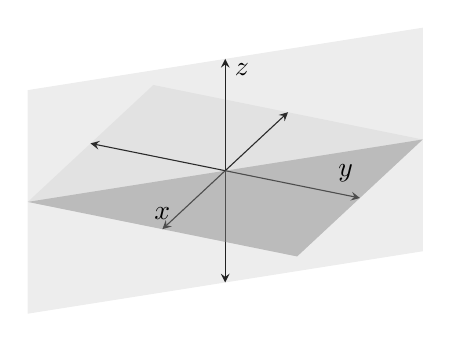
\begin{tikzpicture}
        \begin{axis}[width=6.6cm,height=6.6cm,
        xlabel=$y$, ylabel=\empty, zlabel=$z$,
        xmin=-4.9, xmax=4.9,
        ymin=-4.9, ymax=4.9,
        zmin=-4.9, zmax=4.9,
        axis lines=center,
        %xticklabel=\empty,
        %yticklabel=\empty,
        %zticklabel=\empty,
        axis line style={stealth-stealth},
        ticks=none,
        ]
            \fill[gray,opacity=0.1] (xyz cs:x=-4.9,y=-4.9,z=0) -- (xyz cs:x=4.9,y=-4.9,z=0) -- (xyz cs:x=4.9,y=4.9,z=0) --  (xyz cs:x=-4.9,y=4.9,z=0) -- cycle;
            \fill[gray!70,opacity=0.2] (xyz cs:x=-4.9,y=-4.9,z=-4.9) -- (xyz cs:x=4.9,y=4.9,z=-4.9) -- (xyz cs:x=4.9,y=4.9,z=4.9) --  (xyz cs:x=-4.9,y=-4.9,z=4.9) -- cycle;
            \fill[gray,opacity=0.4] (xyz cs:x=-4.9,y=-4.9,z=0) -- (xyz cs:x=4.9,y=-4.9,z=0) -- (xyz cs:x=4.9,y=4.9,z=0) -- cycle;
            \node at (0,-4.9,0.7) {$x$};
        \end{axis}
    \end{tikzpicture}
    }
    \begin{align*}
        H & = \left\{ \mathbb{x} \in \RR[3] \mid x + y + z = 0 \right\} \\
        & = \left\{ \begin{pmatrix}
            x \\
            y \\
            z
        \end{pmatrix} \in \RR[3] \mid z = -x-y \right\} \\
        & = \left\{ \begin{pmatrix}
            x \\
            y \\
            -x-y
        \end{pmatrix}; \, x, y \in \RR \right\} \\
        & = \left\{ \begin{pmatrix*}[r]
            x \\
            0 \\
            -x
        \end{pmatrix*} + \begin{pmatrix*}[r]
            0 \\
            y \\
            -y
        \end{pmatrix*}; \, x, y \in \RR \right\} \\
        & = \left\{ x \begin{pmatrix*}[r]
            1 \\
            0 \\
            -1
        \end{pmatrix*} + y \begin{pmatrix*}[r]
            0 \\
            1 \\
            -1
        \end{pmatrix*}; \, x, y \in \RR \right\} \\
        & = \Gen \left( \left\{ \begin{pmatrix*}[r]
            1 \\
            0 \\
            -1
        \end{pmatrix*}, \begin{pmatrix*}[r]
            0 \\
            1 \\
            -1
        \end{pmatrix*} \right\} \right)
    \end{align*}
    Además, observemos que el anterior conjunto de vectores es linealmente independientes. Por lo tanto, los vectores forman una base. Sea $\mathbb{v}_1 = \begin{pmatrix*}[r] 1 \\ 0 \\ -1 \end{pmatrix*}$ y $\mathbb{v}_2 = \begin{pmatrix*}[r] 0 \\ 1 \\ -1 \end{pmatrix*}$, aplicando el proceso de Gram-Schmidt con $\mathbb{u}_1 = \mathbb{v}_1$, obtenemos
    $$\hat{\mathbb{u}}_1 = \frac{1}{\sqrt{2}} \begin{pmatrix*}[r]
        1 \\
        0 \\
        -1
    \end{pmatrix*}$$
    Así, se sigue que
    \begin{align*}
        \mathbb{u}_2 & = \mathbb{v}_2 - (\mathbb{v}_2 \bullet \hat{\mathbb{u}}_1)\hat{\mathbb{u}}_1 \\
        & = \begin{pmatrix*}[r]
            0 \\
            1 \\
            -1
        \end{pmatrix*} - \frac{1}{2} \left[ \begin{pmatrix*}[r]
            0 \\
            1 \\
            -1
        \end{pmatrix*} \bullet \begin{pmatrix*}[r]
            1 \\
            0 \\
            -1
        \end{pmatrix*} \right] \begin{pmatrix*}[r]
            1 \\
            0 \\
            -1
        \end{pmatrix*} \\
        & = \begin{pmatrix*}[r]
            0 \\
            1 \\
            -1
        \end{pmatrix*} - \frac{1}{2}(1) \begin{pmatrix*}[r]
            1 \\
            0 \\
            -1
        \end{pmatrix*}
    \end{align*}
    Por lo tanto, $\mathbb{u}_2 = \begin{pmatrix*}[r]
        -1/2 \\
        1 \\
        -1/2
    \end{pmatrix*} = \dfrac{1}{2} \begin{pmatrix*}[r]
        -1 \\
        2 \\
        -1
    \end{pmatrix*}$. Es evidente que $\mathbb{u}_1$ y $\mathbb{u}_2$ son ortogonales y además,
    $$\hat{\mathbb{u}}_2 = \frac{1}{\sqrt{6}} \begin{pmatrix*}[r]
        -1 \\
        2 \\
        -1
    \end{pmatrix*}$$
    Así, $\displaystyle\left\{ \hat{\mathbb{u}}_1 = \frac{1}{\sqrt{2}} \begin{pmatrix*}[r]
        1 \\
        0 \\
        -1
    \end{pmatrix*}, \hat{\mathbb{u}}_2 = \frac{1}{\sqrt{6}} \begin{pmatrix*}[r]
        -1 \\
        2 \\
        -1
    \end{pmatrix*} \right\}$ es una base ortonormal de $H$. Finalmente,
    \begin{align*}
        \proy_H \mathbb{v} & = (\mathbb{v} \bullet \hat{\mathbb{u}}_1)\hat{\mathbb{u}}_1 + (\mathbb{v} \bullet \hat{\mathbb{u}}_2)\hat{\mathbb{u}}_2 \\
        & = \frac{1}{2} \left[ \begin{pmatrix}
            1 \\
            1 \\
            2
        \end{pmatrix} \bullet \begin{pmatrix*}[r]
            1 \\
            0 \\
            -1
        \end{pmatrix*} \right] \begin{pmatrix*}[r]
            1 \\
            0 \\
            -1
        \end{pmatrix*} + \frac{1}{6} \left[ \begin{pmatrix}
            1 \\
            1 \\
            2
        \end{pmatrix} \bullet \begin{pmatrix*}[r]
            -1 \\
            2 \\
            -1
        \end{pmatrix*} \right] \begin{pmatrix*}[r]
            -1 \\
            2 \\
            -1
        \end{pmatrix*} \\
        & = \frac{1}{2} \begin{pmatrix*}[r]
            -1 \\
            0 \\
            1
        \end{pmatrix*} + \frac{1}{6} \begin{pmatrix*}[r]
            1 \\
            -2 \\
            1
        \end{pmatrix*}
    \end{align*}
    Por lo tanto $\proy_H \mathbb{v} = \begin{pmatrix*}[r]
        -1/3 \\
        -1/3 \\
        2/3
    \end{pmatrix*} = \dfrac{1}{3} \begin{pmatrix*}[r]
        -1 \\
        -1 \\
        2
    \end{pmatrix*}$.
\end{example}

\section{Operadores ortogonales y sus matrices}

Los operadores ortogonales son transformaciones lineales que mantienen la longitud y los ángulos entre vectores en un espacio vectorial. Es decir, preservan la estructura geométrica del espacio en el que operan. En un espacio euclidiano, un operador lineal \( T \) se considera ortogonal si para cualquier par de vectores \( \mathbb{u} \) y \( \mathbb{v} \) en el espacio, el producto escalar de \( T\mathbb{u} \) y \( T\mathbb{v} \) es igual al producto escalar de \( \mathbb{u} \) y \( \mathbb{v} \).

\begin{definition}
    Sea $H \subseteq \RR[n]$ un subespacio de dimensión menor o igual a $n$ y sea $\left\{ \hat{\mathbb{u}}_1, \hat{\mathbb{u}}_2, \dots, \hat{\mathbb{u}}_k \right\}$ una base ortonormal de $H$. Sea $T: \RR[n] \longrightarrow H$ una transformación lineal definida como:
    $$T\mathbb{v} = (\mathbb{v} \bullet \hat{\mathbb{u}}_1)\hat{\mathbb{u}}_1 + (\mathbb{v} \bullet \hat{\mathbb{u}}_2)\hat{\mathbb{u}}_2 + \cdots + (\mathbb{v} \bullet \hat{\mathbb{u}}_k)\hat{\mathbb{u}}_k$$
    A esta transformación se le llamará \emph{transformación de proyección ortogonal}.
\end{definition}

\begin{observation}
    La transformación anteriormente mencionada es lineal. En efecto: Demostremos pues, que $T$ cumple las dos propiedades de la definición \ref{def:operatorlineal}.
    \begin{enumerate}[label=\roman*)]
        \item Sea $\mathbb{v}$, $\mathbb{w} \in \RR[n]$. Entonces
        \begin{align*}
            T(\mathbb{v} + \mathbb{w}) & = \big((\mathbb{v} + \mathbb{w}) \bullet \hat{\mathbb{u}}_1\big)\hat{\mathbb{u}}_1 + \big((\mathbb{v} + \mathbb{w}) \bullet \hat{\mathbb{u}}_2\big)\hat{\mathbb{u}}_2 + \cdots + \big((\mathbb{v} + \mathbb{w}) \bullet \hat{\mathbb{u}}_k\big)\hat{\mathbb{u}}_k \\
            & = (\mathbb{v} \bullet \hat{\mathbb{u}}_1 + \mathbb{w} \bullet \hat{\mathbb{u}}_1)\hat{\mathbb{u}}_1 + (\mathbb{v} \bullet \hat{\mathbb{u}}_2 + \mathbb{w} \bullet \hat{\mathbb{u}}_2)\hat{\mathbb{u}}_2 + \cdots + (\mathbb{v} \bullet \hat{\mathbb{u}}_k + \mathbb{w} \bullet \hat{\mathbb{u}}_k)\hat{\mathbb{u}}_k \\
            & = (\mathbb{v} \bullet \hat{\mathbb{u}}_1)\hat{\mathbb{u}}_1 + (\mathbb{w} \bullet \hat{\mathbb{u}}_1)\hat{\mathbb{u}}_1 + (\mathbb{v} \bullet \hat{\mathbb{u}}_2)\hat{\mathbb{u}}_2 + (\mathbb{w} \bullet \hat{\mathbb{u}}_2)\hat{\mathbb{u}}_2 + \cdots + (\mathbb{v} \bullet \hat{\mathbb{u}}_k)\hat{\mathbb{u}}_k + (\mathbb{w} \bullet \hat{\mathbb{u}}_k)\hat{\mathbb{u}}_k \\
            & = (\mathbb{v} \bullet \hat{\mathbb{u}}_1)\hat{\mathbb{u}}_1 + (\mathbb{v} \bullet \hat{\mathbb{u}}_2)\hat{\mathbb{u}}_2 + \cdots + (\mathbb{v} \bullet \hat{\mathbb{u}}_k)\hat{\mathbb{u}}_k + (\mathbb{w} \bullet \hat{\mathbb{u}}_1)\hat{\mathbb{u}}_1 + (\mathbb{w} \bullet \hat{\mathbb{u}}_2)\hat{\mathbb{u}}_2 + \cdots + (\mathbb{w} \bullet \hat{\mathbb{u}}_k)\hat{\mathbb{u}}_k \\
            & = T\mathbb{v} + T\mathbb{w}
        \end{align*}
        Por lo tanto, $T(\mathbb{v} + \mathbb{w}) = T\mathbb{v} + T\mathbb{w}$.
        \item Sea $\mathbb{v} \in \RR[n]$ y $\alpha \in \RR$. Entonces
        \begin{align*}
            T(\alpha \mathbb{v}) & = \big((\alpha \mathbb{v}) \bullet \hat{\mathbb{u}}_1\big)\hat{\mathbb{u}}_1 + \big((\alpha \mathbb{v}) \bullet \hat{\mathbb{u}}_2\big)\hat{\mathbb{u}}_2 + \cdots + \big((\alpha \mathbb{v}) \bullet \hat{\mathbb{u}}_k\big)\hat{\mathbb{u}}_k \\
            & = \big(\alpha (\mathbb{v} \bullet \hat{\mathbb{u}}_1)\big)\hat{\mathbb{u}}_1 + \big(\alpha (\mathbb{v} \bullet \hat{\mathbb{u}}_2)\big)\hat{\mathbb{u}}_2 + \cdots + \big(\alpha (\mathbb{v} \bullet \hat{\mathbb{u}}_k)\big)\hat{\mathbb{u}}_k \\
            & = \alpha \big((\mathbb{v} \bullet \hat{\mathbb{u}}_1)\hat{\mathbb{u}}_1 + (\mathbb{v} \bullet \hat{\mathbb{u}}_2)\hat{\mathbb{u}}_2 + \cdots + (\mathbb{v} \bullet \hat{\mathbb{u}}_k)\hat{\mathbb{u}}_k\big) \\
            & = \alpha T\mathbb{v}
        \end{align*}
        Por lo tanto, $T(\alpha \mathbb{v}) = \alpha T\mathbb{v}$.
    \end{enumerate}
    De (i) y (ii), se sigue que $T$ es lineal.
\end{observation}

\begin{theorem}\label{BAHJQGGGFFDQFXXFHZHAHQGYQ}
    Sea $\mathbb{v} \in \RR[n]$ y $\left\{ \hat{\mathbb{u}}_1, \hat{\mathbb{u}}_2, \dots, \hat{\mathbb{u}}_n \right\}$ una base ortonormal de $\RR[n]$, entonces
    $$\mathbb{v} = (\mathbb{v} \bullet \hat{\mathbb{u}}_1)\hat{\mathbb{u}}_1 + (\mathbb{v} \bullet \hat{\mathbb{u}}_2)\hat{\mathbb{u}}_2 + \cdots + (\mathbb{v} \bullet \hat{\mathbb{u}}_n)\hat{\mathbb{u}}_n$$
    \demostracion Dado que $\mathbb{v} \in \RR[n]$, entonces podemos expresarlo como una combinación lineal de la base ortonormal $\left\{ \hat{\mathbb{u}}_1, \hat{\mathbb{u}}_2, \dots, \hat{\mathbb{u}}_n \right\}$, es decir,
    \begin{equation}
        \mathbb{v} = a_1\hat{\mathbb{u}}_1 + a_2\hat{\mathbb{u}}_2 + \cdots + a_n\hat{\mathbb{u}}_n \label{CYA}
    \end{equation}
    donde $a_i \in \RR$. Además, se cumple que
    $$\hat{\mathbb{u}}_i \bullet \hat{\mathbb{u}}_j = \begin{cases}
        1 & \text{ si } i = j \\
        0 & \text{ si } i \neq j
    \end{cases} \qquad \text{para } i, j = 1, 2, \dots, n$$
    Por lo tanto,
    \begin{align*}
        \hat{\mathbb{u}}_i \bullet \mathbb{v} & = \hat{\mathbb{u}}_i \bullet \left( a_1\hat{\mathbb{u}}_1 + a_2\hat{\mathbb{u}}_2 + \cdots + a_i\hat{\mathbb{u}}_i + \cdots + a_n\hat{\mathbb{u}}_n \right) \\
        & = \hat{\mathbb{u}}_i \bullet (a_1 \hat{\mathbb{u}}_1) + \hat{\mathbb{u}}_i \bullet (a_2 \hat{\mathbb{u}}_2) + \cdots + \hat{\mathbb{u}}_i \bullet (a_i \hat{\mathbb{u}}_i) + \cdots + \hat{\mathbb{u}}_i \bullet (a_n \hat{\mathbb{u}}_n) \\
        & = a_1(\hat{\mathbb{u}}_i \bullet \hat{\mathbb{u}}_1) + a_2(\hat{\mathbb{u}}_i \bullet \hat{\mathbb{u}}_2) + \cdots + a_i(\hat{\mathbb{u}}_i \bullet \hat{\mathbb{u}}_i) + \cdots + a_n(\hat{\mathbb{u}}_i \bullet \hat{\mathbb{u}}_n) \\
        & = a_1 \cdot 0 + a_2 \cdot 0 + \cdots + a_i(\hat{\mathbb{u}}_i \bullet \hat{\mathbb{u}}_i) + \cdots + a_n \cdot 0 \\
        & = a_i(\hat{\mathbb{u}}_i \bullet \hat{\mathbb{u}}_i)
    \end{align*}
    Así que,
    $$\hat{\mathbb{u}}_i \bullet \mathbb{v} = a_i(\hat{\mathbb{u}}_i \bullet \hat{\mathbb{u}}_i)$$
    lo que implica que
    $$a_i = \hat{\mathbb{u}}_i \bullet \mathbb{v}$$
    Sustituyendo en la expresión \eqref{CYA}, se obtiene que
    $$\mathbb{v} = (\mathbb{v} \bullet \hat{\mathbb{u}}_1)\hat{\mathbb{u}}_1 + (\mathbb{v} \bullet \hat{\mathbb{u}}_2)\hat{\mathbb{u}}_2 + \cdots + (\mathbb{v} \bullet \hat{\mathbb{u}}_n)\hat{\mathbb{u}}_n$$
\end{theorem}

\begin{observation}
    En otras palabras, el teorema anterior nos dice que cualquier vector $\mathbb{v}$ en $\RR[n]$ puede ser expresado como la suma de sus proyecciones sobre los vectores unitarios de una base ortonormal $\hat{\mathbb{u}}_1, \hat{\mathbb{u}}_2, \dots, \hat{\mathbb{u}}_n$, multiplicados por dichos vectores unitarios. Esencialmente, descompone el vector $\mathbb{v}$ en componentes a lo largo de cada dirección representada por los vectores unitarios de la base.
\end{observation}

\newpage

\begin{example}
    La notación \( e_1, e_2, e_3 \) se utiliza comúnmente para denotar los vectores de la base canónica en \( \RR[3] \). Sin embargo, es perfectamente válido y frecuente utilizar la notación \( \hat{\imath}, \hat{\jmath}, \hat{k} \) para representar los vectores unitarios en el espacio tridimensional \( \RR[3] \). Consideremos la base ortonotmal $\{ e_1, e_2, e_3 \}$ en $\RR[3]$. Sea $\mathbb{v} \in \RR[3]$ con $\mathbb{v} = \begin{pmatrix} x \\ y \\ z \end{pmatrix}$, por el teorema anterior
    \begin{align*}
        \mathbb{v} & = (\mathbb{v} \bullet e_1)e_1 + (\mathbb{v} \bullet e_2)e_2 + (\mathbb{v} \bullet e_3)e_3 \\
        & = \left[ \begin{pmatrix} x \\ y \\ z \end{pmatrix} \bullet \begin{pmatrix} 1 \\ 0 \\ 0 \end{pmatrix} \right] \hat{\imath} + \left[ \begin{pmatrix} x \\ y \\ z \end{pmatrix} \bullet \begin{pmatrix} 0 \\ 1 \\ 0 \end{pmatrix} \right] \hat{\jmath} + \left[ \begin{pmatrix} x \\ y \\ z \end{pmatrix} \bullet \begin{pmatrix} 0 \\ 0 \\ 1 \end{pmatrix} \right] \hat{k} \\
        & = x\hat{\imath} + y\hat{\jmath} + z\hat{k}
    \end{align*}
    Esta notación puede resultar intuitiva y práctica en contextos que involucren geometría tridimensional y física. La elección entre \( e_1, e_2, e_3 \) y \( \hat{\imath}, \hat{\jmath}, \hat{k} \) es en gran medida una cuestión de preferencia y conveniencia. Ambas notaciones son aceptadas y ampliamente reconocidas en el ámbito del álgebra lineal y la geometría.
\end{example}

Cuando se trabaja con operadores ortogonales, es común representarlos mediante matrices ortogonales.
\begin{definition}\label{def:matrixortogonal}
    Una matriz ortogonal es una matriz cuadrada cuya inversa es igual a su transpuesta. Es decir, una matriz $Q \in \mathcal{M}_{n \times n}(\RR)$ se llama ortogonal si $Q$ es invertible y $Q^{-1} = Q^T$. Formalmente, una matriz \( Q \) se considera ortogonal si cumple con la siguiente propiedad:\infoBulle{Las matrices ortogonales son importantes en muchas áreas, incluyendo geometría, transformaciones lineales y procesamiento de señales. Por ejemplo, las matrices de rotación y reflexión son ejemplos típicos de matrices ortogonales. Estas matrices conservan la norma euclidiana y la ortogonalidad entre vectores, lo que las hace fundamentales en diversas aplicaciones matemáticas y computacionales.}
    \[ Q^T Q = I_n \]
\end{definition}

\begin{theorem}\label{Qorto_vectoresorto}
    Dada $Q \in \mathcal{M}_{n \times n}(\RR)$. Entonces $Q$ es ortogonal si y solo si sus vectores columnas son ortonormales. \\
    \demostracion Sea
    $$Q = \begin{bmatrix}
        q_{11} & q_{12} & \cdots & q_{1n} \\
        q_{21} & q_{22} & \cdots & q_{2n} \\
        \vdots & & \ddots & \\
        q_{n1} & q_{n2} & \cdots & q_{nn}
    \end{bmatrix}$$
    entonces
    $$Q^T = \begin{bmatrix}
        q_{11} & q_{21} & \cdots & q_{n1} \\
        q_{21} & q_{22} & \cdots & q_{n2} \\
        \vdots & & \ddots & \\
        q_{1n} & q_{2n} & \cdots & q_{nn}
    \end{bmatrix}$$
    De manera análoga, sea
    $$\mathbb{q}_j = \begin{pmatrix}
        q_{1j} \\
        q_{2j} \\
        \vdots \\
        q_{nj}
    \end{pmatrix}$$
    entonces
    $$\mathbb{q}_j^t = (q_{1j}, q_{2j}, \dots, q_{nj})$$
    Así,
    $$Q^TQ = \begin{bmatrix}
        \mathbb{q}_1^t \mathbb{q}_1 & \mathbb{q}_1^t \mathbb{q}_2 & \cdots & \mathbb{q}_1^t \mathbb{q}_n \\
        \mathbb{q}_2^t \mathbb{q}_1 & \mathbb{q}_2^t \mathbb{q}_2 & \cdots & \mathbb{q}_2^t \mathbb{q}_n \\
        \vdots & & \ddots & \\
        \mathbb{q}_n^t \mathbb{q}_1 & \mathbb{q}_n^t \mathbb{q}_2 & \cdots & \mathbb{q}_n^t \mathbb{q}_n
    \end{bmatrix}$$\newpage\noindent
    pero por la observación \ref{Obs:innerproduct}, se sigue que
    \begin{equation}
        Q^TQ = \begin{bmatrix}
            \mathbb{q}_1 \bullet \mathbb{q}_1 & \mathbb{q}_1 \bullet \mathbb{q}_2 & \cdots & \mathbb{q}_1 \bullet \mathbb{q}_n \\
            \mathbb{q}_2 \bullet \mathbb{q}_1 & \mathbb{q}_2 \bullet \mathbb{q}_2 & \cdots & \mathbb{q}_2 \bullet \mathbb{q}_n \\
            \vdots & & \ddots & \\
            \mathbb{q}_n \bullet \mathbb{q}_1 & \mathbb{q}_n \bullet \mathbb{q}_2 & \cdots & \mathbb{q}_n \bullet \mathbb{q}_n
        \end{bmatrix} \label{JAJAJAJJABAJQJA}
    \end{equation}
    Supongamos que $Q$ es ortogonal, de la definición \ref{def:matrixortogonal}, tenemos que
    $$Q^T = Q^{-1}$$
    es decir,
    \begin{equation}
        Q^T Q = I_n \label{JAJAJJAKAnjak}
    \end{equation}
    De \eqref{JAJAJAJJABAJQJA} y \eqref{JAJAJJAKAnjak}, se sigue que
    $$Q^TQ = \begin{bmatrix}
        \| \mathbb{q}_1 \|^2 & \mathbb{q}_1 \bullet \mathbb{q}_2 & \cdots & \mathbb{q}_1 \bullet \mathbb{q}_n \\
        \mathbb{q}_2 \bullet \mathbb{q}_1 & \| \mathbb{q}_2 \|^2 & \cdots & \mathbb{q}_2 \bullet \mathbb{q}_n \\
        \vdots & & \ddots & \\
        \mathbb{q}_n \bullet \mathbb{q}_1 & \mathbb{q}_n \bullet \mathbb{q}_2 & \cdots & \| \mathbb{q}_n \|^2
    \end{bmatrix} = \begin{bmatrix}
        1 & 0 & \cdots & 0 \\
        0 & 1 & \cdots & 0 \\
        \vdots & & \ddots & \\
        0 & 0 & \cdots & 1
    \end{bmatrix}$$
    si y solo si
    $$\mathbb{q}_i \bullet \mathbb{q}_j = \begin{cases}
        1 & \text{ si } i = j \\
        0 & \text{ si } i \neq j
    \end{cases} \qquad \text{para } i, j = 1, 2, \dots, n$$
    si y solo si $\left\{ \mathbb{q}_1, \mathbb{q}_2, \dots, \mathbb{q}_n \right\}$ es ortonormal.
\end{theorem}

\begin{theorem}
    Sean $A \in \mathcal{M}_{n \times n}(\RR)$, $\mathbb{x} \in \RR[n]$ y $\mathbb{y} \in \RR[n]$. Entonces
    $$(A \mathbb{x}) \bullet \mathbb{y} = \mathbb{x} \bullet \left(A^T \mathbb{y}\right)$$
    \demostracion Consideremos a \( A \in \mathcal{M}_{n \times n}(\RR) \), \( \mathbb{x} \in \RR[n] \), y \( \mathbb{y} \in \RR[n] \). Entonces, la anterior relación puede ser demostrada fácilmente utilizando la observación \ref{Obs:innerproduct} y el teorema \ref{theo:matrixtranspu}. Por lo tanto,
    \begin{align*}
        (A\mathbb{x}) \bullet \mathbb{y} & = (A\mathbb{x})^T \mathbb{y} \\
        & = \left( \mathbb{x}^t A^T \right) \mathbb{y} \\
        & = \mathbb{x}^t \left(A^T \mathbb{y} \right) \\
        & = \mathbb{x} \bullet \left( A^T \mathbb{y} \right)
    \end{align*}
\end{theorem}

\begin{definition}
    Sea $Q \in \mathcal{M}_{n \times n}(\RR)$ y $T:\RR[n] \longrightarrow \RR[n]$ una transformación lineal definida como
    $$T\mathbb{x} = Q\mathbb{x}$$
    esto es
    \begin{align*}
        T: \RR[n] & \longrightarrow \RR[n] \\
        \mathbb{x} & \longmapsto T\mathbb{x} = Q\mathbb{x}
    \end{align*}
    A $T$ se le llama \emph{transformación lineal ortogonal} o simplemente \emph{transformación ortogonal}.
\end{definition}

\begin{observation}
    Observe que de la anterior definición, se sigue que
    \begin{align*}
        (T\mathbb{x}) \bullet (T\mathbb{x}) & = (Q\mathbb{x}) \bullet (Q\mathbb{x}) \\
        & = \mathbb{x} \bullet \left( Q^T Q \mathbb{x} \right) \\
        & = \mathbb{x} \bullet (I_n \mathbb{x}) \\
        & = \mathbb{x} \bullet \mathbb{x}
    \end{align*}
    Esto es
    $$(T\mathbb{x}) \bullet (T\mathbb{x}) = \mathbb{x} \bullet \mathbb{x}$$
    entonces $\| T\mathbb{x} \|^2 = \| \mathbb{x} \|^2$ de donde de sigue que $\| T\mathbb{x} \| = \| \mathbb{x} \|$.
\end{observation}

\newpage

\begin{definition}
    Sea $T:\RR[n] \longrightarrow \RR[n]$ una transformación lineal. Decimos que $T$ es una isometría si $\| T\mathbb{x} \| = \| \mathbb{x} \|$.
\end{definition}

En otras palabras, una isometría es una transformación lineal que preserva las distancias entre puntos en un espacio vectorial. Es decir, si tienes dos puntos \( \mathbb{v} \) y \( \mathbb{w} \) en un espacio vectorial \( V \), la distancia entre ellos antes y después de aplicar la isometría es la misma.

Formalmente, una transformación lineal \( T: V \longrightarrow W \) entre dos espacios vectoriales \( V \) y \( W \) con productos internos (o normas) respectivamente, es una isometría si para todos los vectores \( \mathbb{v}_1 \) y \( \mathbb{v}_2 \) en \( V \), se cumple que:
$$\|T\mathbb{v}_1 - T\mathbb{v}_2\| = \|\mathbb{v}_1 - \mathbb{v}_2\|$$
Esto significa que la norma de la diferencia entre los vectores transformados es igual a la norma de la diferencia entre los vectores originales.

Las isometrías son importantes porque conservan la estructura geométrica de los espacios vectoriales. Algunos ejemplos comunes de isometrías incluyen rotaciones, reflexiones y traslaciones en el espacio euclidiano tridimensional.

\begin{theorem}\label{YAYYYYQYQYAYGGFCXXZSSS}
    Sea $T:\RR[n] \longrightarrow \RR[n]$ una isometría, entonces
    $$(T\mathbb{x}) \bullet (T\mathbb{y}) = \mathbb{x} \bullet \mathbb{y}$$
    \demostracion Considere
    \begin{align*}
        \| T\mathbb{x} - T\mathbb{y} \|^2 & = (T\mathbb{x} - T\mathbb{y}) \bullet (T\mathbb{x} - T\mathbb{y}) \\
        & = (T\mathbb{x} - T\mathbb{y}) \bullet (T\mathbb{x}) - (T\mathbb{x} - T\mathbb{y}) \bullet (T\mathbb{y}) \\
        & = (T\mathbb{x}) \bullet (T\mathbb{x}) - (T\mathbb{x}) \bullet (T\mathbb{y}) - (T\mathbb{x}) \bullet (T\mathbb{y}) + (T\mathbb{y}) \bullet (T\mathbb{y}) \\
        & = \| \mathbb{x} \|^2 - 2(T\mathbb{x}) \bullet (T\mathbb{y}) + \| \mathbb{y} \|^2
    \end{align*}
    Es decir,
    \begin{equation}
        \| T\mathbb{x} - T\mathbb{y} \|^2 = \| \mathbb{x} \|^2 - 2(T\mathbb{x}) \bullet (T\mathbb{y}) + \| \mathbb{y} \|^2 \label{CONST1}
    \end{equation}
    De manera análoga,
    \begin{align*}
        \| \mathbb{x} - \mathbb{y} \|^2 & = (\mathbb{x} - \mathbb{y}) \bullet (\mathbb{x} - \mathbb{y}) \\
        & = (\mathbb{x} - \mathbb{y}) \bullet (\mathbb{x}) - (\mathbb{x} - \mathbb{y}) \bullet (\mathbb{y}) \\
        & = \mathbb{x} \bullet \mathbb{x} - \mathbb{x} \bullet \mathbb{y} - \mathbb{x} \bullet \mathbb{y} + \mathbb{y} \bullet \mathbb{y} \\
        & = \| \mathbb{x} \|^2 - 2(\mathbb{x} \bullet \mathbb{y}) + \| \mathbb{y} \|^2
    \end{align*}
    Es decir,
    \begin{equation}
        \| \mathbb{x} - \mathbb{y} \|^2 = \| \mathbb{x} \|^2 - 2(\mathbb{x} \bullet \mathbb{y}) + \| \mathbb{y} \|^2 \label{CONST2}
    \end{equation}
    Luego, por ser $T$ una isometría y lineal, se sigue que
    \begin{equation}
        \| T\mathbb{x} - T\mathbb{y} \| = \| \mathbb{x} - \mathbb{y} \| \label{CONST3}
    \end{equation}
    Sustituyendo \eqref{CONST1} y \eqref{CONST2} en \eqref{CONST3}, se obtiene que
    $$\| \mathbb{x} \|^2 - 2(T\mathbb{x}) \bullet (T\mathbb{y}) + \| \mathbb{y} \|^2 = \| \mathbb{x} \|^2 - 2(\mathbb{x} \bullet \mathbb{y}) + \| \mathbb{y} \|^2$$
    de donde se sigue que $(T\mathbb{x}) \bullet (T\mathbb{y}) = \mathbb{x} \bullet \mathbb{y}$.
\end{theorem}

\begin{definition}
    Sea $H$ un subespacio de $\RR[n]$. El complemento ortogonal de $H$, denotado por $H^{\bot}$, se define como
    $$H^{\bot} = \left\{ \mathbb{x} \in \RR[n] \mid \mathbb{x} \bullet \mathbb{h} = 0, \text{ para toda } \mathbb{h} \in H \right\}$$
\end{definition}

\begin{example}
    Consideremos $\RR[2]$ y sea $H = \left\{ \mathbb{x} \in \RR[2] \mid y = 2x \right\}$. Determinemos $H^{\bot}$, es decir, deseamos encontrar
    \begin{equation}
        H^{\bot} = \left\{ \begin{pmatrix} x' \\ y' \end{pmatrix} \in \RR[2] \mid \begin{pmatrix} x' \\ y' \end{pmatrix} \bullet \mathbb{h} = 0, \text{ para toda } \mathbb{h} \in H \right\} \label{JAJSJSJSJSJDJDJGYYGQG}
    \end{equation}\newpage\noindent
    De esta manera,
    \begin{align*}
        H & = \left\{ \begin{pmatrix} x \\ y \end{pmatrix} \in \RR[2] \mid y = 2x \right\} \\
        & = \left\{ \begin{pmatrix} x \\ 2 x \end{pmatrix}, x \in \RR \right\} \\
        & = \left\{ x \begin{pmatrix} 1 \\ 2 \end{pmatrix}, x \in \RR \right\}
    \end{align*}
    Así, $H = \Gen \left( \left\{ \begin{pmatrix} 1 \\ 2 \end{pmatrix} \right\} \right)$. De esta forma, $\mathbb{h} \in H$ está dada por
    $$\mathbb{h} = \alpha \begin{pmatrix} 1 \\ 2 \end{pmatrix}, \text{ con } \alpha \in \RR$$
    Sustituyendo en \eqref{JAJSJSJSJSJDJDJGYYGQG}, se sigue que\sideFigure[]{
    \begin{tikzpicture}
        \draw[-stealth] (-2.5,0) -- (2.5,0) node[below left] {$x$};
        \draw[-stealth] (0,-2.5) -- (0,2.5) node[below left] {$y$};
        \draw[latex-latex] (1,2) -- (0,0) -- (1,-0.5);
        \draw[dash pattern=on 3pt off 3pt] (-1.25,-2.5) -- (1.25,2.5) node[below right] {$H$};
        \draw[dash pattern=on 3pt off 3pt] (-2.5,1.25) -- (2.5,-1.25) node[below left] {$H^{\bot}$};
    \end{tikzpicture}
    }
    \begin{align*}
        H^{\bot} & = \left\{ \begin{pmatrix} x' \\ y' \end{pmatrix} \in \RR[2] \mid \begin{pmatrix} x' \\ y' \end{pmatrix} \bullet \left( \alpha \begin{pmatrix} 1 \\ 2 \end{pmatrix} \right) = 0, \text{ para todo } \alpha \in \RR \right\} \\
        & = \left\{ \begin{pmatrix} x' \\ y' \end{pmatrix} \in \RR[2] \mid \alpha (x' + 2y') = 0, \text{ para todo } \alpha \in \RR \right\} \\
        & = \left\{ \begin{pmatrix} x' \\ y' \end{pmatrix} \in \RR[2] \mid x' + 2y' = 0 \right\} \\
        & = \left\{ \begin{pmatrix} x' \\ y' \end{pmatrix} \in \RR[2] \mid y' = -1/2 x' \right\} \\
        & = \left\{ \begin{pmatrix*}[r] x' \\ -1/2 x' \end{pmatrix*}, x \in \RR \right\} \\
        & = \left\{ x' \begin{pmatrix*}[r] 1 \\ -1/2 \end{pmatrix*}, x \in \RR \right\}
    \end{align*}
    Por lo tanto, $H^{\bot} = \Gen \left( \left\{ \begin{pmatrix*}[r] 1 \\ -1/2 \end{pmatrix*} \right\} \right)$.
\end{example}

\begin{theorem}\label{tres_teoremas_fuertes}
    Sea $H$ un subespacio de $\RR[n]$, entonces
    \begin{enumerate}[label=\roman*)]
        \item $H^{\bot}$ es subespacio de $\RR[n]$.
        \item $H \cap H^{\bot} = \{ \mathbb{0} \}$.
        \item $\Dim H^{\bot} = n - \Dim H$.
    \end{enumerate}
    \demostracion
    \begin{enumerate}[label=\roman*)]
        \item Para probar que $H^{\bot}$ es subespacio de $\RR[n]$, debemos probar que $H^{\bot}$ cumple los dos axiomas de cerradura. Sean $\mathbb{x}$, $\mathbb{y} \in H^{\bot}$, entonces
        $$\mathbb{x} \bullet \mathbb{h} = 0, \text{ para toda } \mathbb{h} \in H$$
        e
        $$\mathbb{y} \bullet \mathbb{h} = 0, \text{ para toda } \mathbb{h} \in H$$
        Así
        \begin{align*}
            (\mathbb{x} + \mathbb{y}) \bullet \mathbb{h} & = \mathbb{x} \bullet \mathbb{h} + \mathbb{y} \bullet \mathbb{h} \\
            & = 0 + 0 \\
            & = 0
        \end{align*}
        Por lo tanto, $\mathbb{x} + \mathbb{y} \in H^{\bot}$. De manera análoga, sean $\mathbb{x} \in H^{\bot}$ y $\alpha \in \RR$, entonces
        \begin{align*}
            (\alpha \mathbb{x}) \bullet \mathbb{h} & = \alpha (\mathbb{x} \bullet \mathbb{h}) \\
            & = \alpha \cdot 0 \\
            & = 0
        \end{align*}
        En consecuencia, $\alpha \mathbb{x} \in H^{\bot}$. Dado que se cumplen ambas propiedades de cerradura, se concluye que $H^{\bot}$ es un subespacio de $\RR[n]$.
        \item Sea $\mathbb{x} \in H \cap H^{\bot} \Longrightarrow \mathbb{x} \in H$ \& $\mathbb{x} \in H^{\bot} \Longrightarrow \mathbb{x} \in H$ \& $\mathbb{x} \bullet \mathbb{h} = 0$, para toda $\mathbb{h} \in H$. Específicamente, esto se cumple cuando $\mathbb{h}$ es igual a $\mathbb{x}$, lo que resulta en $\mathbb{x} \bullet \mathbb{x} = 0$ o, equivalentemente, $\| \mathbb{x} \|^2 = 0$. Según la proposición \ref{prop:norma}, se concluye que $\mathbb{x} = \mathbb{0}$. Por lo tanto, $H \cap H^{\bot} = \{ \mathbb{0} \}$.
        \item Sea $H$ un subespacio de $\RR[n]$ y sea $\left\{ \hat{\mathbb{u}}_1, \hat{\mathbb{u}}_2, \dots, \hat{\mathbb{u}}_n \right\}$ una base ortonormal de $\RR[n]$, siendo
        $$\hat{\mathbb{u}}_i \bullet \hat{\mathbb{u}}_j = \begin{cases}
            1 & \text{ si } i = j \\
            0 & \text{ si } i \neq j
        \end{cases} \qquad \text{para } i, j = 1, 2, \dots, n$$
        Dado que $H \subseteq \RR[n]$, supongamos que $H = \Gen \left( \left\{ \hat{\mathbb{u}}_1, \hat{\mathbb{u}}_2, \dots, \hat{\mathbb{u}}_k \right\} \right)$ con $k \leq n$, así que asumimos que
        $$H^{\bot} = \Gen \left( \left\{ \hat{\mathbb{u}}_{k+1}, \hat{\mathbb{u}}_{k+2}, \dots, \hat{\mathbb{u}}_n \right\} \right)$$
        Así pues, demostremos que, en efecto, es cierto lo anterior. Sea $\mathbb{w}$ un elemento de $H^{\bot}$, entonces
        $$\mathbb{w} = \beta_{k+1} \hat{\mathbb{u}}_{k+1} + \beta_{k+2} \hat{\mathbb{u}}_{k+2} + \cdots + \beta_n \hat{\mathbb{u}}_n$$
        Ahora, sea $\mathbb{h} \in H$, entonces
        $$\mathbb{h} = \alpha_1 \hat{\mathbb{u}}_1 + \alpha_2 \hat{\mathbb{u}}_2 + \cdots + \alpha_k \hat{\mathbb{u}}_n$$
        Así, se sigue que
        \begin{align*}
            \mathbb{w} \bullet \mathbb{h} & = \left( \beta_{k+1} \hat{\mathbb{u}}_{k+1} + \beta_{k+2} \hat{\mathbb{u}}_{k+2} + \cdots + \beta_n \hat{\mathbb{u}}_n \right) \bullet \left( \alpha_1 \hat{\mathbb{u}}_1 + \alpha_2 \hat{\mathbb{u}}_2 + \cdots + \alpha_k \hat{\mathbb{u}}_n \right) \\
            & = \beta_{k+1} \alpha_1 (\hat{\mathbb{u}}_{k+1} \bullet \hat{\mathbb{u}}_1) + \beta_{k+1} \alpha_2 (\hat{\mathbb{u}}_{k+1} \bullet \hat{\mathbb{u}}_2) + \cdots + \beta_{k+1} \alpha_k (\hat{\mathbb{u}}_{k+1} \bullet \hat{\mathbb{u}}_k) \\
            & \qquad \beta_{k+2} \alpha_1 (\hat{\mathbb{u}}_{k+2} \bullet \hat{\mathbb{u}}_1) + \beta_{k+2} \alpha_2 (\hat{\mathbb{u}}_{k+2} \bullet \hat{\mathbb{u}}_2) + \cdots + \beta_{k+2} \alpha_k (\hat{\mathbb{u}}_{k+2} \bullet \hat{\mathbb{u}}_k) \\
            & \qquad\qquad + \cdots + \beta_{n} \alpha_1 (\hat{\mathbb{u}}_{n} \bullet \hat{\mathbb{u}}_1) + \beta_{n} \alpha_2 (\hat{\mathbb{u}}_{n} \bullet \hat{\mathbb{u}}_2) + \cdots + \beta_{n} \alpha_k (\hat{\mathbb{u}}_{n} \bullet \hat{\mathbb{u}}_k) \\
            & = 0
        \end{align*}
        Por lo tanto, $H^{\bot} = \Gen \left( \left\{ \hat{\mathbb{u}}_{k+1}, \hat{\mathbb{u}}_{k+2}, \dots, \hat{\mathbb{u}}_n \right\} \right)$ sí es el complemento ortogonal de $H$. De esta forma,
        \begin{align*}
            \Dim H + \Dim H^{\bot} & = k + (n - k) \\
            & = n
        \end{align*}
        Por lo tanto, $\Dim H^{\bot} = n - \Dim H$.
    \end{enumerate}
\end{theorem}

\begin{theorem}\label{suma_proyecciones}
    Sea $H$ un subespacio de $\RR[n]$ y sea $\mathbb{v} \in \RR[n]$. Entonces existe un par único de vectores $\mathbb{h} \in H$ y $\mathbb{k} \in H^{\bot}$ tales que
    $$\mathbb{v} = \mathbb{h} + \mathbb{k}$$
    Más aún,
    $$\mathbb{v} = \proy_{H}\mathbb{v} + \proy_{H^{\bot}}\mathbb{v}$$
    \demostracion Sea $\left\{ \hat{\mathbb{u}}_1, \hat{\mathbb{u}}_2, \dots, \hat{\mathbb{u}}_n \right\}$ una base ortonormal de $\RR[n]$. Por el teorema \ref{BAHJQGGGFFDQFXXFHZHAHQGYQ}, tenemos que
    \begin{align*}
        \mathbb{v} & = (\mathbb{v} \bullet \hat{\mathbb{u}}_1)\hat{\mathbb{u}}_1 + (\mathbb{v} \bullet \hat{\mathbb{u}}_2)\hat{\mathbb{u}}_2 + \cdots + (\mathbb{v} \bullet \hat{\mathbb{u}}_n)\hat{\mathbb{u}}_n \\
        & = (\mathbb{v} \bullet \hat{\mathbb{u}}_1)\hat{\mathbb{u}}_1 + (\mathbb{v} \bullet \hat{\mathbb{u}}_2)\hat{\mathbb{u}}_2 + \cdots + (\mathbb{v} \bullet \hat{\mathbb{u}}_k)\hat{\mathbb{u}}_k + (\mathbb{v} \bullet \hat{\mathbb{u}}_{k+1})\hat{\mathbb{u}}_{k+1} + (\mathbb{v} \bullet \hat{\mathbb{u}}_{k+2})\hat{\mathbb{u}}_{k+2} + \cdots + (\mathbb{v} \bullet \hat{\mathbb{u}}_n)\hat{\mathbb{u}}_n \\
        & = \proy_{H}\mathbb{v} + \proy_{H^{\bot}}\mathbb{v} \\
        & = \mathbb{h} + \mathbb{k}
    \end{align*}
    siendo $\mathbb{h} = \proy_{H}\mathbb{v}$ y $\mathbb{k} = \proy_{H^{\bot}}\mathbb{v}$.
\end{theorem}

\begin{theorem}[Teorema de aproximación de la norma]\label{theo:aproxnorma}
    Sea $H$ un subespacio de $\RR[n]$ y sea $\mathbb{v}$ un vector en $\RR[n]$. Entonces $\proy_{H}\mathbb{v}$ es la mejor aproximación para $\mathbb{v}$ en $H$ en el siguiente sentido: si $\mathbb{h}$ es cualquier otro vector en $H$, entonces
    $$\| \mathbb{v} - \proy_{H}\mathbb{v} \| < \| \mathbb{v} - \mathbb{h} \|$$\newpage
    \demostracion Del teorema anterior, tenemos que $\mathbb{v} - \proy_{H} \mathbb{v} \in H^{\bot}$. Así, podemos escribir
    $$\mathbb{v} - \mathbb{h} = (\mathbb{v} - \proy_{H}\mathbb{v}) + (\proy_{H}\mathbb{v} - \mathbb{h})$$
    El primer término de la derecha está en $H^{\bot}$, mientras que el segundo está en $H$. De esta forma,
    $$(\mathbb{v} - \proy_{H}\mathbb{v}) \bullet (\proy_{H}\mathbb{v} - \mathbb{h}) = 0$$
    Así pues, se sigue que
    \begin{align*}
        \| \mathbb{v} - \mathbb{h} \|^2 & = (\mathbb{v} - \proy_{H}\mathbb{v}) \bullet (\proy_{H}\mathbb{v} - \mathbb{h}) \\
        & = [(\mathbb{v} - \proy_{H}\mathbb{v}) + (\proy_{H}\mathbb{v} - \mathbb{h})] \bullet [(\mathbb{v} - \proy_{H}\mathbb{v}) + (\proy_{H}\mathbb{v} - \mathbb{h})] \\
        & = \| \mathbb{v} - \proy_{H}\mathbb{v} \|^2 + 2 (\mathbb{v} - \proy_{H}\mathbb{v}) \bullet (\mathbb{v} - \proy_{H}\mathbb{v}) + \|\proy_{H}\mathbb{v} - \mathbb{h} \|^2 \\
        & = \| \mathbb{v} - \proy_{H}\mathbb{v} \|^2 + \| \proy_{H}\mathbb{v} - \mathbb{h} \|^2
    \end{align*}
    Pero $\| \proy_{H} \mathbb{v} - \mathbb{h} \|^2 > 0$, ya que $\mathbb{h} \neq \proy_{H}\mathbb{v}$. Por lo tanto,
    $$\| \mathbb{v} - \proy_{H}\mathbb{v} \|^2 < \| \mathbb{v} - \mathbb{h} \|^2$$
    es decir,
    $$\| \mathbb{v} - \proy_{H}\mathbb{v} \| < \| \mathbb{v} - \mathbb{h} \|$$
\end{theorem}

\begin{observation}
    Recordemos que el complemento ortogonal de un subespacio $H$, se define como
    $$H^{\bot} = \left\{ \mathbb{x} \in \RR[n] \mid \mathbb{x} \bullet \mathbb{h} = 0, \text{ para toda } \mathbb{h} \in H \right\}$$
    En el caso de $\RR[n]$, su complemento ortogonal es el conjunto de vectores en $\RR[n]$ que son ortogonales a todos los vectores en $\RR[n]$. Dado que el vector cero es ortogonal a cualquier otro vector (su producto punto con cualquier otro vector es cero), el único vector que es ortogonal a todos los vectores en $\RR[n]$ es el vector cero. Por lo tanto, el complemento ortogonal de $\RR[n]$ es el conjunto que contiene únicamente el vector cero.
\end{observation}

\begin{theorem}\label{torto_qorto}
    Sea $T:\RR[n] \longrightarrow \RR[n]$ una transformación lineal. Se dice que $T$ es una isometría si y solo si la representación matricial de $T$ es ortogonal. \\
    \demostracion Como $T$ es una isometría, por el teorema \ref{YAYYYYQYQYAYGGFCXXZSSS} se sigue que para cualesquiera $\mathbb{x}$, $\mathbb{y} \in \RR[n]$,
    \begin{equation}
        (T\mathbb{x}) \bullet (T\mathbb{y}) = \mathbb{x} \bullet \mathbb{y} \label{POLOOLOSK}
    \end{equation}
    Sea $A$ la matriz que corresponde a la representación de $T$, esto es
    \begin{equation}
        T\mathbb{w} = A\mathbb{w}, \forall \mathbb{w} \in \RR[n] \label{JAJAJJSJQPOBX}
    \end{equation}
    A partir de \eqref{POLOOLOSK} y \eqref{JAJAJJSJQPOBX}, se infiere que
    \begin{align*}
        \mathbb{x} \bullet \mathbb{y} & = (T\mathbb{x}) \bullet (T\mathbb{y}) \\
        & = (A\mathbb{x}) \bullet (A\mathbb{y}) \\
        & = \mathbb{x} \bullet \left( A^TA\mathbb{y} \right)
    \end{align*}
    por lo tanto,
    $$\mathbb{x} \bullet \mathbb{y} - \mathbb{x} \bullet \left( A^TA\mathbb{y} \right) = 0$$
    entonces
    $$\mathbb{x} \bullet \left( \mathbb{y} - A^TA\mathbb{y} \right) = 0$$
    lo cual implica que $\mathbb{y} - A^TA\mathbb{y}$ pertenece al complemento ortogonal de $\RR[n]$, sin embargo, el complemento ortogonal de $\RR[n]$ es el conjunto $\{ \mathbb{0} \}$, así que
    $$\mathbb{y} - A^TA\mathbb{y} = \mathbb{0}$$\newpage\noindent
    entonces
    $$A^TA\mathbb{y} = \mathbb{y}, \forall \mathbb{y} \in \RR[n]$$
    y por consiguiente
    $$A^TA = I_n$$
    lo cual, por definición, implica que  $A$ es ortogonal.
\end{theorem}

\begin{theorem}
    Sea $T: \RR[n] \longrightarrow \RR[n]$ una isometría.
    \begin{enumerate}[label=\roman*)]
        \item Si $\{ \mathbb{u}_1, \mathbb{u}_2, \dots, \mathbb{u}_n \}$ es una base ortogonal de $\RR[n]$, entonces el conjunto
        $\{ T\mathbb{u}_1, T\mathbb{u}_2, \dots, T\mathbb{u}_n \}$ constituye un conjunto ortogonal que, además, forma una base de $\RR[n]$.
        \item La transformación $T$ es un isomorfismo.
    \end{enumerate}
    \demostracion
    \begin{enumerate}[label=\roman*)]
        \item Dado que $\{ \mathbb{u}_1, \mathbb{u}_2, \dots, \mathbb{u}_n \}$ forma una base ortogonal de $\RR[n]$, entonces
        $$\mathbb{u}_i \bullet \mathbb{u}_j = 0, \text{ si } i \neq j$$
        y
        $$\mathbb{u}_i \bullet \mathbb{u}_j = \| \mathbb{u}_i \|^2, \text{ si } i = j$$
        Dado que $T$ es una isometría, según el teorema \ref{YAYYYYQYQYAYGGFCXXZSSS}, para cualquier par de vectores $\mathbb{x}$, $\mathbb{y} \in \RR[n]$, se cumple que:
        $$(T\mathbb{x}) \bullet (T\mathbb{y}) = \mathbb{x} \bullet \mathbb{y}$$
        Por lo tanto,
        $$(T\mathbb{u}_i) \bullet (T\mathbb{u}_j) = \mathbb{u}_i \bullet \mathbb{u}_j$$
        Sin embargo, esta expresión será igual a $0$ si $i \neq j$; es decir,
        $$(T\mathbb{u}_i) \bullet (T\mathbb{u}_j) = 0, \text{ si } i \neq j$$
        para $i, j = 1, 2, \dots, n$. Según la definición \ref{def:conjunto_ortonormal}i), se concluye que el conjunto $\{ T\mathbb{u}_1, T\mathbb{u}_2, \dots, T\mathbb{u}_n \}$ constituye un conjunto ortogonal. Al ser un conjunto ortogonal, se deduce del teorema \ref{ortoindependiente} que es linealmente independiente. Finalmente, según el teorema \ref{def:n_vectores_base}, se concluye que este conjunto constituye una base de $\RR[n]$.
        \item Según el teorema \ref{torto_qorto}, $T$ se define como una isometría si y solo si su representación matricial es una matriz $Q$ ortogonal. Es decir,
        $$T\mathbb{x} = Q\mathbb{x}, \forall \mathbb{x} \in \RR[n]$$
        Además, la condición de que $Q$ es ortogonal implica que $Q^T = Q^{-1}$. Recordemos que para $Q$ invertible (y por lo tanto, $T$ invertible), su núcleo se reduce a $\Nuc(Q) = \Nuc(T) = { \mathbb{0} }$. Por lo tanto, según el teorema \ref{theo:nu_cero}, $T$ es uno a uno; y mediante el teorema \ref{theo:unoauno-sobre}i), se deduce que $T$ es sobre. En consecuencia, $T$ se convierte en un isomorfismo.
    \end{enumerate}
\end{theorem}

\section{Aproximación por mínimos cuadrados}

La aproximación por mínimos cuadrados es un método matemático utilizado para encontrar el mejor ajuste a un conjunto de datos, minimizando la suma de los cuadrados de las diferencias entre los valores observados y los predichos. Este enfoque es comúnmente utilizado en análisis de regresión y se aplica en diversas disciplinas, desde estadística hasta ingeniería.

\newpage

\sideFigure[\label{USUAUJSJSJSKSKKNNSN}]{
\begin{center}
    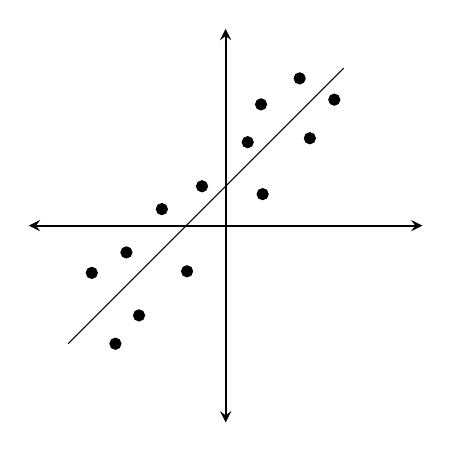
\begin{tikzpicture}
        \draw[black,stealth-stealth, thick] (0,0) -- (5,0);
        \draw[black,stealth-stealth, thick] (2.5,-2.5) -- (2.5,2.5);
        \draw (0.5,-1.5) -- (4,2);
        \filldraw (1.4,-1.14) circle (2pt);
        \filldraw (0.8,-0.6) circle (2pt);
        \filldraw (1.1,-1.5) circle (2pt);
        \filldraw (2.01,-0.58) circle (2pt);
        \filldraw (1.69,0.21) circle (2pt);
        \filldraw (1.24,-0.34) circle (2pt);
        \filldraw (2.97,0.4) circle (2pt);
        \filldraw (2.78,1.06) circle (2pt);
        \filldraw (2.2,0.5) circle (2pt);
        \filldraw (3.57,1.11) circle (2pt);
        \filldraw (2.95,1.54) circle (2pt);
        \filldraw (3.44,1.87) circle (2pt);
        \filldraw (3.88,1.6) circle (2pt);
    \end{tikzpicture}
    \mbox{\textbf{i.} Recta}
\end{center}
~\vspace{-0.5cm}
\begin{center}
    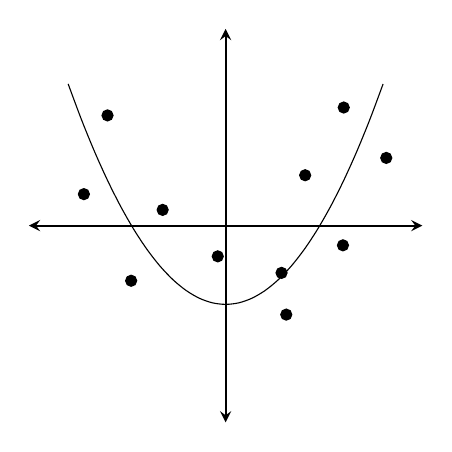
\begin{tikzpicture}
        \draw[black,stealth-stealth, thick] (-2.5,0) -- (2.5,0);
        \draw[black,stealth-stealth, thick] (0,-2.5) -- (0,2.5);
        \draw[domain=-2:2, smooth, variable=\x] plot ({\x}, {0.7*\x*\x-1});
        \filldraw (-1.8,0.4) circle (2pt);
        \filldraw (-0.8,0.2) circle (2pt);
        \filldraw (-1.2,-0.7) circle (2pt);
        \filldraw (-0.1,-0.39) circle (2pt);
        \filldraw (0.77,-1.13) circle (2pt);
        \filldraw (0.71,-0.6) circle (2pt);
        \filldraw (1.49,-0.25) circle (2pt);
        \filldraw (1.01,0.64) circle (2pt);
        \filldraw (2.04,0.86) circle (2pt);
        \filldraw (1.5,1.5) circle (2pt);
        \filldraw (-1.5,1.4) circle (2pt);
    \end{tikzpicture}
    \textbf{ii.} Cuadrática
\end{center}
~\vspace{-0.5cm}
\begin{center}
    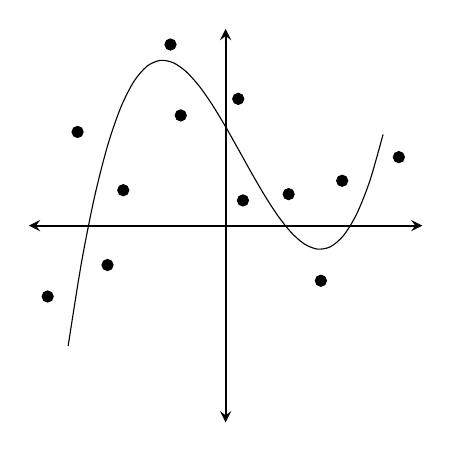
\begin{tikzpicture}
        \draw[black,stealth-stealth, thick] (-2.5,0) -- (2.5,0);
        \draw[black,stealth-stealth, thick] (0,-2.5) -- (0,2.5);
        \draw[domain=-2:2, smooth, variable=\x] plot ({\x}, {0.6*((\x-1.2)^3+3*(\x-1.2)^2-0.5)});
        \filldraw (-1.5,-0.5) circle (2pt);
        \filldraw (-2.26,-0.9) circle (2pt);
        \filldraw (-1.3,0.45) circle (2pt);
        \filldraw (-1.88,1.19) circle (2pt);
        \filldraw (-0.7,2.3) circle (2pt);
        \filldraw (1.21,-0.7) circle (2pt);
        \filldraw (1.48,0.57) circle (2pt);
        \filldraw (2.2,0.87) circle (2pt);
        \filldraw (0.16,1.61) circle (2pt);
        \filldraw (0.22,0.32) circle (2pt);
        \filldraw (0.8,0.4) circle (2pt);
        \filldraw (-0.57,1.4) circle (2pt);
    \end{tikzpicture}
    \textbf{iii.} Cúbica
\end{center}
}

Ya sea en un laboratorio de ingeniería o de física, en un observatorio astronómico o en problemas financieros, relacionados con la estadística o con las ciencias en general, siempre que se tengan una serie de datos que puedan presentarse en forma de parejas ordenadas de números reales, se podrá emplear el método de aproximación por mínimos cuadrados para encontrar una función real de variable real, cuya gráfica sea la curva que mejor ajusta a dichas parejas, es decir, la curva óptima que permite visualizar y predecir la tendencia o comportamiento teórico de los datos. En eso radica la importancia de este método de aproximación.

Muy a menudo los científicos o los economistas tienen que trabajar con grandes cantidades de datos para encontrar relaciones entre las variables de un problema. Una manera común de hacer esto es ajustar una curva entre los distintos puntos de datos. Esta curva puede ser recta o cuadrática o cúbica, y así sucesivamente (en la figura \ref{USUAUJSJSJSKSKKNNSN} se indican tres de las curvas que se pueden utilizar para ajustar datos). El objetivo es encontrar la curva del tipo específico que se ajuste “mejor” a los datos dados.

\subsection*{Aproximación por una recta}

Antes de continuar, debe aclararse qué quiere decir “mejor ajuste”. Suponga que se busca la recta de la forma $y = \tilde{m}x + \tilde{b}$ que mejor represente a los $n$ datos $(x_1, y_1)$, $(x_2, y_2)$, $\dots$, $(x_n, y_n)$. Vea la siguiente figure que ilustra lo que ocurre.
\begin{center}
    \begin{tikzpicture}
        \draw[-stealth,thick] (0,-1) -- (0,6) node[below left] {$y$};
        \draw[-stealth,thick] (-1,0) -- (10,0) node[below left] {$x$};
        \node[below left] at (0,0) {$0$};
        \filldraw (1,1) circle (2pt);
        \filldraw (2,3) circle (2pt);
        \filldraw (3,1.5) circle (2pt);
        \filldraw (5,5) circle (2pt) node[below right] {$(x_i, y_i)$};
        \filldraw (5,3.28) circle (2pt) node[below right] {$\left(x_i, \tilde{m}x_i + \tilde{b}\right)$};
        \filldraw (7,4) circle (2pt);
        \filldraw (8,5) circle (2pt);
        \draw (-1,-0.14) -- (9.75,6);
        \foreach \x in {1,2,3} \draw (\x,0.1) -- (\x,-0.1) node[below] {$x_{\x}$};
        \node[below] at (4,-0.1) {$\cdots$};
        \draw (5,0.1) -- (5,-0.1) node[below] {$x_i$};
        \node[below] at (6,-0.1) {$\cdots$};
        \draw (7,0.1) -- (7,-0.1) node[below] {$x_{n-1}$};
        \draw (8,0.1) -- (8,-0.1) node[below] {$x_n$};
        \draw[decorate,decoration={brace, amplitude=5pt, mirror,raise=1ex}] (5,5) -- (5,3.28) node[midway, xshift=-1.6cm]{$y_i - \left(\tilde{m}x_i + \tilde{b}\right)$};
    \end{tikzpicture}
\end{center}
En esta figura se ve que si se supone que las variables $x$ e $y$ están relacionadas por la fórmula $y = \tilde{m}x + \tilde{b}$, entonces, por ejemplo, para $x = x_1$ el valor correspondiente de $y$ es $\tilde{m}x_1 + \tilde{b}$ (esto es diferente del valor “real”, $y = y_1$). Es decir, la ecuación de la recta queda determinada totalmente por los valores de $\tilde{m}$ y $\tilde{b}$.

Por lo tanto, al determinar la manera de elegir la recta $y = \tilde{m}x + b$ que mejor se aproxima a los datos dados, es razonable usar el criterio de seleccionar aquella que minimiza la suma de los cuadrados de las diferencias entre los valores $y$ de los puntos y el valor $y$ correspondiente a la recta. Observe que la distancia entre $(x_i, y_i)$ y $\left(x_i, \tilde{m}x_i + \tilde{b}\right)$ es $y_i - \left(\tilde{m}x_i + \tilde{b}\right)$, así el problema radica en encontrar los valores de $\tilde{m}$ y $\tilde{b}$ tales que la suma
$$\left[ y_1 - \left(\tilde{m}x_1 + \tilde{b} \right) \right]^2 + \left[ y_2 - \left(\tilde{m}x_2 + \tilde{b} \right) \right]^2 + \cdots + \left[ y_n - \left(\tilde{m}x_n + \tilde{b} \right) \right]^2$$\newpage\noindent
sea mínima. En otras palabras, se desea encontrar
\begin{equation}
    \min_{i} \left\{ \sum_{i=1}^{n} \left[ y_i - \left(\tilde{m}x_i + \tilde{b} \right) \right]^2 \right\} \label{minimoscuadrados1}
\end{equation}
Para estos valores de $\tilde{m}$ y $\tilde{b}$, la recta $y = \tilde{m}x + \tilde{b}$ se llama aproximación por la recta de mínimos cuadrados a los datos $(x_1, y_1)$, $(x_2, y_2)$, $\dots$, $(x_n, y_n)$.

Una vez definido el problema se busca un método para encontrar la aproximación de mínimos cuadrados. Lo más sencillo es escribir todo en forma matricial. De la expresión \eqref{minimoscuadrados1}, se tiene
\begin{align*}
    y_1 & - \left(\tilde{m}x_1 + \tilde{b} \right) \\
    y_2 & - \left(\tilde{m}x_2 + \tilde{b} \right) \\
    & \phantom{-} \vdots \\
    y_n & - \left(\tilde{m}x_n + \tilde{b} \right)
\end{align*}
Entonces,
$$\begin{bmatrix}
    y_1 \\
    y_2 \\
    \vdots \\
    y_n
\end{bmatrix} - \begin{bmatrix}
    1 & x_1 \\
    1 & x_2 \\
    \vdots & \vdots \\
    1 & x_n
\end{bmatrix} \begin{bmatrix}
    \tilde{b} \\
    \tilde{m}
\end{bmatrix} = \mathbb{y} - A \tilde{\mathbb{u}}$$
siendo
$$\mathbb{y} = \begin{bmatrix}
    y_1 \\
    y_2 \\
    \vdots \\
    y_n
\end{bmatrix}, \quad A = \begin{bmatrix}
    1 & x_1 \\
    1 & x_2 \\
    \vdots & \vdots \\
    1 & x_n
\end{bmatrix}, \quad \tilde{\mathbb{u}} = \begin{bmatrix}
    \tilde{b} \\
    \tilde{m}
\end{bmatrix}$$
De lo expuesto anterior, se deduce que
\begin{equation}
    \min_{i} \left\{ \sum_{i=1}^{n} \left[ y_i - \left(\tilde{m}x_i + \tilde{b} \right) \right]^2 \right\} = \min_{i} \left\{ (\mathbb{y} - A \tilde{\mathbb{u}}) \bullet (\mathbb{y} - A \tilde{\mathbb{u}}) \right\} \label{minimoscuadrados2}
\end{equation}
Encontrar el vector $\mathbb{u}$ que minimiza no es tan difícil como parece. Como $A$ es una matriz de $n \times 2$ y $\tilde{\mathbb{u}}$ es una matriz de $2 \times 1$, el vector $A\tilde{\mathbb{u}}$ es un vector en $\RR[n]$ que pertenece a la imagen de $A$. La imagen de $A$ es un subespacio de $\RR[n]$ cuya dimensión es a lo más dos (ya que cuando mucho dos columnas de $A$ son linealmente independientes). En $\RR[3]$ la imagen de $A$ será un plano o una recta que pasa por el origen (ya que estos son los únicos subespacios de $\RR[3]$ de dimensión uno o dos). De manera geométrica en $\RR[3]$, si $H$ es la imagen de $A$, entonces
\begin{center}
    \begin{tikzpicture}
        \begin{axis}[view={35}{25},
            width=11cm,height=11cm,
            xtick=\empty,
            ytick=\empty,
            ztick=\empty,
            xmin=-5, xmax=16,
            ymin=-5, ymax=15,
            zmin=-6, zmax=10,
            axis lines=center,
            %xticklabel=\empty,
            %yticklabel=\empty,
            %zticklabel=\empty,
            axis line style={draw=none},
            ticks=none,
            ]
            \fill[black,opacity=0.1] (xyz cs:x=-5,y=-5,z=0) -- (xyz cs:x=15,y=-5,z=0) -- (xyz cs:x=15,y=15,z=0) -- (xyz cs:x=-5,y=15,z=0) -- cycle;
            \draw[-latex] (0,0,0) -- (4,4,0) node[below left,yshift=-0.1cm] {$\proy_{H} \mathbb{y}$};
            %\draw (4,4,0) -- (4,4,4) node[midway,right,font=\footnotesize] {$\mathbb{y} - \proy_{H} \mathbb{y}$};
            \draw[-latex] (0,0,0) -- (8,8,0) node[below left] {$A\tilde{\mathbb{u}}$};
            \draw[-latex] (0,0,0) -- (8,8,8) node[left]{$\mathbb{y}$};
            \draw[-latex] (8,8,0) -- (8,8,8);
            \node[right] at (8,8,4) {$\mathbb{y} - A\tilde{\mathbb{u}}$};
            \begin{scope}[canvas is xy plane at z=0.5]
                \node at (14,4) [scale=5,transform shape,rotate=90] {Imagen de $A$};
            \end{scope}
        \end{axis}
    \end{tikzpicture}
\end{center}\newpage
De esta manera, del gráfico precedente y de la ecuación \eqref{minimoscuadrados2}, se deduce que $(\mathbb{y} - A \tilde{\mathbb{u}}) \bullet (\mathbb{y} - A \tilde{\mathbb{u}})$ es mínimo cuando $y - A\tilde{\mathbb{u}}$ es ortogonal a la imagen de $A$. En otras palabras, si $\tilde{\mathbb{u}}$ es el vector que minimiza, entonces para cualquier vector $\tilde{\mathbb{u}} \in \RR[2]$ se cumple que
$$(\mathbb{y} - A \tilde{\mathbb{u}}) \perp A\tilde{\mathbb{u}}$$
Según la definición \ref{def:vectoresortogonales}, esto implica que
$$(A\tilde{\mathbb{u}}) \bullet (\mathbb{y} - A\tilde{\mathbb{u}}) = 0$$
es decir,
$$\tilde{\mathbb{u}} \bullet \big( A^T (\mathbb{y} - A\tilde{\mathbb{u}}) \big) = 0$$
lo cual se traduce en
$$\tilde{\mathbb{u}} \bullet \left( A^T\mathbb{y} - A^TA\tilde{\mathbb{u}} \right) = 0$$
y, por ende,
$$A^T\mathbb{y} - A^TA\tilde{\mathbb{u}} = 0$$
De esta igualdad se deduce que
\begin{equation}
    A^T\mathbb{y} = A^TA\tilde{\mathbb{u}} \label{OPAOPAOPAIPAIPA}
\end{equation}
Se desea despejar a $\tilde{\mathbb{u}}$, para ello, se demostrara que si
$$A = \begin{bmatrix}
    1 & x_1 \\
    1 & x_2 \\
    \vdots & \vdots \\
    1 & x_n
\end{bmatrix}$$
y no todos los $x_i$ son iguales, entonces $A^TA$ es una matriz invertible. Así
\begin{align*}
    A^TA & = \begin{bmatrix}
        1 & 1 & \cdots & 1 \\
        x_1 & x_2 & \cdots & x_n
    \end{bmatrix} \begin{bmatrix}
        1 & x_1 \\
        1 & x_2 \\
        \vdots & \vdots \\
        1 & x_n
    \end{bmatrix} \\
    & = \begin{bmatrix}
        n & \displaystyle\sum_{i=1}^{n} x_i \\
        \displaystyle\sum_{i=1}^{n} x_i & \displaystyle\sum_{i=1}^{n}x_i^2
    \end{bmatrix}
\end{align*}
Para probar que $A^TA$ es invertible, bastará probar que $\Det \left(A^T A \right) \neq 0$, donde
$$\Det \left(A^T A\right) = n \sum_{i=1}^{n} x_i^2 - \left( \sum_{i=1}^{n} x_i \right)^2$$
Sean $\mathbb{p}$, $\mathbb{q} \in \RR[n]$ con $ \mathbb{p} = \begin{pmatrix} x_1 \\ x_2 \\ \vdots \\ x_n \end{pmatrix}$ y $\mathbb{q} = \begin{pmatrix} 1 \\ 1 \\ \vdots \\ 1 \end{pmatrix}$, entonces
$$\| \mathbb{p} \|^2 = \sum_{i=1}^{n} x_i^2, \!\quad \| \mathbb{q} \|^2 = n, \quad \text{y} \quad\, \mathbb{p} \bullet \mathbb{q} = \sum_{i=1}^{n} x_i$$
Por tanto, de acuerdo con el teorema \ref{theo:Cauchy-Schwarz}, se sigue que
$$\left( \sum_{i=1}^{n} x_i \right)^2 = (\mathbb{p} \bullet \mathbb{q})^2 \leq \| \mathbb{p} \|^2 \| \mathbb{q} \|^2 = n \sum_{i=1}^{n} x_i^2$$\newpage\noindent
Como no todos los $x_i$ son iguales, entonces $\mathbb{p}$ y $\mathbb{q}$ son linealmente independientes, por tanto
$$(\mathbb{p} \bullet \mathbb{q})^2 < \| \mathbb{p} \|^2 \| \mathbb{q} \|^2$$
En consecuencia,
$$n \sum_{i=1}^{n} x_i^2 - \left( \sum_{i=1}^{n} x_i \right)^2 \neq 0$$
Es decir, $\Det \left(A^T A\right) \neq 0$, y por lo tanto $A^TA$ es invertible. Siguiendo con el objetivo de encontrar a $\tilde{\mathbb{u}}$, de la ecuación \eqref{OPAOPAOPAIPAIPA} se sigue que
$$\begin{bmatrix}
    1 & 1 & \cdots & 1 \\
    x_1 & x_2 & \cdots & x_n
\end{bmatrix} \begin{bmatrix}
    y_1 \\
    y_2 \\
    \vdots \\
    y_n
\end{bmatrix} = \begin{bmatrix}
    1 & 1 & \cdots & 1 \\
    x_1 & x_2 & \cdots & x_n
\end{bmatrix} \begin{bmatrix}
    1 & x_1 \\
    1 & x_2 \\
    \vdots & \vdots \\
    1 & x_n
\end{bmatrix} \begin{bmatrix}
    \tilde{b} \\
    \tilde{m}
\end{bmatrix}$$
es decir,
$$\begin{bmatrix}
    \displaystyle\sum_{i=1}^{n} y_i \\
    \displaystyle\sum_{i=1}^{n} x_iy_i
\end{bmatrix} = \begin{bmatrix}
    n & \displaystyle\sum_{i=1}^{n} x_i \\
    \displaystyle\sum_{i=1}^{n} x_i & \displaystyle\sum_{i=1}^{n}x_i^2
\end{bmatrix} \begin{bmatrix}
    \tilde{b} \\
    \tilde{m}
\end{bmatrix}$$
o equivalentemente
$$\begin{bmatrix}
    \displaystyle n\tilde{b} + \tilde{m} \sum_{i=1}^{n} x_i \\
    \displaystyle\tilde{b} \sum_{i=1}^{n} x_i + \tilde{m} \sum_{i=1}^{n} x_i^2
\end{bmatrix} = \begin{bmatrix}
    \displaystyle\sum_{i=1}^{n} y_i \\
    \displaystyle\sum_{i=1}^{n} x_iy_i
\end{bmatrix}$$
Empleando la regla de Cramer, se sigue que
$$\tilde{b} = \frac{\displaystyle\left( \sum_{i=1}^{n} y_i \right) \left( \sum_{i=1}^{n} x_i^2 \right) - \left( \sum_{i=1}^{n} x_i \right) \left( \sum_{i=1}^{n} x_iy_i \right)}{\displaystyle n \sum_{i=1}^{n} x_i^2 - \left( \sum_{i=1}^{n} x_i \right)^2}$$
y
$$\tilde{m} = \frac{\displaystyle n \sum_{i=1}^{n} x_iy_i - \left( \sum_{i=1}^{n} x_i \right) \left( \sum_{i=1}^{n} x_iy_i \right)}{\displaystyle n \sum_{i=1}^{n} x_i^2 - \left( \sum_{i=1}^{n} x_i \right)^2}$$
o, sin aplicar la regla de Cramer, de la ecuación \eqref{OPAOPAOPAIPAIPA} se puede obtener a $\tilde{m}$ y $\tilde{b}$ con
$$\tilde{\mathbb{u}} = \begin{bmatrix}
    \tilde{b} \\
    \tilde{m}
\end{bmatrix} = \left( A^T A \right)^{-1} A^T \mathbb{y}$$

\begin{example}
    Encontrar la ecuación de la recta que mejor se ajusta para los datos $(1, 4)$, $(-2, 5)$, $(3, -1)$, $(4, 1)$. \\
    \solucion Observemos que
    $$A = \begin{bmatrix*}[r]
        1 & 1 \\
        1 & -2 \\
        1 & 3 \\
        1 & 4
    \end{bmatrix*}, \!\quad A^T = \begin{bmatrix*}[r]
        1 & 1 & 1 & 1 \\
        1 & -2 & 3 & 4
    \end{bmatrix*} \quad \text{y} \quad \mathbb{y} = \begin{bmatrix*}[r]
        4 \\
        5 \\
        -1 \\
        1
    \end{bmatrix*}$$
    entonces
    $$A^TA = \begin{bmatrix}
        4 & 6 \\
        6 & 30
    \end{bmatrix} \quad \text{y} \quad \left(A^T A\right)^{-1} = \frac{1}{84} \begin{bmatrix*}[r]
        30 & -6 \\
        -6 & 4
    \end{bmatrix*}$$\newpage\noindent
    Por lo que\sideFigure[\label{ejemplo_minimoscuadrados}]{
    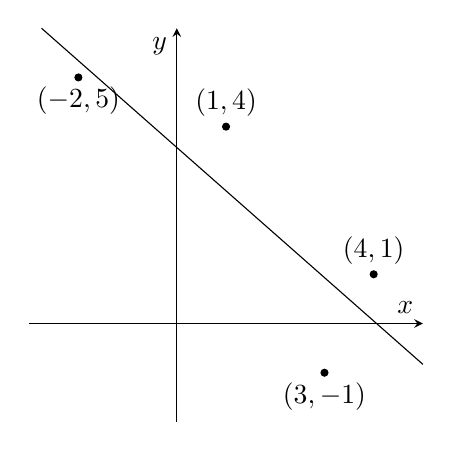
\begin{tikzpicture}[scale=0.625]
        \draw[-stealth] (-3,0) -- (5,0) node[above left] {$x$};
        \draw[-stealth] (0,-2) -- (0,6) node[below left] {$y$};
        \filldraw (-2,5) circle (2pt) node[below] {$(-2, 5)$};
        \filldraw (1,4) circle (2pt) node[above] {$(1, 4)$};
        \filldraw (4,1) circle (2pt) node[above] {$(4, 1)$};
        \filldraw (3,-1) circle (2pt) node[below] {$(3, -1)$};
        \draw (-2.75,6) -- (5,-0.83);
    \end{tikzpicture}
    }
    \begin{align*}
        \tilde{u} & = \frac{1}{84} \begin{bmatrix*}[r]
            30 & -6 \\
            -6 & 4
        \end{bmatrix*} \begin{bmatrix*}[r]
            1 & 1 & 1 & 1 \\
            1 & -2 & 3 & 4
        \end{bmatrix*} \begin{bmatrix*}[r]
            4 \\
            5 \\
            -1 \\
            1
        \end{bmatrix*} \\
        & = \frac{1}{84} \begin{bmatrix*}[r]
            30 & -6 \\
            -6 & 4
        \end{bmatrix*} \begin{bmatrix*}[r]
            9 \\
            -5
        \end{bmatrix*} \\
        & = \frac{1}{84} \begin{bmatrix*}[r]
            300 \\
            -74
        \end{bmatrix*}
    \end{align*}
    Por lo tanto, la recta que mejor se ajusta a los cuatro datos está dada por
    $$y = - \frac{37}{42} x + \frac{25}{7}$$
    Esta recta y los cuatros datos se bosquejan en la figura \ref{ejemplo_minimoscuadrados}.
\end{example}

\subsection*{Aproximación cuadrática}

Ahora se desea ajustar una curva cuadrática a los $n$ datos. Recordemos que una curva cuadrática en $x$ es cualquier expresión de la forma
$$y = a + bx + cx^2$$
Observemos que la ecuación anterior es la ecuación de una parábola en el plano. Si los $n$ datos estuvieran sobre la parábola, se tendría
\begin{align*}
    y_1 & - \left( a + bx_1 + cx_1^2 \right) \\
    y_2 & - \left( a + bx_2 + cx_2^2 \right) \\
    & \phantom{-} \vdots \\
    y_n & - \left( a + bx_n + cx_n^2 \right)
\end{align*}
Entonces,
$$\begin{bmatrix}
    y_1 \\
    y_2 \\
    \vdots \\
    y_n
\end{bmatrix} - \begin{bmatrix}
    1 & x_1 & x_1^2 \\
    1 & x_2 & x_2^2 \\
    \vdots & \vdots & \vdots \\
    1 & x_n & x_n^2
\end{bmatrix} \begin{bmatrix}
    a \\
    b \\
    c
\end{bmatrix} = \mathbb{y} - A \tilde{\mathbb{u}}$$
siendo
$$\mathbb{y} = \begin{bmatrix}
    y_1 \\
    y_2 \\
    \vdots \\
    y_n
\end{bmatrix}, \quad A = \begin{bmatrix}
    1 & x_1 & x_1^2 \\
    1 & x_2 & x_2^2 \\
    \vdots & \vdots & \vdots \\
    1 & x_n & x_n^2
\end{bmatrix}, \quad \tilde{\mathbb{u}} = \begin{bmatrix}
    a \\
    b \\
    c
\end{bmatrix}$$
al igual que antes. Utilizando un razonamiento similar al anterior, se puede demostrar que si cuando menos tres de las $x_i$ son diferentes, entonces $A^TA$ es invertible y el vector que minimiza al vector $\tilde{u}$ está dado por
$$\tilde{\mathbb{u}} = \begin{bmatrix}
    a \\
    b \\
    c
\end{bmatrix} = \left( A^T A \right)^{-1} A^T \mathbb{y}$$

\subsection*{Aproximación polinomial}

El polinomio de grado $k$ está dado por
$$a_0 + a_1 x + a_2 x^2 + \cdots + a_k x^k$$\newpage\noindent
A continuación, demostraremos que el polinomio de grado $k$ que mejor se ajusta a los $n$ puntos está dado por 
$$\tilde{\mathbb{u}} = \begin{bmatrix} a_0 \\ a_1 \\ \vdots \\ a_n \end{bmatrix} = \left( A^T A \right)^{-1} A^T \mathbb{y}$$
donde
$$A = \begin{bmatrix}
1 & x_1 & x_1^2 & \cdots & x_1^k \\
1 & x_2 & x_2^2 & \cdots & x_2^k \\
\vdots & \vdots & \vdots & & \vdots \\
1 & x_n & x_n^2 & \cdots & x_n^k
\end{bmatrix}$$
Para demostrar que el polinomio de grado $k$ que mejor se ajusta a los $n$ puntos está dado por la expresión dada, primero debemos saber que el objetivo es encontrar los coeficientes $a_0, a_1, \dots, a_k$ que minimizan la expresión:
$$\sum_{i=1}^{n} \left[y_i - \left(a_0 + a_1 x_i + a_2 x_i^2 + \cdots + a_k x_i^k\right)\right]^2$$
Esta expresión puede ser escrita de manera matricial como:
$$\| \mathbb{y} - A\tilde{\mathbb{u}} \|^2$$
Donde \( \mathbb{y} \) es el vector columna de los valores observados, \( A \) es la matriz como se definió al principio, y \( \tilde{\mathbb{u}} \) es el vector columna de los coeficientes del polinomio.

Para encontrar los coeficientes que minimizan esta expresión, tomamos la derivada respecto a \( \tilde{\mathbb{u}} \) y la igualamos a cero:
$$\frac{\partial}{\partial \tilde{\mathbb{u}}} \| \mathbb{y} - A\tilde{\mathbb{u}} \|^2 = 0$$
Esto nos lleva a la ecuación normal:
$$A^T \left(A\tilde{\mathbb{u}} - \mathbb{y}\right) = 0$$
Resolviendo para \( \overline{\mathbb{u}} \):
$$A^T A\overline{\mathbb{u}} = A^T \mathbb{y}$$
Y finalmente:
$$\tilde{\mathbb{u}} = \left(A^T A\right)^{-1} A^T \mathbb{y}$$
Esta es la solución que minimiza la suma de los cuadrados de las diferencias y, por lo tanto, da el mejor ajuste polinomial de grado $k$ a los $n$ puntos dados.

\section{Espacios vectoriales con producto interno y proyecciones}

Después de haber establecido una comprensión sólida del producto punto en el espacio $\RR[n]$, es hora de expandir nuestro enfoque hacia la generalización de este concepto a través de los espacios con producto interno. Mientras que el producto punto se limita al espacio euclidiano \(n\)-dimensional, los espacios con producto interno nos permiten extender esta noción a dimensiones superiores y a estructuras más abstractas. Esta generalización nos abrirá las puertas a un mundo de aplicaciones más amplio y nos permitirá explorar propiedades y teoremas más profundos en el álgebra lineal.

\newpage

\begin{definition}\label{def:espaciocomplejo_productointerno}
    Un espacio vectorial complejo $V$ se denomina espacio con producto interno si para cada par ordenado de vectores $\mathbb{u}$ y $\mathbb{v}$ en $V$ existe un número complejo único $\langle \mathbb{u}, \mathbb{v} \rangle$, denominado producto interno de $\mathbb{u}$ y $\mathbb{v}$, tal que si $\mathbb{u}$, $\mathbb{v}$ y $\mathbb{w}$ están en $V$ y $\alpha \in \CC$, entonces\infoBulle{En la definición \ref{def:espaciocomplejo_productointerno}, se está introduciendo la definición de un espacio vectorial complejo con producto interno, sin embargo, aún no hemos explorado detalladamente los espacios vectoriales complejos en sí mismos. Este tema será abordado en el capítulo \ref{chap:espacios_complejos} de esta obra, donde analizaremos las propiedades, operaciones y aplicaciones de estos espacios, proporcionando una comprensión sólida de su papel en el ámbito del álgebra lineal.}
    \begin{enumerate}[label=\roman*)]
        \item $\langle \mathbb{u}, \mathbb{u} \rangle \geq 0$.
        \item $\langle \mathbb{u}, \mathbb{u} \rangle = 0$ si y solo si $\mathbb{u} = \mathbb{0}$.
        \item $\langle \mathbb{u}, \mathbb{v} + \mathbb{w} \rangle = \langle \mathbb{u}, \mathbb{v} \rangle + \langle \mathbb{u}, \mathbb{w} \rangle$.
        \item $\langle \mathbb{u} + \mathbb{v}, \mathbb{w} \rangle = \langle \mathbb{u}, \mathbb{w} \rangle + \langle \mathbb{v}, \mathbb{w} \rangle$.
        \item $\langle \mathbb{u}, \mathbb{v} \rangle = \overline{\langle \mathbb{v}, \mathbb{u} \rangle}$.
        \item $\langle \alpha \mathbb{u}, \mathbb{v} \rangle = \alpha \langle \mathbb{u}, \mathbb{v} \rangle$.
        \item $\langle \mathbb{u}, \alpha \mathbb{v} \rangle = \overline{\alpha} \langle \mathbb{u}, \mathbb{v} \rangle$.
    \end{enumerate}
\end{definition}

\begin{observation}
    Si $\langle \mathbb{u}, \mathbb{v} \rangle$ es real, entonces $\langle \mathbb{u}, \mathbb{v} \rangle = \langle \mathbb{v}, \mathbb{u} \rangle$.
\end{observation}

\begin{observation}
    Se ha optado por adoptar una nueva convención en cuanto a la notación de vectores en $\CC[n]$. En lugar de utilizar la tradicional notación vertical para representar vectores, se ha decidido emplear la notación horizontal. Es decir, en vez de usar
    $$\CC[n] = \left\{ \begin{pmatrix} z_1 \\ z_2 \\ \vdots \\ z_n \end{pmatrix} \mid z_i \in \CC, \text{ para } i = 1, 2, \dots, n \right\}$$
    se usará
    $$\CC[n] = \left\{ (z_1, z_2, \dots, z_n) \mid z_i \in \CC, \text{ para } i = 1, 2, \dots, n \right\}$$
\end{observation}

\begin{example}\label{interno-usual_complejo}
    Sean $\mathbb{x} = (x_1, x_2, \dots, x_n)$ y $\mathbb{y} = (y_1, y_2, \dots, y_n)$ en $\CC[n]$ (recuerde que esto significa que los elementos $x_i$ y $y_i$ son números complejos). Entonces se define\remarkBulle{Sean $z$, $w \in \CC$, entonces
    \begin{enumerate}[label=\roman*., itemsep=3pt]
        \item $\overline{\overline{z}} = z$
        \item $\overline{z+w} = \overline{z} + \overline{w}$
        \item $\overline{zw} = \bar{z} \bar{w}$
        \item $\overline{z/w} = \overline{z}/\overline{w}$
        \item $\bar z + z = 2 \operatorname{Re}(z)$
        \item $\bar z - z = -2 i\operatorname{Im}(z)$
        \item $\overline{z} z =|z|^2 $
        \item $\operatorname{Re}(z) \leq |z|$
        \item $\operatorname{Im}(z) \leq |z|$
        \item $z \in \RR \Leftrightarrow \operatorname{Im}(z)=0$
        \item $z \in \RR \Leftrightarrow \overline{z} = z$
    \end{enumerate}
    }
    $$\mathbb{x} * \mathbb{y} = x_1\overline{y_1} + x_2\overline{y_2} + \cdots + x_n\overline{y_n}$$
    Para validar la definición de la ecuación anterior como un producto interno, es preciso considerar ciertos aspectos relevantes acerca de los números complejos. En caso de que el lector no esté familiarizado con tales conceptos, se sugiere remitirse al \hyperref[chap:numeros-complejos]{Apéndice B} para obtener una comprensión más completa. Posteriormente, procederemos a demostrar las siete propiedades que caracterizan un producto interno:
    \begin{enumerate}[label=\roman*)]
        \item Sea $\mathbb{x} = (x_1, x_2, \dots, x_n)$ en $\CC[n]$, entonces
        \begin{align*}
            \mathbb{x} * \mathbb{x} & = x_1\overline{x_1} + x_2\overline{x_2} + \cdots + x_n\overline{x_n} \\
            & = |x_1|^2 + |x_2|^2 + \cdots + |x_n|^2 \geq 0
        \end{align*}
        \item Sea $\mathbb{x} = (x_1, x_2, \dots, x_n)$ en $\CC[n]$, del inciso anterior
        $$0 = \mathbb{x} * \mathbb{x} = \sum_{j=1}^{n} |x_j|^2 \Longleftrightarrow x_j = 0$$
        para $j = 1, 2, \dots, n$. Así, $|x_j|^2 = 0$ y por lo tanto, $\mathbb{x} = \mathbb{0}$.\newpage
        \item Sean $\mathbb{x} = (x_1, x_2, \dots, x_n)$, $\mathbb{y} = (y_1, y_2, \dots, y_n)$ y $\mathbb{w} = (w_1, w_2, \dots, w_n)$ en $\CC[n]$, entonces
        \begin{align*}
            \mathbb{x} * (\mathbb{y} + \mathbb{w}) & = (x_1, x_2, \dots, x_n) * \left[ (y_1, y_2, \dots, y_n) + (w_1, w_2, \dots, w_n) \right] \\
            & = (x_1, x_2, \dots, x_n) * (y_1 + w_1, y_2 + w_2, \dots, y_n + w_n) \\
            & = x_1 \overline{\left(y_1 + w_1\right)} + x_2 \overline{\left(y_2 + w_2\right)} + \cdots + x_n \overline{\left(y_n + w_n\right)} \\
            & = x_1 \left( \overline{y_1} + \overline{w_1} \right) + x_2 \left( \overline{y_2} + \overline{w_2} \right) + \cdots + x_n \left( \overline{y_n} + \overline{w_n} \right) \\
            & = x_1\overline{y_1} + x_1\overline{w_1} + x_2\overline{y_2} + x_2\overline{w_2} + \cdots + x_n\overline{y_n} + x_n\overline{w_n} \\
            & = x_1\overline{y_1} + x_2\overline{y_2} + \cdots + x_n\overline{y_n} + x_1\overline{w_1} + x_2\overline{w_2} + \cdots + x_n\overline{w_n} \\
            & = \mathbb{x} * \mathbb{y} + \mathbb{x} * \mathbb{w}
        \end{align*}
        \item Sean $\mathbb{x} = (x_1, x_2, \dots, x_n)$, $\mathbb{y} = (y_1, y_2, \dots, y_n)$ y $\mathbb{w} = (w_1, w_2, \dots, w_n)$ en $\CC[n]$, entonces
        \begin{align*}
            (\mathbb{x} + \mathbb{y}) * \mathbb{w} & = \left[ (x_1, x_2, \dots, x_n) + (y_1, y_2, \dots, y_n) \right] * (w_1, w_2, \dots, w_n) \\
            & = (x_1 + y_1, x_2 + y_2, \dots, x_n + y_n) * (w_1, w_2, \dots, w_n) \\
            & = (x_1 + y_1) \overline{w_1} + (x_2 + y_2) \overline{w_2} + \cdots + (x_n + y_n) \overline{w_n} \\
            & = x_1\overline{w_1} + y_1\overline{w_1} + x_2\overline{w_2} + y_2\overline{w_2} + \cdots + x_n\overline{w_n} + y_n\overline{w_n} \\
            & = x_1\overline{w_1} + x_2\overline{w_2} + \cdots + x_n\overline{w_n} + y_1\overline{w_1} + y_2\overline{w_2} + \cdots + y_n\overline{w_n} \\
            & = \mathbb{x} * \mathbb{w} + \mathbb{y} * \mathbb{w}
        \end{align*}
        \item Sean $\mathbb{x} = (x_1, x_2, \dots, x_n)$ y $\mathbb{y} = (y_1, y_2, \dots, y_n)$ en $\CC[n]$, entonces
        \begin{align*}
            \mathbb{x} * \mathbb{y} & = (x_1, x_2, \dots, x_n) * (y_1, y_2, \dots, y_n) \\
            & = x_1\overline{y_1} + x_2\overline{y_2} + \cdots + x_n\overline{y_n} \\
            & = \overline{\overline{x_1}} \, \overline{y_1} + \overline{\overline{x_2}} \, \overline{y_2} + \cdots + \overline{\overline{x_n}} \, \overline{y_n} \\
            & = \overline{\overline{x_1}y_1} + \overline{\overline{x_2}y_2} + \cdots + \overline{\overline{x_n}y_n} \\
            & = \overline{\overline{x_1}y_1 + \overline{x_2}y_2 + \cdots + \overline{x_n}y_n} \\
            & = \overline{y_1\overline{x_1} + y_2\overline{x_2} + \cdots + y_n\overline{x_n}} \\
            & = \overline{\mathbb{y} * \mathbb{x}}
        \end{align*}
        \item Sean $\mathbb{x} = (x_1, x_2, \dots, x_n)$, $\mathbb{y} = (y_1, y_2, \dots, y_n)$ en $\CC[n]$ y $\alpha \in \CC$,
        \begin{align*}
            (\alpha \mathbb{x}) * \mathbb{y} & = (\alpha x_1, \alpha x_2, \dots, \alpha x_n) * (y_1, y_2, \dots, y_n) \\
            & = (\alpha x_1)\overline{y_1} + (\alpha x_2)\overline{y_2} + \cdots + (\alpha x_n)\overline{y_n} \\
            & = \alpha (x_1\overline{y_1}) + \alpha (x_2\overline{y_2}) + \cdots + \alpha (x_n\overline{y_n}) \\
            & = \alpha \left( x_1\overline{y_1} + x_2\overline{y_2} + \cdots + x_n\overline{y_n} \right) \\
            & = \alpha (\mathbb{x} * \mathbb{y})
        \end{align*}
        \item Sean $\mathbb{x} = (x_1, x_2, \dots, x_n)$, $\mathbb{y} = (y_1, y_2, \dots, y_n)$ en $\CC[n]$ y $\alpha \in \CC$,
        \begin{align*}
            \mathbb{x} * (\alpha \mathbb{y}) & = (x_1, x_2, \dots, x_n) * (\alpha y_1, \alpha y_2, \dots, \alpha y_n) \\
            & = x_1 \overline{\left( \alpha y_1 \right)} + x_2 \overline{\left( \alpha y_2 \right)} + \cdots + x_n \overline{\left( \alpha y_n \right)} \\
            & = x_1 \left( \overline{\alpha} \, \overline{y_1} \right) + x_2 \left( \overline{\alpha} \, \overline{y_2} \right) + \cdots + x_n \left( \overline{\alpha} \, \overline{y_n} \right) \\
            & = \overline{\alpha} \left( x_1 \overline{y_1} \right) + \overline{\alpha} \left( x_2 \overline{y_2} \right) + \cdots + \overline{\alpha} \left( x_n \overline{y_n} \right) \\
            & = \overline{\alpha} \left( x_1\overline{y_1} + x_2\overline{y_2} + \cdots + x_n\overline{y_n} \right) \\
            & = \overline{\alpha} (\mathbb{x} * \mathbb{y})
        \end{align*}
    \end{enumerate}
    Dado que la operación $*$ cumple con las siete propiedades que caracterizan un producto interno, se deduce que $*$ representa un producto interno en el espacio $\CC[n]$, comúnmente referido como el producto interno usual en $\CC[n]$.
\end{example}

\newpage

\begin{example}\label{interno_funciones}
    Sea $a < b$ y sea $C[a, b]$ el espacio de funciones de valores reales continuas en el intervalo $[a, b]$. Entonces se define
    $$\langle f, g \rangle = \int_a^b f(t) g(t) dt$$
    Debemos observar que en $C[a, b]$ se supone que los escalares son números reales y que las funciones son de valores reales, de manera que no nos preocupamos por los complejos conjugados. Así, para validar la definición de la ecuación anterior como un producto interno, debemos probar que cumple las siete propiedades de un producto interno.
    \begin{enumerate}[label=\roman*)]
        \item Sea $f \in C[a, b]$, entonces
        \begin{align*}
            \langle f, f \rangle & = \int_a^b f(t) f(t) dt \\
            & = \int_a^b f^2(t) dt \geq 0
        \end{align*}
        \item Se deduce del inciso anterior que $\langle f, f \rangle = 0$ si y solo si $f$ es la función nula en el intervalo $[a, b]$.
        \item Sean $f$, $g$, $h \in C[a, b]$, entonces
        \begin{align*}
            \langle f, g + h \rangle & = \int_a^b f(t) [g(t) + h(t)] dt \\
            & = \int_a^b f(t) g(t) + f(t)h(t) dt \\
            & = \int_a^b f(t) g(t) dt + \int_a^b f(t)h(t) dt \\
            & = \langle f, g \rangle + \langle f, h \rangle
        \end{align*}
        \item Sean $f$, $g$, $h \in C[a, b]$, entonces
        \begin{align*}
            \langle f + g, h \rangle & = \int_a^b [f(t) + g(t)] h(t) dt \\
            & = \int_a^b f(t)h(t) + g(t)h(t) dt \\
            & = \int_a^b f(t)h(t) dt + \int_a^b g(t)h(t) dt \\
            & = \langle f, h \rangle + \langle g, h \rangle
        \end{align*}
        \item Sean $f$, $g \in C[a, b]$, entonces
        \begin{align*}
            \overline{\langle g, f \rangle} & = \overline{\int_a^b g(t)f(t) dt} \\
            & = \int_a^b g(t)f(t) dt \\
            & = \int_a^b f(t)g(t) dt \\
            & = \langle f, g \rangle
        \end{align*}
        \item Se deja como ejercicio al lector.
        \item Es análogo al inciso anterior.
    \end{enumerate}
\end{example}

\newpage

\begin{example}
    Sea $A = \llparenthesis a_{i j} \rrparenthesis$ una matriz de $n \times n$ con entradas reales, la traza de $A$, denotada por $\operatorname{Tr}(A)$, es la suma de las componentes de la diagonal de $A$, es decir,
    $$\operatorname{Tr}(A) = a_{11} + a_{22} + \cdots + a_{nn} = \sum_{i=1}^n \llparenthesis a_{ii} \rrparenthesis$$
    En $\mathcal{M}_{n \times n}(\RR)$ definimos
    \begin{equation}
        \langle A, B \rangle = \operatorname{Tr}\left(A B^{T}\right) \label{usual_matrices}
    \end{equation}
    Demostremos que, en efecto, la expresión anterior es un producto interno en $\mathcal{M}_{n \times n}(\RR)$. Para ello, haremos uso de dos propiedades clave: Consideremos $A = \llparenthesis a_{i j} \rrparenthesis$ y $B = \llparenthesis b_{i j} \rrparenthesis$ matrices de $n \times n$ y sea $\alpha$ un número real (aunque también es válido si $\alpha$ es un número complejo, para nuestros propósitos basta que sea real), entonces
    \begin{enumerate}[label=\Roman*)]
        \item $\operatorname{Tr}(A + B) = \operatorname{Tr}(A) + \operatorname{Tr}(B)$.
        \item $\operatorname{Tr}(\alpha A) = \alpha \operatorname{Tr}(A)$.
    \end{enumerate}
    Demostremos primero, que dichas propiedades se cumplen:
    \begin{enumerate}[label=\Roman*)]
        \item Sean $A$, $B \in \mathcal{M}_{n \times n}(\RR)$, entonces
        \begin{align*}
            \operatorname{Tr}(A + B) & = \sum_{i=1}^n \llparenthesis a_{ii} + b_{ii} \rrparenthesis \\
            & = (a_{11} + b_{11}) + (a_{22} + b_{22}) + \cdots + (a_{nn} + b_{nn}) \\
            & = a_{11} + a_{22} + \cdots + a_{nn} + b_{11} + b_{22} + \cdots + b_{nn} \\
            & = \sum_{i=1}^n \llparenthesis a_{ii} \rrparenthesis + \sum_{i=1}^n \llparenthesis b_{ii} \rrparenthesis \\
            & = \operatorname{Tr}(A) + \operatorname{Tr}(B)
        \end{align*}
        \item Sean $A \in \mathcal{M}_{n \times n}(\RR)$ y $\alpha \in \RR$, entonces
        \begin{align*}
            \operatorname{Tr}(\alpha A) & = \sum_{i=1}^n \llparenthesis \alpha a_{ii} \rrparenthesis \\
            & = (\alpha a_{11}) + (\alpha a_{22}) + \cdots + (\alpha a_{nn}) \\
            & = \alpha \left( a_{11} + a_{22} + \cdots + a_{nn} \right) \\
            & = \alpha \sum_{i=1}^n \llparenthesis a_{ii} \rrparenthesis \\
            & = \alpha \operatorname{Tr}(A)
        \end{align*}
    \end{enumerate}
    A continuación, demostraremos que la expresión \eqref{usual_matrices} es un producto interno, utilizando las propiedades mencionadas anteriormente. Antes de proceder, notemos que
    $$\operatorname{Tr}\left(AB^T\right) = \sum_{i=1}^n \sum_{j=1}^n a_{ij} b_{ij}$$
    Esta expresión representa la suma de los productos de los elementos correspondientes de las matrices $A$ y $B^T$ y será fundamental para la demostración.
    \begin{enumerate}[label=\roman*)]
        \item Sea $A \in \mathcal{M}_{n \times n}(\RR)$, entonces por definición
        $$\langle A, A \rangle = \operatorname{Tr}\left(AA^T\right) = \sum_{i=1}^n \sum_{j=1}^n a_{ij}^2$$
        pero los sumandos del lado derecho son no negativos, lo que prueba que $\langle A, A \rangle \geq 0$.\newpage
        \item Si $\operatorname{Tr}\left(AA^T\right) = 0$, entonces $a_{ij}^2 = 0$ para toda $i$ e $j$, por lo que $A = \mathbb{0}$. Recíprocamente, si $A = \mathbb{0}$, entonces $\langle A, A \rangle = 0$.
        \item Sean $A$, $B$, $C \in \mathcal{M}_{n \times n}(\RR)$, entonces
        \begin{align*}
            \langle A, B + C \rangle & = \operatorname{Tr} \left( A(B + C)^T \right) \\
            & = \operatorname{Tr} \left( AB^T + AC^T \right) \\
            & = \operatorname{Tr} \left( AB^T \right) + \operatorname{Tr} \left( AC^T \right) \\
            & = \langle A, B \rangle + \langle A, C \rangle
        \end{align*}
        \item Sean $A$, $B$, $C \in \mathcal{M}_{n \times n}(\RR)$, entonces
        \begin{align*}
            \langle A + B, C \rangle & = \operatorname{Tr} \left( (A + B)C^T \right) \\
            & = \operatorname{Tr} \left( AC^T + BC^T \right) \\
            & = \operatorname{Tr} \left( AC^T \right) + \operatorname{Tr} \left( BC^T \right) \\
            & = \langle A, C \rangle + \langle B, C \rangle
        \end{align*}
        \item Sean $A$, $B \in \mathcal{M}_{n \times n}(\RR)$, entonces
        \begin{align*}
            \langle A, B \rangle & = \operatorname{Tr}\left(AB^T\right) \\
            & = \sum_{i=1}^n \sum_{j=1}^n a_{ij} b_{ij} \\
            & = \sum_{i=1}^n \sum_{j=1}^n b_{ij} a_{ij} \\
            & = \operatorname{Tr}\left(BA^T\right) \\
            & = \langle B, A \rangle
        \end{align*}
        \item Sean $A$, $B \in \mathcal{M}_{n \times n}(\RR)$ y $\alpha \in \RR$, entonces
        \begin{align*}
            \langle \alpha A, B \rangle & = \operatorname{Tr}\left((\alpha A)B^T\right) \\
            & = \sum_{i=1}^n \sum_{j=1}^n (\alpha a_{ij}) b_{ij} \\
            & = \alpha \sum_{i=1}^n \sum_{j=1}^n a_{ij} b_{ij} \\
            & = \alpha \operatorname{Tr}\left(AB^T\right) \\
            & = \alpha \langle A, B \rangle
        \end{align*}
        \item Sean $A$, $B \in \mathcal{M}_{n \times n}(\RR)$ y $\alpha \in \RR$, entonces
        \begin{align*}
            \langle A, \alpha B \rangle & = \operatorname{Tr}\left(A \left(\alpha B^T \right)\right) \\
            & = \sum_{i=1}^n \sum_{j=1}^n a_{ij} (\alpha b_{ij}) \\
            & = \alpha \sum_{i=1}^n \sum_{j=1}^n a_{ij} b_{ij} \\
            & = \alpha \operatorname{Tr}\left(AB^T\right) \\
            & = \alpha \langle A, B \rangle
        \end{align*}
    \end{enumerate}
    Por lo tanto, la expresión \eqref{usual_matrices} constituye un producto interno en $\mathcal{M}_{n \times n}(\RR)$. En particular, este producto interno es conocido como el producto interno de Frobenius.
\end{example}

\newpage

\begin{observation}
    El producto punto en $\RR[n]$ constituye un producto interno en $\RR[n]$, conocido como el producto interno usual en $\RR[n]$.
\end{observation}

En los próximos desarrollos teóricos, se introducirán definiciones y teoremas en los cuales previamente se empleaba el concepto de producto punto, pero que ahora serán expresados en términos del producto interno. Esta generalización permitirá una mayor flexibilidad y aplicabilidad en diversos contextos matemáticos, además de proporcionar una visión más amplia y profunda de las propiedades y resultados previamente establecidos.

\begin{definition}
    Sea $V$ un espacio vectorial con producto interno $\langle \, , \rangle$. Se define la norma del vector $\mathbb{u} \in V$ como\infoBulle{La expresión $\sqrt{\langle \mathbb{u}, \mathbb{u} \rangle}$ tiene sentido ya que $\langle \mathbb{u}, \mathbb{u} \rangle \geq 0$.}
    $$\| \mathbb{u} \| = \sqrt{\langle \mathbb{u}, \mathbb{u} \rangle}$$
\end{definition}

\begin{observation}
    Es importante señalar que en la definición anterior, la raíz cuadrada que se calcula es la raíz real y no la compleja. Esto es crucial para asegurar la interpretación correcta y la consistencia de la norma en el contexto del espacio vectorial con producto interno dado.
\end{observation}

\begin{definition}\label{orto_prodinterno}
    Sea $V$ un espacio vectorial con producto interno $\langle \, , \rangle$. Dados $\mathbb{u}$, $\mathbb{v} \in V$. Decimos que $\mathbb{u}$ es ortogonal a $\mathbb{v}$ o que $\mathbb{v}$ es ortogonal a $\mathbb{u}$, si $\langle \mathbb{u}, \mathbb{v} \rangle = 0$. En este caso, escribiremos $\mathbb{u} \perp \mathbb{v}$.
\end{definition}

\begin{definition}
    Sea $V$ un espacio vectorial con producto interno $\langle \, , \rangle$. Dados $\mathbb{u}_1$, $\mathbb{u}_2$, $\dots$, $\mathbb{u}_n \in V$.
    \begin{enumerate}[label=\roman*)]
        \item Se dice que el conjunto $\left\{ \mathbb{u}_1, \mathbb{u}_2, \dots, \mathbb{u}_n \right\}$ es un conjunto ortogonal de vectores si $\langle \mathbb{u}_i, \mathbb{u}_j \rangle = 0$, $\forall i \neq j$,
        \item Si además, se cumple que $\sqrt{\langle \mathbb{u}_i, \mathbb{u}_i \rangle} = 1$ para $i = 1$, $2$, $\dots$, $n$, entonces diremos que el conjunto $\left\{ \mathbb{u}_1, \mathbb{u}_2, \dots, \mathbb{u}_n \right\}$ es un conjunto ortonormal de vectores.
    \end{enumerate}
\end{definition}

\begin{theorem}
    Cualquier conjunto finito de vectores ortogonales diferentes del vector  cero en un espacio vectorial con producto interno es linealmente independiente. \\
    \demostracion Sea $V$ un espacio vectorial con producto interno $\langle \, , \rangle$. Dados $\mathbb{u}_1$, $\mathbb{u}_2$, $\dots$, $\mathbb{u}_n \in V$ tal que $\left\{ \mathbb{u}_1, \mathbb{u}_2, \dots, \mathbb{u}_n \right\}$ sea un conjunto ortogonal y
    $$\mathbb{0} = \alpha_1\mathbb{u}_1 + \alpha_2\mathbb{u}_2 + \cdots + \alpha_n\mathbb{u}_n$$
    con $\alpha_i \in \CC$, debemos probar que $\alpha_i = 0$ para $i = 1, 2, \dots, n$. Así,
    \begin{align*}
        0 = \langle \mathbb{u}_i, \mathbb{0} \rangle & = \langle \mathbb{u}_i, \alpha_1\mathbb{u}_1 + \alpha_2\mathbb{u}_2 + \cdots + \alpha_n\mathbb{u}_n \rangle \\
        & = \langle \mathbb{u}_i, \alpha_1 \mathbb{u}_1 \rangle + \langle \mathbb{u}_i, \alpha_2 \mathbb{u}_1 \rangle + \cdots + \langle \mathbb{u}_i, \alpha_i \mathbb{u}_i \rangle + \cdots + \langle \mathbb{u}_i, \alpha_n \mathbb{u}_n \rangle \\
        & = \overline{\alpha_1} \langle \mathbb{u}_i, \mathbb{u}_1 \rangle + \overline{\alpha_2} \langle \mathbb{u}_i, \mathbb{u}_2 \rangle + \cdots + \overline{\alpha_i} \langle \mathbb{u}_i, \mathbb{u}_i \rangle + \cdots + \overline{\alpha_n} \langle \mathbb{u}_i, \mathbb{u}_n \rangle \\
        & = \overline{\alpha_1} \cdot 0 + \overline{\alpha_2} \cdot 0 + \cdots + \overline{\alpha_i} \| \mathbb{u}_i \|^2 + \cdots + \overline{\alpha_n} \cdot 0
    \end{align*}
    Dado que $\mathbb{u}_i \neq \mathbb{0}$ por hipótesis, se infiere que $\| \mathbb{u}_i \|^2 > 0$. Consecuentemente, $\overline{\alpha_i} = 0$, de donde se concluye que $\alpha_i = 0$ para toda $i = 1, 2, \dots, n$. Por consiguiente, los vectores $\mathbb{u}_1$, $\mathbb{u}_2$, $\dots$, $\mathbb{u}_n$ son linealmente independientes.
\end{theorem}

\begin{theorem}
    Cualquier conjunto finito linealmente independiente en un espacio con producto interno se puede convertir en un conjunto ortonormal mediante el proceso de Gram-Schmidt. En particular, cualquier espacio con producto interno tiene una base ortonormal.
\end{theorem}

\begin{example}
    Encuentre una base ortonormal para $P_2[-1, 1]$. \\
    \solucion Observemos que podemos utilizar la base estándar $\left\{ 1, x, x^2 \right\}$. \newpage\noindent Además, notemos que podemos utilizar el producto interno definido en el ejemplo \ref{interno_funciones}. Así, aplicando el proceso de ortonormalización de Gram-Schmidt con $\mathbb{v} = 1$, $\mathbb{v}_2 = x$, $\mathbb{v}_3 = x^2$, se sigue que $\mathbb{v}_1 = \mathbb{u}_1$, por lo que
    \begin{align*}
        \hat{\mathbb{u}}_1 & = \frac{1}{\sqrt{\langle \mathbb{v}_1, \mathbb{v}_1 \rangle}} \mathbb{v}_1 \\
        & = \frac{1}{\sqrt{\displaystyle\int_{-1}^{1} (1)(1) dx}} \cdot 1 \\
        & = \frac{1}{\sqrt{2}}
    \end{align*}
    Luego,
    \begin{align*}
        \mathbb{u}_2 & = x - \langle x, \hat{\mathbb{u}}_1 \rangle \hat{\mathbb{u}}_1 \\
        & = x - \left( \int_{-1}^{1} x \cdot \frac{1}{\sqrt{2}} dx \right) \frac{1}{\sqrt{2}} \\
        & = x - \frac{1}{2} \int_{-1}^{1} x dx \\
        & = x
    \end{align*}
    Ahora,
    \begin{align*}
        \hat{\mathbb{u}}_2 & = \frac{1}{\| \mathbb{u}_2 \|} \mathbb{u}_2 \\
        & = \frac{1}{\displaystyle\int_{-1}^{1} (x)(x) dx} \cdot x \\
        & = \frac{\sqrt{3}}{\sqrt{2}} x
    \end{align*}
    Por último,
    \begin{align*}
        \mathbb{u}_3 & = x^2 - \langle x^2, \hat{\mathbb{u}}_3 \rangle \hat{\mathbb{u}}_3 - \langle x^2, \hat{\mathbb{u}}_2 \rangle \hat{\mathbb{u}}_2 \\
        & = x^2 - \left( \int_{-1}^{1} x^2 \cdot \frac{1}{\sqrt{2}} dx \right) \frac{1}{\sqrt{2}} - \left( \int_{-1}^{1} x^2 \cdot \frac{\sqrt{3}}{\sqrt{2}} x dx \right) \frac{\sqrt{3}}{\sqrt{2}} x \\
        & = \frac{1}{3} \left( 3x^2 - 1 \right)
    \end{align*}
    Además,
    \begin{align*}
        \hat{\mathbb{u}}_3 & = \frac{1}{\| \mathbb{u}_3 \|} \mathbb{u}_3 \\
        & = \frac{1}{\displaystyle\int_{-1}^{1} \left[ \frac{1}{3} \left( 3x^2 - 1 \right) \right] \left[ \frac{1}{3} \left( 3x^2 - 1 \right) \right] dx} \cdot \frac{1}{3} \left( 3x^2 - 1 \right) \\
        & = \sqrt{\frac{5}{8}} \left( 3x^2 - 1 \right)
    \end{align*}
    Por lo tanto, $\displaystyle\left\{ \frac{1}{\sqrt{2}}, \sqrt{\frac{3}{2}} x, \sqrt{\frac{5}{8}} \left( 3x^2 - 1 \right) \right\}$ es una base ortonormal de $P_2[-1, 1]$ con el producto interno definido en el ejemplo \ref{interno_funciones}.
\end{example}

\begin{definition}
    Sea $V$ un espacio vectorial de dimensión finita $n$, con producto interno $\langle \, , \rangle$. Sea $H \subseteq V$ un subespacio de dimensión menor o igual a $n$ y sea $\left\{ \hat{\mathbb{u}}_1, \hat{\mathbb{u}}_2, \dots, \hat{\mathbb{u}}_k \right\}$ una base ortonormal de $H$. Dado $\mathbb{v} \in V$, definimos la proyección ortogonal de $\mathbb{v}$ sobre $H$, denotado por $\proy_{H} \mathbb{v}$, como
    $$\proy_{H} \mathbb{v} = \langle \mathbb{v}, \hat{\mathbb{u}}_1 \rangle \hat{\mathbb{u}}_1 + \langle \mathbb{v}, \hat{\mathbb{u}}_2 \rangle \hat{\mathbb{u}}_2 + \cdots + \langle \mathbb{v}, \hat{\mathbb{u}}_k \rangle \hat{\mathbb{u}}_k$$
    Además, la expresión $\langle \mathbb{v}, \hat{\mathbb{u}}_k \rangle \hat{\mathbb{u}}_k$ se leerá: el producto interno entre $\mathbb{v}$ y $\hat{\mathbb{u}}_k$ en la dirección $\hat{\mathbb{u}}_k$.
\end{definition}

\begin{definition}
    Sea $V$ un espacio vectorial con producto interno $\langle \, , \rangle$. Sea $H$ un subespacio de $V$. El complemento ortogonal de $H$, denotado por $H^{\bot}$, se define como
    $$H^{\bot} = \left\{ \mathbb{x} \in V \mid \langle \mathbb{x}, \mathbb{h} \rangle = 0, \text{ para toda } \mathbb{h} \in H \right\}$$
\end{definition}

\begin{theorem}
    Sea $V$ un espacio vectorial de dimensión finita con producto interno $\langle \, , \rangle$. Sea $H$ un subespacio de $V$, entonces
    \begin{enumerate}[label=\roman*)]
        \item $H^{\bot}$ es subespacio de $V$.
        \item $H \cap H^{\bot} = \{ \mathbb{0} \}$.
        \item $\Dim H^{\bot} = n - \Dim H$.
    \end{enumerate}
    \demostracion
    \begin{enumerate}[label=\roman*)]
        \item Para probar que $H^{\bot}$ es subespacio de $V$, debemos probar que $H^{\bot}$ cumple los dos axiomas de cerradura. Sean $\mathbb{x}$, $\mathbb{y} \in H^{\bot}$, entonces
        $$\langle \mathbb{x}, \mathbb{h} \rangle = 0, \text{ para toda } \mathbb{h} \in H$$
        e
        $$\langle \mathbb{y}, \mathbb{h} \rangle = 0, \text{ para toda } \mathbb{h} \in H$$
        Así
        \begin{align*}
            0 & = 0 + 0 \\
            & = \langle \mathbb{x}, \mathbb{h} \rangle + \langle \mathbb{y}, \mathbb{h} \rangle \\
            & = \langle \mathbb{x} + \mathbb{y}, \mathbb{h} \rangle
        \end{align*}
        Por lo tanto, $\mathbb{x} + \mathbb{y} \in H^{\bot}$. De manera análoga, sean $\mathbb{x} \in H^{\bot}$ y $\alpha \in \RR$, entonces
        \begin{align*}
            \langle \alpha \mathbb{x},  \mathbb{h} \rangle & = \alpha \langle \mathbb{x}, \mathbb{h} \rangle \\
            & = \alpha \cdot 0 \\
            & = 0
        \end{align*}
        En consecuencia, $\alpha \mathbb{x} \in H^{\bot}$. Dado que se cumplen ambas propiedades de cerradura, se concluye que $H^{\bot}$ es un subespacio de $V$.
        \item Sea $\mathbb{x} \in H \cap H^{\bot} \Longrightarrow \mathbb{x} \in H$ \& $\mathbb{x} \in H^{\bot} \Longrightarrow \mathbb{x} \in H$ \& $\langle \mathbb{x}, \mathbb{h} \rangle = 0$, para toda $\mathbb{h} \in H$. Específicamente, esto se cumple cuando $\mathbb{h}$ es igual a $\mathbb{x}$, lo que resulta en $\langle \mathbb{x}, \mathbb{x} \rangle = 0$ o, equivalentemente, $\| \mathbb{x} \|^2 = 0$. Se concluye que $\mathbb{x} = \mathbb{0}$. Por lo tanto, $H \cap H^{\bot} = \{ \mathbb{0} \}$.
        \item Sea $H$ un subespacio de $V$ y sea $\left\{ \hat{\mathbb{u}}_1, \hat{\mathbb{u}}_2, \dots, \hat{\mathbb{u}}_n \right\}$ una base ortonormal de $V$, siendo
        $$\langle \hat{\mathbb{u}}_i, \hat{\mathbb{u}}_j \rangle = \begin{cases}
            1 & \text{ si } i = j \\
            0 & \text{ si } i \neq j
        \end{cases} \qquad \text{para } i, j = 1, 2, \dots, n$$
        Dado que $H \subseteq V$, supongamos que $H = \Gen \left( \left\{ \hat{\mathbb{u}}_1, \hat{\mathbb{u}}_2, \dots, \hat{\mathbb{u}}_k \right\} \right)$ con $k \leq n$, así que asumimos que
        $$H^{\bot} = \Gen \left( \left\{ \hat{\mathbb{u}}_{k+1}, \hat{\mathbb{u}}_{k+2}, \dots, \hat{\mathbb{u}}_n \right\} \right)$$
        Así pues, demostremos que, en efecto, es cierto lo anterior. Sea $\mathbb{w}$ un elemento de $H^{\bot}$, entonces
        $$\mathbb{w} = \beta_{k+1} \hat{\mathbb{u}}_{k+1} + \beta_{k+2} \hat{\mathbb{u}}_{k+2} + \cdots + \beta_n \hat{\mathbb{u}}_n$$
        Ahora, sea $\mathbb{h} \in H$, entonces
        $$\mathbb{h} = \alpha_1 \hat{\mathbb{u}}_1 + \alpha_2 \hat{\mathbb{u}}_2 + \cdots + \alpha_k \hat{\mathbb{u}}_n$$
        Así, se sigue que (análogo a la demostración del teorema \ref{tres_teoremas_fuertes})
        $$\langle \mathbb{w}, \mathbb{h} \rangle = 0$$
        Por lo tanto, $H^{\bot} = \Gen \left( \left\{ \hat{\mathbb{u}}_{k+1}, \hat{\mathbb{u}}_{k+2}, \dots, \hat{\mathbb{u}}_n \right\} \right)$ sí es el complemento ortogonal de $H$. De esta forma,
        \begin{align*}
            \Dim H + \Dim H^{\bot} & = k + (n - k) \\
            & = n
        \end{align*}
        Por lo tanto, $\Dim H^{\bot} = n - \Dim H$.
    \end{enumerate}
\end{theorem}

\begin{theorem}
    Sea $V$ un espacio vectorial de dimensión finita $n$ con producto interno $\langle \, , \rangle$. Sea $H$ un subespacio de $V$ y sea $\mathbb{v} \in V$. Entonces existe un par único de vectores $\mathbb{h} \in H$ y $\mathbb{k} \in H^{\bot}$ tales que
    $$\mathbb{v} = \mathbb{h} + \mathbb{k}$$
    Más aún,
    $$\mathbb{v} = \proy_{H}\mathbb{v} + \proy_{H^{\bot}}\mathbb{v}$$
    \demostracion Sea $\left\{ \hat{\mathbb{u}}_1, \hat{\mathbb{u}}_2, \dots, \hat{\mathbb{u}}_n \right\}$ una base ortonormal de $V$. Análogo a la demostración del teorema \ref{suma_proyecciones}, tenemos que
    \begin{align*}
        \mathbb{v} & = \langle \mathbb{v}, \hat{\mathbb{u}}_1 \rangle \hat{\mathbb{u}}_1 + \langle \mathbb{v}, \hat{\mathbb{u}}_2 \rangle \hat{\mathbb{u}}_2 + \cdots + \langle \mathbb{v}, \hat{\mathbb{u}}_n \rangle \hat{\mathbb{u}}_n \\
        & = \langle \mathbb{v}, \hat{\mathbb{u}}_1 \rangle \hat{\mathbb{u}}_1 + \langle \mathbb{v}, \hat{\mathbb{u}}_2 \rangle \hat{\mathbb{u}}_2 + \cdots + \langle \mathbb{v}, \hat{\mathbb{u}}_k \rangle \hat{\mathbb{u}}_k + \langle \mathbb{v}, \hat{\mathbb{u}}_{k+1} \rangle \hat{\mathbb{u}}_{k+1} + \langle \mathbb{v}, \hat{\mathbb{u}}_{k+2} \rangle \hat{\mathbb{u}}_{k+2} + \cdots + \langle \mathbb{v}, \hat{\mathbb{u}}_n \rangle \hat{\mathbb{u}}_n \\
        & = \proy_{H}\mathbb{v} + \proy_{H^{\bot}}\mathbb{v} \\
        & = \mathbb{h} + \mathbb{k}
    \end{align*}
    siendo $\mathbb{h} = \proy_{H}\mathbb{v}$ y $\mathbb{k} = \proy_{H^{\bot}}\mathbb{v}$.
\end{theorem}

\begin{theorem}[Teorema de aproximación de la norma]
    Sea $V$ un espacio vectorial de dimensión finita con producto interno $\langle \, , \rangle$. Sea $H$ un subespacio de $V$ y sea $\mathbb{v}$ un vector en $V$. Entonces $\proy_{H}\mathbb{v}$ es la mejor aproximación para $\mathbb{v}$ en $H$ en el siguiente sentido: si $\mathbb{h}$ es cualquier otro vector en $H$, entonces
    $$\| \mathbb{v} - \proy_{H}\mathbb{v} \| < \| \mathbb{v} - \mathbb{h} \|$$
    \demostracion Del teorema anterior, tenemos que $\mathbb{v} - \proy_{H} \mathbb{v} \in H^{\bot}$. Así, podemos escribir
    $$\mathbb{v} - \mathbb{h} = (\mathbb{v} - \proy_{H}\mathbb{v}) + (\proy_{H}\mathbb{v} - \mathbb{h})$$
    El primer término de la derecha está en $H^{\bot}$, mientras que el segundo está en $H$. De esta forma,
    $$\langle \mathbb{v} - \proy_{H}\mathbb{v}, \proy_{H}\mathbb{v} - \mathbb{h} \rangle = 0$$
    Así pues, se sigue que
    \begin{align*}
        \| \mathbb{v} - \mathbb{h} \|^2 & = \langle \mathbb{v} - \proy_{H}\mathbb{v}, \proy_{H}\mathbb{v} - \mathbb{h} \rangle \\
        & = \langle (\mathbb{v} - \proy_{H}\mathbb{v}) + (\proy_{H}\mathbb{v} - \mathbb{h}), (\mathbb{v} - \proy_{H}\mathbb{v}) + (\proy_{H}\mathbb{v} - \mathbb{h}) \rangle \\
        & = \| \mathbb{v} - \proy_{H}\mathbb{v} \|^2 + 2 \langle \mathbb{v} - \proy_{H}\mathbb{v},  \mathbb{v} - \proy_{H}\mathbb{v} \rangle + \|\proy_{H}\mathbb{v} - \mathbb{h} \|^2 \\
        & = \| \mathbb{v} - \proy_{H}\mathbb{v} \|^2 + \| \proy_{H}\mathbb{v} - \mathbb{h} \|^2
    \end{align*}
    Pero $\| \proy_{H} \mathbb{v} - \mathbb{h} \|^2 > 0$, ya que $\mathbb{h} \neq \proy_{H}\mathbb{v}$. Por lo tanto,
    $$\| \mathbb{v} - \proy_{H}\mathbb{v} \|^2 < \| \mathbb{v} - \mathbb{h} \|^2$$\newpage\noindent
    es decir,
    $$\| \mathbb{v} - \proy_{H}\mathbb{v} \| < \| \mathbb{v} - \mathbb{h} \|$$
\end{theorem}

\begin{theorem}[Desigualdad de Cauchy-Schwarz]
    Sea $V$ un espacio vectorial con producto interno $\langle \, , \rangle$. Sean $\mathbb{x}$, $\mathbb{y} \in V$, entonces se cumple
    $$| \langle \mathbb{x}, \mathbb{y} \rangle | \leq \| \mathbb{x} \| \| \mathbb{y} \|.$$
    \demostracion Sean $\mathbb{x}$, $\mathbb{y} \in V$, con $\mathbb{y} \neq \mathbb{0}$ y sea $\lambda \in \CC$. Consideremos al vector $\mathbb{x} + \lambda \mathbb{y}$, entonces se tiene
    \begin{align*}
        0 \leq \| \mathbb{x} + \lambda \mathbb{y} \|^2 & = \langle \mathbb{x} + \lambda\mathbb{y}, \mathbb{x} + \lambda\mathbb{y} \rangle \\
        & = \langle \mathbb{x}, \mathbb{x} + \lambda \mathbb{y} \rangle + \langle \lambda \mathbb{y}, \mathbb{x} + \lambda\mathbb{y} \rangle \\
        & = \langle \mathbb{x}, \mathbb{x} \rangle + \langle \mathbb{x}, \lambda \mathbb{y} \rangle + \langle \lambda \mathbb{y}, \mathbb{x} \rangle + \langle \lambda \mathbb{y}, \lambda \mathbb{y} \rangle \\
        & = \langle \mathbb{x}, \mathbb{x} \rangle + \overline{\lambda} \langle \mathbb{x}, \mathbb{y} \rangle + \lambda \langle \mathbb{y}, \mathbb{x} \rangle + \lambda \langle \mathbb{y}, \lambda \mathbb{y} \rangle \\
        & = \langle \mathbb{x}, \mathbb{x} \rangle + \overline{\lambda} \langle \mathbb{x}, \mathbb{y} \rangle + \lambda \overline{\langle \mathbb{x}, \mathbb{y} \rangle} + \lambda\overline{\lambda} \langle \mathbb{y}, \mathbb{y} \rangle \\
        & = \| \mathbb{x} \|^2 + \overline{\lambda} \langle \mathbb{x}, \mathbb{y} \rangle + \lambda \overline{\langle \mathbb{x}, \mathbb{y} \rangle} + |\lambda|^2 \| \mathbb{y} \|^2
    \end{align*}
    Así,
    $$0 \leq \| \mathbb{x} + \lambda \mathbb{y} \|^2 = \| \mathbb{x} \|^2 + \overline{\lambda} \langle \mathbb{x}, \mathbb{y} \rangle + \lambda \overline{\langle \mathbb{x}, \mathbb{y} \rangle} + |\lambda|^2 \| \mathbb{y} \|^2$$
    Entonces
    \begin{equation}
        0 \leq \| \mathbb{x} \|^2 + \overline{\lambda} \langle \mathbb{x}, \mathbb{y} \rangle + \lambda \overline{\langle \mathbb{x}, \mathbb{y} \rangle} + |\lambda|^2 \| \mathbb{y} \|^2 \label{desigualdad-cauchy}
    \end{equation}
    lo cual es válido para cualquier $\lambda \in \CC$, en particular para $\displaystyle \lambda = \frac{(-1)\langle \mathbb{x}, \mathbb{y} \rangle}{\| \mathbb{y} \|^2}$. Además, es evidente que $\displaystyle \overline{\lambda} = \frac{(-1)\overline{\langle \mathbb{x}, \mathbb{y} \rangle}}{\| \mathbb{y} \|^2}$. Así que,
    $$|\lambda|^2 = \frac{(-1)\langle \mathbb{x}, \mathbb{y} \rangle}{\| \mathbb{y} \|^2} \cdot \frac{(-1)\overline{\langle \mathbb{x}, \mathbb{y} \rangle}}{\| \mathbb{y} \|^2} = \frac{|\langle \mathbb{x}, \mathbb{y} \rangle|^2}{\| \mathbb{y} \|^4}$$
    Sustituyendo $\lambda$, $\overline{\lambda}$ y $|\lambda|^2$ en la expresión \eqref{desigualdad-cauchy}, se sigue que
    \begin{align*}
        0 & \leq \| \mathbb{x} \|^2 - \frac{\overline{\langle \mathbb{x}, \mathbb{y} \rangle}}{\| \mathbb{y} \|^2} \langle \mathbb{x}, \mathbb{y} \rangle - \frac{\langle \mathbb{x}, \mathbb{y} \rangle}{\| \mathbb{y} \|^2} \overline{\langle \mathbb{x}, \mathbb{y} \rangle} + \frac{|\langle \mathbb{x}, \mathbb{y} \rangle|^2}{\| \mathbb{y} \|^4} \| \mathbb{y} \|^2 \\
        & = \| \mathbb{x} \|^2 - \frac{|\langle \mathbb{x}, \mathbb{y} \rangle|^2}{\| \mathbb{y} \|^2} - \frac{|\langle \mathbb{x}, \mathbb{y} \rangle|^2}{\| \mathbb{y} \|^2} + \frac{|\langle \mathbb{x}, \mathbb{y} \rangle|^2}{\| \mathbb{y} \|^2} \\
        & = \| \mathbb{x} \|^2 - \frac{|\langle \mathbb{x}, \mathbb{y} \rangle|^2}{\| \mathbb{y} \|^2}
    \end{align*}
    Entonces
    $$\frac{|\langle \mathbb{x}, \mathbb{y} \rangle|^2}{\| \mathbb{y} \|^2} \leq \| \mathbb{x} \|^2$$
    de donde se sigue que
    $$|\langle \mathbb{x}, \mathbb{y} \rangle|^2 \leq \| \mathbb{x} \|^2 \| \mathbb{y} \|^2$$
    Así, finalmente obtenemos que
    $$|\langle \mathbb{x}, \mathbb{y} \rangle| \leq \| \mathbb{x} \| \| \mathbb{y} \|$$
\end{theorem}

\begin{observation}
    Si $\mathbb{x}$ e $\mathbb{y}$ son linealmente dependientes, entonces
    $$|\langle \mathbb{x}, \mathbb{y} \rangle| = \| \mathbb{x} \| \| \mathbb{y} \|$$
    Si $\mathbb{x}$ e $\mathbb{y}$ son linealmente independientes, entonces
    $$|\langle \mathbb{x}, \mathbb{y} \rangle| < \| \mathbb{x} \| \| \mathbb{y} \|$$
\end{observation}

\begin{theorem}\label{JAJSJSJSJJSJSHSTTYQUUQHIAIIQVVCGTQYHHAHAHA}
    Sea $V$ un espacio vectorial con producto interno $\langle \, , \rangle$. Sean $A \in \mathcal{M}_{n \times n}(\RR)$, $\mathbb{x} \in V$, y $\mathbb{y} \in V$. Entonces
    $$\langle A\mathbb{x}, \mathbb{y} \rangle = \left\langle \mathbb{x}, A^T\mathbb{y} \right\rangle$$
    \demostracion La demostración se propone como ejercicio al lector.
\end{theorem}

\newpage

\section{Ejercicios}

\noindent De los problemas 1 al 16 construya una base ortonormal para el espacio o subespacio vectorial dado.
\begin{enumerate}
    \item $\begin{pmatrix*}[r]1 \\ -3\end{pmatrix*},\begin{pmatrix*}3 \\ 0\end{pmatrix*}$.
    \item En $\RR[2]$, comenzando con los vectores básicos $\begin{pmatrix*}1 \\ 1\end{pmatrix*},\begin{pmatrix*}[r]-1 \\ 1\end{pmatrix*}$.
    \item $H=\left\{(x, y) \in \RR[2] \mid x+y=0\right\}$.
    \item $H=\left\{(x, y) \in \RR[2] \mid 2 x+y=0\right\}$.
    \item $H=\left\{(x, y) \in \RR[2] \mid a x+b y=0\right\}$.
    \item En $\RR[2]$, comenzando con $\begin{pmatrix*}a \\ b\end{pmatrix*},\begin{pmatrix*}c \\ d\end{pmatrix*}$, donde $a d-b c \neq 0$.
    \item $\pi=\{(x, y, z) \mid 2 x-y-z=0\}$
    \item $H=\left\{(x, y, z) \in \RR[3] \mid 2 x+y=0\right\}$
    \item $\pi=\left\{(x, y, z) \in \RR[3] \mid x+2 y+3 z=0\right\}$
    \item $H=\left\{(x, y, z) \in \RR[3] \mid x=3 t, y=4 t, z=0, \text{ con }t \in \RR\right\}$
    \item $L=\left\{(x, y, z) \in \RR[3] \mid x=t, y=2 t, z=-2 t, \text{ con }t \in \RR\right\}$
    \item $H=\left\{(x, y, z, w) \in \RR[4] \mid 3 x+4 y+2 z+5 w=0\right\}$
    \item $\pi=\{(x, y, z) \mid a x+b y+c z=0\}$, donde $a b c \neq 0$
    \item $H=\left\{\left(x_{1}, x_{2}, x_{3}, x_{4}, x_{5}\right) \in \RR[5] \mid 2 x_{1}-3 x_{2}+x_{3}+4 x_{4}-x_{5}=0\right\}$
    \item $H=\left\{\left(x_{1}, x_{2}, x_{3}, x_{4}, x_{5}\right) \in \RR[5] \mid x_{1}+2 x_{2}-2 x_{3}-x_{4}-x_{5}=0\right\}$
    \item $H$ es el espacio de soluciones de
    \begin{align*}
        x-3 y+z & = 0 \\
        -2 x+2 y-3 z & = 0 \\
        4 x-8 y+5 z & = 0
    \end{align*}
    \item Encuentre una base ortonormal en $\RR[2]$ que incluya al vector $\mathbb{v}=\begin{pmatrix*}5 \\ 2\end{pmatrix*}$.
    \item Encuentre una base ortonormal en $\RR[3]$ que incluya al vector $\mathbb{v}=\begin{pmatrix*}[r]-3 \\ 2 \\ -1\end{pmatrix*}$.
    \item Encuentre una base ortonormal en $\RR[4]$ que incluya los vectores
    $$\mathbb{u}_{1}=\begin{pmatrix*}
        \displaystyle\frac{1}{\sqrt{2}} \\[3mm]
        0 \\
        \displaystyle\frac{1}{\sqrt{2}} \\[3mm]
        0
    \end{pmatrix*} \quad \text{ y } \quad \mathbb{u}_{2}=\begin{pmatrix*}[r]
        \displaystyle-\frac{1}{2} \\[3mm]
        \displaystyle\frac{1}{2} \\[3mm]
        \displaystyle\frac{1}{2} \\[3mm]
        \displaystyle-\frac{1}{2}
    \end{pmatrix*}$$\newpage
    \item Demuestre que $Q=\begin{bmatrix*}[r] \dfrac{2}{3} & \dfrac{1}{3} & \dfrac{2}{3} \\[2mm] \dfrac{1}{3} & \dfrac{2}{3} & -\dfrac{2}{3} \\[2mm] -\dfrac{2}{3} & \dfrac{2}{3} & \dfrac{1}{3} \end{bmatrix*}$ es una matriz ortogonal.
    \item Demuestre que si $P$ y $Q$ son matrices ortogonales de $n \times n$, entonces $P Q$ es ortogonal.
    \item Verifique el resultado del problema anterior con
    $$P=\begin{bmatrix*}[r]
        \dfrac{1}{\sqrt{2}} & -\dfrac{1}{\sqrt{2}} \\[3mm]
        \dfrac{1}{\sqrt{2}} & \dfrac{1}{\sqrt{2}}
    \end{bmatrix*} \quad \text{ y } \quad Q=\begin{bmatrix*}[r]
        \dfrac{1}{3} & -\dfrac{\sqrt{8}}{3} \\[3mm]
        \dfrac{\sqrt{8}}{3} & \dfrac{1}{3}
    \end{bmatrix*}$$
    \item Demuestre que si $Q$ es una matriz ortogonal simétrica, $Q^{2}=I_{n}$.
    \item Demuestre que si $Q$ es ortogonal, entonces $\operatorname{det} Q= \pm 1$.
    \item Demuestre que para cualquier número real $t$, la matriz $A=\begin{bmatrix*}[r] \sen t & \cos t \\ \cos t & -\sen t\end{bmatrix*}$ es ortogonal.
    \item Sea $\left\{\mathbb{v}_{1}, \mathbb{v}_{2}, \ldots, \mathbb{v}_{k}\right\}$ un conjunto de vectores linealmente independientes en $\RR[n]$. Pruebe que $\mathbb{v}_{i} \neq \mathbb{0}$ para $i = 1, 2, \ldots, k$.
\end{enumerate}
De los problemas 27 al 34 se dan un subespacio $H$ y un vector $\mathbb{v}$.
\begin{enumerate}
    \item[a)] Calcule $\proy_{H} \mathbb{v}$; \hfill \textbf{b)} encuentre una base ortonormal para $H^{\perp}$;
    \item[c)] escriba $\mathbb{v}$ como $\mathbb{h}+\mathbb{k}$ donde $\mathbb{h} \in H$ y $\mathbb{k} \in H^{\perp}$.
\end{enumerate}
\begin{enumerate}[start=27]
    \item $H=\left\{\begin{pmatrix*}x \\ y\end{pmatrix*} \in \RR[2] \mid x+y=0\right\}$; $\mathbb{v}=\begin{pmatrix*}[r]-1 \\ 2\end{pmatrix*} \quad$
    \item $H=\left\{\begin{pmatrix*}x \\ y\end{pmatrix*} \in \RR[2] \mid x-y=0\right\}$; $\mathbb{v}=\begin{pmatrix*}[r]2 \\ -1\end{pmatrix*}$
    \item $H=\left\{\begin{pmatrix*}x \\ y\end{pmatrix*} \in \RR[2] \mid a x+b y=0\right\}$; $\mathbb{v}=\begin{pmatrix*}a \\ b\end{pmatrix*}$
    \item $H=\left\{\begin{pmatrix*}x \\ y \\ z\end{pmatrix*} \in \RR[2] \mid a x+b y+c z=0\right\}$; $\mathbb{v}=\begin{pmatrix*}a \\ b \\ c\end{pmatrix*}, \mathbb{v} \neq 0$
    \item $H=\left\{(x, y, z) \in \RR[3] \mid 3 x+y-z=0\right\}, \mathbb{v}=\begin{pmatrix*}1 \\ 1 \\ 1\end{pmatrix*}$
    \item $H=\left\{\begin{pmatrix*}x \\ y \\ z\end{pmatrix*} \in \RR[3] \mid \dfrac{x}{2}=\dfrac{y}{3}=\dfrac{z}{4}\right\}$; $\mathbb{v}=\begin{pmatrix*}1 \\ 1 \\ 1\end{pmatrix*}$
    \item $H=\left\{\begin{pmatrix*}x \\ y \\ z\end{pmatrix*} \in \RR[3] \mid x-y+z=0\right\}$; $\mathbb{v}=\begin{pmatrix*}[r]1 \\ -1 \\ 2\end{pmatrix*}$
    \item $H=\left\{\begin{pmatrix*}x \\ y \\ z \\ w\end{pmatrix*} \in \RR[4] \mid 2 x-y+3 z-w=0\right\}$; $\mathbb{v}=\begin{pmatrix*}[r]1 \\ -1 \\ 2 \\ 3\end{pmatrix*}$
    \newpage
    \item Sean $\mathbb{u}_{1}$ y $\mathbb{u}_{2}$ dos vectores ortonormales en $\RR[n]$. Demuestre que
    $$\|\mathbb{u}_{1}-\mathbb{u}_{2}\|=\sqrt{2}$$
    \item Si $\mathbb{u}_{1}, \mathbb{u}_{2}, \ldots, \mathbb{u}_{n}$ son ortonormales, demuestre que
    $$\|\mathbb{u}_{1}+\mathbb{u}_{2}+\cdots+\mathbb{u}_{n}\|^{2}=\|\mathbb{u}_{1}\|^{2}+\|\mathbb{u}_{2}\|^{2}+\cdots+\|\mathbb{u}_{n}\|^{2}=n$$
    \item Encuentre una condición sobre los números $a$ y $b$ tales que los conjuntos $\left\{\begin{pmatrix*}a \\ b\end{pmatrix*},\begin{pmatrix*}[r]b \\ -a\end{pmatrix*}\right\}$ y $\left\{\begin{pmatrix*}a \\ b\end{pmatrix*},\begin{pmatrix*}[r]-b \\ a\end{pmatrix*}\right\}$ formen una base ortonormal en $\RR[2]$.
    \item Demuestre que cualquier base ortonormal en $\RR[2]$ es de una de las formas dadas en el problema anterior.
    \item Usando la desigualdad de Cauchy-Schwarz, pruebe que si
    $$\|\mathbb{u} + \mathbb{v}\| = \|\mathbb{u}\| + \|\mathbb{v}\|$$
    entonces $\mathbb{u}$ y $\mathbb{v}$ son linealmente dependientes.
    \item Usando la desigualdad de Cauchy-Schwarz, pruebe la desigualdad del triángulo:
    $$\|\mathbb{u}+\mathbb{v}\| \leq\|\mathbb{u}\|+\|\mathbb{v}\|$$
    \item Suponga que $\mathbb{x}_{1}, \mathbb{x}_{2}, \ldots, \mathbb{x}_{k}$ son vectores en $\RR[n]$ (no todos cero) y que
    $$\|\mathbb{x}_{1}+\mathbb{x}_{2}+\cdots+\mathbb{x}_{k}\|=\|\mathbb{x}_{1}\|+\|\mathbb{x}_{2}\|+\cdots+\|\mathbb{x}_{k}\|$$
    Demuestre que $\Dim \Gen \left\{\mathbb{x}_{1}+\mathbb{x}_{2}+\cdots+\mathbb{x}_{n}\right\}=1$.
    \item Sea $\left\{\mathbb{u}_{1}, \mathbb{u}_{2}, \dots, \mathbb{u}_{n}\right\}$ una base ortonormal en $\RR[n]$ y sea $\mathbb{v}$ un vector en $\RR[n]$. Pruebe que
    $$\|\mathbb{v}\|^{2}=\|\mathbb{v} \bullet \mathbb{u}_{1}\|^{2}+\|\mathbb{v} \bullet \mathbb{u}_{2}\|^{2}+\cdots+\|\mathbb{v} \bullet \mathbb{u}_{n}\|^{2}$$
    Esta igualdad se conoce como identidad de Parseval en $\RR[n]$.
    \item Demuestre que para cualquier subespacio $H$ de $\RR[n]$, $\left(H^{\perp}\right)^{\perp}=H$.
    \item Sean $H_{1}$ y $H_{2}$ dos subespacios de $\RR[n]$ y suponga que $H_{1}^{\perp}=H_{2}^{\perp}$. Demuestre que $H_{1}=H_{2}$.
    \item Considere $H_{1}$ y $H_{2}$ dos subespacios de $\RR[n]$; demuestre que si $H_{1} \subset H_{2}$, entonces $H_{2}^{\perp} \subset H_{1}^{\perp}$.
    \item Demuestre el teorema generalizado de Pitágoras: Sean $\mathbb{u}$ y $\mathbb{v}$ dos vectores en $\RR[n]$ con $\mathbb{u} \perp \mathbb{v}$. Entonces
    $$\|\mathbb{u}+\mathbb{v}\|^{2}=\|\mathbb{u}\|^{2}+\|\mathbb{v}\|^{2}$$
    \item Demuestre que la transformación $T: \RR[3] \longrightarrow \RR[3]$ definida por $T \mathbb{x}=A \mathbb{x}$, donde
    $$A = \frac{1}{\sqrt{8}} \begin{bmatrix*}[r]
        \sqrt{3} & -\sqrt{2} & -\sqrt{3} \\
        1 & \sqrt{6} & -1 \\
        2 & 0 & 2
    \end{bmatrix*}$$
    es una isometría.
    \item Demuestre que la transformación $T: \RR[3] \longrightarrow \RR[3]$ definida por $T \mathbb{x}=A \mathbb{x}$, donde
    $$A = \begin{bmatrix}
        \sen \theta & \phantom{-}\cos \theta & 0 \\
        \cos \theta & -\sen \theta & 0 \\
        0 & \phantom{-}0 & 1
    \end{bmatrix}$$
    es una isometría para cualquier número real $\theta$.\newpage
    \item Haga lo mismo para la transformación $T$, donde
    $$A = \begin{bmatrix}
        \cos \theta & 0 & -\sen \theta \\
        0 & 1 & \phantom{-} 0 \\
        \sen \theta & 0 & \phantom{-} \cos \theta
    \end{bmatrix}$$
    \item Sean $A$ y $B$ matrices ortogonales de $n \times n$. Demuestre que la transformación $T: \RR[n] \longrightarrow \RR[n]$ definida por $T \mathbb{x}=$ $A B \mathbb{x}$, es una isometría.
    \item Encuentre $A_{T}$ si $T$ es la transformación de $\RR[3] \longrightarrow \RR[3]$ definida por
    $$T\begin{pmatrix*}[r]
        2/3 \\
        1/3 \\
        -2/3
    \end{pmatrix*} = \begin{pmatrix}
        1/\sqrt{2} \\
        1/\sqrt{2} \\
        0
    \end{pmatrix} \quad T\begin{pmatrix}
        1/3 \\
        2/3 \\
        2/3
    \end{pmatrix} = \begin{pmatrix*}[r]
        -1/\sqrt{6} \\
        1/\sqrt{6} \\
        2/\sqrt{6}
    \end{pmatrix*} \quad T\begin{pmatrix*}[r]
        2/3 \\
        -2/3 \\
        1/3
    \end{pmatrix*} = \begin{pmatrix*}[r]
        1/\sqrt{3} \\
        -1/\sqrt{3} \\
        1/\sqrt{3}
    \end{pmatrix*}$$
    Demuestre que $A_{T}$ es ortogonal.
    \item Sea $T: V \longrightarrow W$ una isometría. Demuestre que para todo $\mathbb{v}_1$, $\mathbb{v}_2 \in V$,
    $$\langle T\mathbb{v}_1, T\mathbb{v}_2 \rangle = \langle \mathbb{v}_1, \mathbb{v}_2 \rangle$$
    Esto demuestra que una isometría preserva los productos internos.
    \item Sea $T: \RR[2] \longrightarrow \RR[2]$ una isometría. Pruebe que $T$ preserva los ángulos. Es decir, $(\text{ángulo entre } \mathbb{x} \text{ y } \mathbb{y}) = (\text{ángulo entre } T \mathbb{x} \text{ y } T \mathbb{y})$.
    \item Dé un ejemplo de una transformación lineal de $\RR[2]$ sobre $\RR[2]$ que preserve los ángulos y no sea una isometría.
    \item Para $\mathbb{x}$, $\mathbb{y} \in \RR[n]$ con $\mathbb{x}, \mathbb{y} \neq \mathbb{0}$, defina:
    $$(\text{ángulo entre } \mathbb{x} \text{ y } \mathbb{y}) = \angle (\mathbb{x}, \mathbb{y}) = \cos ^{-1} \frac{\mathbb{x} \bullet \mathbb{y}}{\| \mathbb{x} \| \| \mathbb{y} \|}$$
    Demuestre que si $T: \RR[n] \longrightarrow \RR[n]$ es una isometría, entonces $T$ preserva los ángulos.
    \item Sea $T: \RR[n] \longrightarrow \RR[n]$ una isometría y sea $T \mathbb{x}=A \mathbb{x}$. Demuestre que $S \mathbb{x}=A^{-1} \mathbb{x}$ es una isometría.
\end{enumerate}
De los problemas 57 al 61 encuentre una isometría entre los pares de espacios dados.
\begin{tasks}[
    start=57,
    style=enumerate,
    label-offset = 3mm,
    %label-width = 13.97498pt,
    ](3)
    \task $P_{1}[-1,1]$, $\RR[2]$
    \task $P_{3}[-1,1]$, $\RR[4]$
    \task $\mathcal{M}_{2 \times 2}(\RR)$, $\RR[4]$
    \task $D_{n}$ y $\RR[n]$
    \task $\mathcal{M}_{2 \times 2}(\RR)$, $P_{3}[-1,1]$
\end{tasks}
\begin{enumerate}[start=62]
    \item Sea $A$ una matriz de $n \times n$ con elementos complejos. Entonces la transpuesta conjugada de $A$, denotada por $A^{*}$, está definida por $A^{*} = \overline{\llparenthesis a_{j i} \rrparenthesis}$. Calcule $A^{*}$ si $A = \begin{bmatrix} 1+i & -4+2 i \\ 3 & 6-3 i \end{bmatrix}$.\infoBulle{Los temas de matrices hermitianas y unitarias se verán a detalle más adelante, en la sección \ref{sec:matrices_sim_her_uni}.}
    \item La matriz compleja $A$ de $n \times n$ se llama hermitiana si $A^{*} = A$. Demuestre que la matriz $A = \begin{bmatrix} 4 & 3-2 i \\ 3+2 i & 6 \end{bmatrix}$ es hermitiana.
    \item Demuestre que si $A$ es hermitiana, entonces las componentes de la diagonal de $A$ son reales.
    \item La matriz compleja $A$ de $n \times n$ se llama unitaria si $A^{*}=A^{-1}$. Demuestre que la matriz
    $$A = \begin{bmatrix}
        \dfrac{1+i}{2} & \dfrac{3-2 i}{\sqrt{26}} \\[3mm]
        \dfrac{1+i}{2} & \dfrac{-3+2 i}{\sqrt{26}}
    \end{bmatrix}$$
    es unitaria.\newpage
    \item Demuestre que $A$ es unitaria si y sólo si las columnas de $A$ forman una base ortonormal en $\RR[n]$.
    \item Demuestre que si $A$ es unitaria, entonces $|\operatorname{det} A| = 1$.
    \item Se dice que $A$ es una matriz hermitiana si $A=A^{*}$, y se dice que $U$ es una matriz unitaria si $U^{-1}=U^{*}$. Entonces
    $$\left(U^{-1} A U\right)^{*}=U^{*} A^{*}\left(U^{-1}\right)=U^{-1} A\left(U^{*}\right)^{*}=U^{-1} A U$$
    por lo tanto, $U^{-1} A U$ es hermitiana. Demuestre que si $A$ es hermitiana y $U$ unitaria, entonces la matriz $U^{-1} A U$ es hermitiana.
    \item Demuestre que el producto de dos matrices hermitianas $A$ y $B$ es una matriz hermitiana si y sólo si $A$ y $B$ conmutan.
    \item Sea $A$ una matriz de $n \times n$ con componentes complejos. En $\CC[n]$ dotado con el producto interno usual (vea el ejemplo \ref{interno-usual_complejo}), demuestre que $\left\langle A \mathbb{x}, \mathbb{y} \right\rangle = \left\langle \mathbb{x}, A^{*} \mathbb{y} \right\rangle$.
    \item Demuestre que cualesquiera dos espacios vectoriales complejos con producto interno de la misma dimensión (finita) son isométricamente isomorfos.
    \item Sea $D_{n}$ el conjunto de las matrices diagonales de $n \times n$ con componentes reales bajo las operaciones usuales de matrices. Si $A$ y $B$ están en $D_{n}$, defina
    $$\langle A, B \rangle = a_{11} b_{11}+a_{22} b_{22}+\cdots+a_{n n} b_{n n}$$
    Pruebe que $D_{n}$ es un espacio con producto interno.
    \item Si $A \in D_{n}$, demuestre que $\|A\|=1$ si y solo si $a_{11}^{2}+a_{22}^{2}+\cdots+a_{n n}^{2}=1$.
    \item Encuentre una base ortonormal para $D_{n}$.
    \item Encuentre una base ortonormal para $D_{2}$ comenzando con $A=\begin{bmatrix} 2 & 0 \\ 0 & 1 \end{bmatrix}$ y $B=\begin{bmatrix*}[r] -3 & 0 \\ 0 & 4 \end{bmatrix*}$.
    \item En $\CC[2]$ encuentre una base ortonormal comenzando con la base $(1, i)$, $(2-i, 3+2 i)$.
    \item Encuentre una base ortonormal para $P_{3}[0,1]$.
    \item Encuentre una base ortonormal para $P_{2}[-1,1]$. Los polinomios que se obtienen se denominan polinomios normalizados de Legendre.
    \item Encuentre una base ortogonal para $P_{2}[-1,1]$ si el producto interno está definido como
    $$\left\langle U_{n}, U_{m}\right\rangle = \int_{-1}^{1} U_{n}(x) U_{m}(x) \sqrt{1-x^{2}} d x$$
    con $U_{n}(x)$ y $U_{m}(x)$ elementos de $P_{2}[-1,1]$. Los polinomios que se obtienen se denominan polinomios de Tchebyshev de segunda clase.
    \item Encuentre una base ortonormal de polinomios para $P_{2}[a, b]$, donde $a<b$, con el producto interno definido en el ejemplo \ref{interno_funciones}.
    \item Si $A \in \mathcal{M}_{n \times n}(\RR)$, demuestre que $\|A\|^{2}=\operatorname{Tr}\left(A A^{T}\right)$ es la suma de los cuadrados de los elementos de la diagonal principal de $A$.
    \item Encuentre una base ortonormal para $\mathcal{M}_{2 \times 2}(\RR)$.
    \newpage
    \item Se puede pensar en el plano complejo como en un espacio vectorial sobre los reales con vectores básicos $1$, $i$. Si $z=a+i b$ y $w=c+i d$, defina $\langle z, w\rangle=a c+b d$. Demuestre que este es un producto interno y que $\|z\|$ es la longitud usual de un número complejo.
    \item Sean $a$, $b$ y $c$ tres números reales distintos. Sean $p$ y $q$ elementos de $P_{2}$ y defina $\langle p, q\rangle=p(a)$ $q(a)+p(b) q(b)+p(c) q(c)$.
    \item En $\RR[2]$, si $\mathbb{x}=\begin{pmatrix} x_{1} \\ x_{2}\end{pmatrix}$ y $\mathbb{y}=\begin{pmatrix} y_{1} \\ y_{2}\end{pmatrix}$, sea $\langle \mathbb{x}, \mathbb{y}\rangle_{*}=x_{1} y_{1}+3 x_{2} y_{2}$. Demuestre que $\langle x, y \rangle_{*}$ es un producto interno en $\RR[2]$.
    \item Con el producto interno del problema anterior, calcule $\left\| \begin{pmatrix*}[r] 2 \\ -3 \end{pmatrix*}\right\|_{*}$.
    \item Considere $\RR[2]$, si $Q \in \mathcal{M}_{2 \times 2}(\RR)$ tal que $Q=Q^{T}$. Encuentre condiciones sobre los elementos de $Q$ para que $\langle\mathbb{x}, \mathbb{y}\rangle_{*}=\mathbb{x}^{T} Q$ y sea un producto interno en $\RR[2]$.
    \item En $\RR[2]$ sea $\langle \mathbb{x}, \mathbb{y} \rangle = x_{1} y_{1}-x_{2} y_{2} \cdot$ ¿Es este un producto interno? Si no lo es ¿por qué?
    \item En $P_{3}[0,1]$ sea $H$ el subespacio generado por $\left\{1, x^{2}\right\}$. Encuentre $H^{\perp}$.
    \item En $C[-1,1]$ sea $H$ el subespacio generado por las funciones pares. Demuestre que $H^{\perp}$ consiste en las funciones impares.
    \item Considere $H=P_{2}[0,1]$ un subespacio de $P_{3}[0,1]$. Escriba el polinomio $1+2 x+3 x^{2}-x^{3}$ como $h(x)+p(x)$, donde $h(x) \in H$ y $p(x) \in H^{\perp}$.
    \item Encuentre un polinomio de segundo grado que mejor se aproxime a $\sen \left( \dfrac{\pi}{2 x} \right)$ en el intervalo $[0,1]$ en el sentido del error cuadrático medio.
    \item Resuelva el problema anterior para la función $\cos \left(\dfrac{\pi}{2} x\right)$.
    \item Consideremos $A$ una matriz de $m \times n$ con elementos complejos. Entonces la transpuesta conjugada de $A$, denotada por $A^{*}$, está definida como $A^{*} = \overline{\llparenthesis a_{j i} \rrparenthesis}$. Calcule $A^{*}$ si
    $$A=\begin{bmatrix}
        3+i & 2-8 i \\
        3 & -8 i
    \end{bmatrix}$$
    \item Sea $A$ una matriz invertible de $n \times n$ con elementos complejos. $A$ se denomina unitaria si $A^{-1}=A^{*}$. Demuestre que la siguiente matriz es unitaria:
    $$A=\begin{bmatrix*}[r]
        \dfrac{1}{\sqrt{2}} & -\dfrac{1}{2}+\dfrac{i}{2} \\[2mm]
        \dfrac{1}{\sqrt{2}} & \dfrac{1}{2}-\dfrac{i}{2}
    \end{bmatrix*}$$
    \item Se dice que una función $f$ es de valor complejo sobre el intervalo (real) $[a, b]$ si $f(x)$ se puede expresar como
    $$f(x)=f_{1}(x)+i f_{2}(x), \text{ con } x \in[a, b]$$
    donde $f_{1}$ y $f_{2}$ son funciones de valores reales. La función de valor complejo $f$ es continua si $f_{1}$ y $f_{2}$ son continuas. Sea $\overline{C[a, b]}$ el conjunto de funciones de valores complejos que son continuas en $[a, b]$. Para $f$ y $g$ en $\overline{C[a, b]}$, defina
    \begin{equation}
        \langle f, g\rangle=\int_{a}^{b} f(x) \overline{g(x)} d x \label{interno_funciones_complejas}
    \end{equation}
    Demuestre que \eqref{interno_funciones_complejas} define un producto interno en $\overline{C[a, b]}$.
    \item Demuestre que $f(x)=\sen x+i \cos x$ y $g(x)=\sen x-i \cos x$ son ortogonales en $\overline{C[0, \pi]}$.
\end{enumerate}